\documentclass[twoside,11pt]{article}

% ? Specify used packages
\usepackage{graphicx}        %  Use this one for final production.
% \usepackage[draft]{graphicx} %  Use this one for drafting.
% ? End of specify used packages

% -----------------------------------------------------------------------------
% ? Document identification
\newcommand{\stardoccategory}  {Starlink Cookbook}
\newcommand{\stardocinitials}  {SC}
\newcommand{\stardocsource}    {sc\stardocnumber}
\newcommand{\stardocnumber}    {7.2}
\newcommand{\stardocauthors}   {Martin Clayton and Anthony Holloway}
\newcommand{\stardocdate}      {15 June 1998}
\newcommand{\stardoctitle}     {Simple Spectroscopy Reductions}
\newcommand{\stardocabstract}  {

This Cookbook describes the basic concepts and methods used in optical
astronomical spectroscopy; it is aimed at those new to the field.
Complete worked example reductions for both one- and two-dimensional
longslit spectra, using real datasets, are described.  Common problems and
their solutions are discussed.  A section on related resources is
included, as is a glossary of commonly used terms.  }

% ? End of document identification

% -----------------------------------------------------------------------------

\newcommand{\stardocname}{\stardocinitials /\stardocnumber}
\markright{\stardocname}
\setlength{\textwidth}{160mm}
\setlength{\textheight}{230mm}
\setlength{\topmargin}{-2mm}
\setlength{\oddsidemargin}{0mm}
\setlength{\evensidemargin}{0mm}
\setlength{\parindent}{0mm}
\setlength{\parskip}{\medskipamount}
\setlength{\unitlength}{1mm}

% -----------------------------------------------------------------------------
%  Hypertext definitions.
%  ======================
%  These are used by the LaTeX2HTML translator in conjunction with star2html.

%  Comment.sty: version 2.0, 19 June 1992
%  Selectively in/exclude pieces of text.
%
%  Author
%    Victor Eijkhout                                      <eijkhout@cs.utk.edu>
%    Department of Computer Science
%    University Tennessee at Knoxville
%    104 Ayres Hall
%    Knoxville, TN 37996
%    USA

%  Do not remove the %begin{latexonly} and %end{latexonly} lines (used by
%  star2html to signify raw TeX that latex2html cannot process).
%begin{latexonly}
\makeatletter
\def\makeinnocent#1{\catcode`#1=12 }
\def\csarg#1#2{\expandafter#1\csname#2\endcsname}

\def\ThrowAwayComment#1{\begingroup
    \def\CurrentComment{#1}%
    \let\do\makeinnocent \dospecials
    \makeinnocent\^^L% and whatever other special cases
    \endlinechar`\^^M \catcode`\^^M=12 \xComment}
{\catcode`\^^M=12 \endlinechar=-1 %
 \gdef\xComment#1^^M{\def\test{#1}
      \csarg\ifx{PlainEnd\CurrentComment Test}\test
          \let\html@next\endgroup
      \else \csarg\ifx{LaLaEnd\CurrentComment Test}\test
            \edef\html@next{\endgroup\noexpand\end{\CurrentComment}}
      \else \let\html@next\xComment
      \fi \fi \html@next}
}
\makeatother

\def\includecomment
 #1{\expandafter\def\csname#1\endcsname{}%
    \expandafter\def\csname end#1\endcsname{}}
\def\excludecomment
 #1{\expandafter\def\csname#1\endcsname{\ThrowAwayComment{#1}}%
    {\escapechar=-1\relax
     \csarg\xdef{PlainEnd#1Test}{\string\\end#1}%
     \csarg\xdef{LaLaEnd#1Test}{\string\\end\string\{#1\string\}}%
    }}

%  Define environments that ignore their contents.
\excludecomment{comment}
\excludecomment{rawhtml}
\excludecomment{htmlonly}

%  Hypertext commands etc. This is a condensed version of the html.sty
%  file supplied with LaTeX2HTML by: Nikos Drakos <nikos@cbl.leeds.ac.uk> &
%  Jelle van Zeijl <jvzeijl@isou17.estec.esa.nl>. The LaTeX2HTML documentation
%  should be consulted about all commands (and the environments defined above)
%  except \xref and \xlabel which are Starlink specific.

\newcommand{\htmladdnormallinkfoot}[2]{#1\footnote{#2}}
\newcommand{\htmladdnormallink}[2]{#1}
\newcommand{\htmladdimg}[1]{}
\newenvironment{latexonly}{}{}
\newcommand{\hyperref}[4]{#2\ref{#4}#3}
\newcommand{\htmlref}[2]{#1}
\newcommand{\htmlimage}[1]{}
\newcommand{\htmladdtonavigation}[1]{}

% Define commands for HTML-only or LaTeX-only text.
\newcommand{\html}[1]{}
\newcommand{\latex}[1]{#1}

% Use latex2html 98.2.
\newcommand{\latexhtml}[2]{#1}

%  Starlink cross-references and labels.
\newcommand{\xref}[3]{#1}
\newcommand{\xlabel}[1]{}

%  LaTeX2HTML symbol.
\newcommand{\latextohtml}{{\bf LaTeX}{2}{\tt{HTML}}}

%  Define command to re-centre underscore for Latex and leave as normal
%  for HTML (severe problems with \_ in tabbing environments and \_\_
%  generally otherwise).
\newcommand{\setunderscore}{\renewcommand{\_}{{\tt\symbol{95}}}}
\latex{\setunderscore}

% -----------------------------------------------------------------------------
%  Debugging.
%  =========
%  Remove % from the following to debug links in the HTML version using Latex.

% \newcommand{\hotlink}[2]{\fbox{\begin{tabular}[t]{@{}c@{}}#1\\\hline{\footnotesize #2}\end{tabular}}}
% \renewcommand{\htmladdnormallinkfoot}[2]{\hotlink{#1}{#2}}
% \renewcommand{\htmladdnormallink}[2]{\hotlink{#1}{#2}}
% \renewcommand{\hyperref}[4]{\hotlink{#1}{\S\ref{#4}}}
% \renewcommand{\htmlref}[2]{\hotlink{#1}{\S\ref{#2}}}
% \renewcommand{\xref}[3]{\hotlink{#1}{#2 -- #3}}
%end{latexonly}
% -----------------------------------------------------------------------------
% ? Document-specific \newcommand or \newenvironment commands.

\newcommand{\mlabel}[1]{\xlabel{#1}\label{#1}}
\newcommand{\scspec}[2]{#1}
\begin{htmlonly}
  \newcommand{\scspec}[2]{#2}
\end{htmlonly}
\renewcommand{\topfraction}{1.0}
\renewcommand{\bottomfraction}{1.0}
\renewcommand{\floatpagefraction}{0.90}
\renewcommand{\textfraction}{0.01}

% star2HTML and post-processing
% =============================
%
% This following can be used to invoke star2html and post-process this
% document to generate HTML as the author intended.
%
% To run the script, automatically extracting from this file:
%
%    % egrep -e "^%%S2HPOST" sc7.tex | sed -e "s/^%%S2HPOST//" | csh

%%S2HPOST#!/bin/csh
%%S2HPOST
%%S2HPOST# Definitions.
%%S2HPOST    set AUTH_NAME = 'Anthony Holloway';
%%S2HPOST    set AUTH_EMAIL = 'ajh@ast.man.ac.uk';
%%S2HPOST    set DOC_CODE = sc7;
%%S2HPOST    set DOC_TITLE = 'Simple Spectroscopy Reductions';
%%S2HPOST
%%S2HPOST# Star2html process.
%%S2HPOST    star2html -a "${AUTH_NAME}" -m "${AUTH_EMAIL}" -t \
%%S2HPOST            "${DOC_TITLE}" ${DOC_CODE}
%%S2HPOST
%%S2HPOST# Generate Perl script to do the work.
%%S2HPOST    cat >! ${DOC_CODE}$$.pl <<FOO
%%S2HPOST#!/usr/bin/perl
%%S2HPOST
%%S2HPOST# To be used in a pipe.
%%S2HPOST# Post-processing for star2html.
%%S2HPOST
%%S2HPOST\$last_line = '';
%%S2HPOST\$last_invisanchor = 0;
%%S2HPOST\$AUTH_EMAIL = '$AUTH_EMAIL';
%%S2HPOST
%%S2HPOST\$nlines = 0;
%%S2HPOSTwhile ( <> ) {
%%S2HPOST
%%S2HPOST# Add mailto URL if e-mail address is found.
%%S2HPOST    s#\$AUTH_EMAIL#<A HREF="mailto:\${AUTH_EMAIL}">\${AUTH_EMAIL}</A>#;
%%S2HPOST
%%S2HPOST# Cookbookify Starlink Document references.
%%S2HPOST    s/Starlink Document sc7/Starlink Cookbook 7/;
%%S2HPOST
%%S2HPOST# Some small adjustments - gets rid of blank space at page top.
%%S2HPOST    s/<P><ADDRESS>/<ADDRESS>/;
%%S2HPOST    s/<BR> <HR>/<HR>/g;
%%S2HPOST    s/<HR> <P>/<HR>/g;
%%S2HPOST    s/<DD>  <BR>/<DD>/g;
%%S2HPOST
%%S2HPOST# Correct problem with ~ being missed in some of my URLs.
%%S2HPOST#    s-ucl.ac.uk/ mjc-ucl.ac.uk/~mjc-;
%%S2HPOST
%%S2HPOST# Convert em dashes into single hyphens.
%%S2HPOST    s/([^-])---([^-])/\1-\2/g;
%%S2HPOST
%%S2HPOST# Try to get rid of "invisible" anchors by tying them to the next word.
%%S2HPOST# Also try to handle "doubles" caused by \xlabel{}\label{} type things.
%%S2HPOST    s:(<H[1-9]><A NAME=SECTION[^>]*><A NAME=[^>]*>)&#160;(</A>)(<A NAME=[^>]*>)&#160;(</A>)([^<]*):\1\3\5\2\4:;
%%S2HPOST    s:(<H[1-9]><A NAME=SECTION[^>]*><A NAME=[^>]*>)&#160;(</A>)([^<]*):\1\3\2:;
%%S2HPOST
%%S2HPOST# Same procedure for invisible anchors in list items...
%%S2HPOST    s:(<LI> <b><A NAME=[^>]*>)&#160(</A>)([^<]*)(</b><BR>):\1\3\2\4:;
%%S2HPOST
%%S2HPOST# Minor correct for some lists.
%%S2HPOST    s:<LI> :<LI>:;
%%S2HPOST
%%S2HPOST# Get rid of double horizontal rules (shouldn't be any...)
%%S2HPOST    if ( \$last_line eq "<HR>\n" ) {
%%S2HPOST        if ( \$_ eq "<HR>\n" ) {
%%S2HPOST            next;
%%S2HPOST        }
%%S2HPOST
%%S2HPOST# Get rid of double Paragraph breaks.
%%S2HPOST    } elsif ( \$last_line eq "<P>\n" ) {
%%S2HPOST        if ( \$_ eq "<P>\n" ) {
%%S2HPOST            next;
%%S2HPOST        }
%%S2HPOST
%%S2HPOST# This is an attempt to convert invisible anchors introduced by \indexentry
%%S2HPOST# to be attached to the next word.
%%S2HPOST    } elsif ( \$last_invisanchor != 0 ) {
%%S2HPOST        if ( \$_ eq "<P>\n" ) {
%%S2HPOST            next;
%%S2HPOST
%%S2HPOST        } else {
%%S2HPOST            \$last_invisanchor = 0;
%%S2HPOST            ( \$firstword, \$rest ) = split( ' ', \$_, 2 );
%%S2HPOST            print "\$1\$firstword\$2 \$rest";
%%S2HPOST            \$last_line = \$_;
%%S2HPOST            next;
%%S2HPOST        }
%%S2HPOST    }
%%S2HPOST
%%S2HPOST# Note that an \indexentry introduced anchor is here.
%%S2HPOST    if ( m-^[ ]?(<A NAME=[^>]*>)&#160;(</A>)- ) {
%%S2HPOST        \$last_invisanchor = 1;
%%S2HPOST        \$last_line = \$_;
%%S2HPOST        next;
%%S2HPOST
%%S2HPOST    }
%%S2HPOST
%%S2HPOST    print;
%%S2HPOST    \$last_line = \$_;
%%S2HPOST
%%S2HPOST# Encapsulate page in HTML tags.
%%S2HPOST    if ( \$nlines == 0 ) {
%%S2HPOST       print "<HTML>\n";
%%S2HPOST       \$nlines = 1;
%%S2HPOST    }
%%S2HPOST}
%%S2HPOST
%%S2HPOST# End encapsulate
%%S2HPOSTprint "</HTML>\n";
%%S2HPOST
%%S2HPOST#
%%S2HPOST# End-of-file.
%%S2HPOSTFOO
%%S2HPOST    chmod 755 ${DOC_CODE}$$.pl;
%%S2HPOST
%%S2HPOST# Make changes.
%%S2HPOST    cd ${DOC_CODE}.htx;
%%S2HPOST    echo '';
%%S2HPOST    echo "! star2html post-processing ${DOC_CODE}.";
%%S2HPOST    echo -n "! General HTML changes";
%%S2HPOST    foreach f ( *.html )
%%S2HPOST        cat $f | ../${DOC_CODE}$$.pl >! temp$$.html;
%%S2HPOST        mv -f temp$$.html $f;
%%S2HPOST        echo -n '.';
%%S2HPOST    end
%%S2HPOST    rm -f ../${DOC_CODE}$$.pl;
%%S2HPOST    rm -f temp$$.html;
%%S2HPOST    echo '';
%%S2HPOST    echo -n '! Correcting Glossary, file: ';
%%S2HPOST    set GLOSS_FILE = `grep -l 'value=" Glossary' n*.html`;
%%S2HPOST    echo ${GLOSS_FILE}.;
%%S2HPOST    perl -e 's:(<A NAME=gl[^>]*>)&#160;(</A>)([^<]*):\1\3\2:' \
%%S2HPOST            -p ${GLOSS_FILE} > t$$.html;
%%S2HPOST    mv -f t$$.html ${GLOSS_FILE};
%%S2HPOST    echo -n '! Correcting References, file: ';
%%S2HPOST    set REFS_FILE = `grep -l 'value="References' n*.html`;
%%S2HPOST    echo ${REFS_FILE}.;
%%S2HPOST    perl -e 's:<DD> :<DD>:' -p ${REFS_FILE} > t$$.html;
%%S2HPOST    mv -f t$$.html ${REFS_FILE};
%%S2HPOST    echo '! Hyperlinking document against Master Document Set at RAL.';
%%S2HPOST    cd ..;
%%S2HPOST    setenv HTX_PATH .;
%%S2HPOST    hlink .;
%%S2HPOST    echo '! Hyperlink done.';
%%S2HPOST    echo '! star2html post-processing complete.'
%%S2HPOST
%%S2HPOSTexit
%%S2HPOST
% ? End of document-specific commands
% -----------------------------------------------------------------------------
%  Title Page.
%  ===========
\renewcommand{\thepage}{\roman{page}}
\begin{document}
\thispagestyle{empty}

%  Latex document header.
%  ======================
\begin{latexonly}
   CCLRC / {\sc Rutherford Appleton Laboratory} \hfill {\bf \stardocname}\\
   {\large Particle Physics \& Astronomy Research Council}\\
   {\large Starlink Project\\}
   {\large \stardoccategory\ \stardocnumber}
   \begin{flushright}
   \stardocauthors\\
   \stardocdate
   \end{flushright}
   \vspace{-4mm}
   \rule{\textwidth}{0.5mm}
   \vspace{5mm}
   \begin{center}
   {\Huge\bf  \stardoctitle \\ [2.5ex]}
%   {\LARGE\bf \stardocversion \\ [4ex]}
%   {\Huge\bf  \stardocmanual}
   \end{center}
   \vspace{-5mm}

% ? Add picture here if required.
   \begin{center}
   \leavevmode
   
\includegraphics[height=100mm]{sc7_cover}

   An extracted spectrum and its corresponding arc.\\
   Graphic created using DIPSO\cite{dipso}\@.
   \end{center}
% ? End of picture

% ? Heading for abstract if used.
   \vspace{10mm}
   \begin{center}
      {\Large\bf Abstract}
   \end{center}
% ? End of heading for abstract.
\end{latexonly}

%  HTML documentation header.
%  ==========================
\begin{htmlonly}
   \xlabel{}
   \begin{rawhtml} <H1> \end{rawhtml}
      \stardoctitle\\
%      \stardocversion\\
%      \stardocmanual
   \begin{rawhtml} </H1> \end{rawhtml}

% ? Add picture here if required.
   \begin{figure}[h]
   
\includegraphics[height=100mm]{sc7_cover}
   \end{figure}

   An extracted spectrum and its corresponding arc.\\
   Graphic created using \xref{{\sc dipso}}{sun50}{}\cite{dipso}.
% ? End of picture

   \begin{rawhtml} <P> <I> \end{rawhtml}
   \stardoccategory\ \stardocnumber \\
   \stardocauthors \\
   \stardocdate
   \begin{rawhtml} </I> </P> <H3> \end{rawhtml}
      \htmladdnormallink{CCLRC}{http://www.cclrc.ac.uk} /
      \htmladdnormallink{Rutherford Appleton Laboratory}
                        {http://www.cclrc.ac.uk/ral} \\
      \htmladdnormallink{Particle Physics \& Astronomy Research Council}
                        {http://www.pparc.ac.uk} \\
   \begin{rawhtml} </H3> <H2> \end{rawhtml}
      \htmladdnormallink{Starlink Project}{http://www.starlink.ac.uk/}
   \begin{rawhtml} </H2> \end{rawhtml}
   \htmladdnormallink{\htmladdimg{source.gif} Retrieve hardcopy}
      {http://www.starlink.ac.uk/cgi-bin/hcserver?\stardocsource}\\

%  HTML document table of contents.
%  ================================
%  Add table of contents header and a navigation button to return to this
%  point in the document (this should always go before the abstract \section).
  \label{stardoccontents}
  \begin{rawhtml}
    <HR>
    <H2>Contents</H2>
  \end{rawhtml}
  \htmladdtonavigation{\htmlref{\htmladdimg{contents_motif.gif}}
        {stardoccontents}}

% ? New section for abstract if used.
  \section{\xlabel{abstract}Abstract}
% ? End of new section for abstract
\end{htmlonly}

% -----------------------------------------------------------------------------
% ? Document Abstract. (if used)
%  ==================
\stardocabstract
% ? End of document abstract
% -----------------------------------------------------------------------------
% ? Latex document Table of Contents (if used).
%  ===========================================
\newpage
\begin{latexonly}
   \setlength{\parskip}{0mm}
%   \setcounter{tocdepth}{2}
   \tableofcontents
   \setlength{\parskip}{\medskipamount}
   \markright{\stardocname}
\end{latexonly}
% ? End of Latex document table of contents
% -----------------------------------------------------------------------------
\cleardoublepage
\renewcommand{\thepage}{\arabic{page}}
\setcounter{page}{1}


%%%%%%%%%%%%%%%%%%%%%%%%%%%%%%%%%%%%%%%%%%%%%%%%%%%%%%%%%%%%%%%%%%%%%%%%%%%
\section{\mlabel{introduction}Introduction}
\markboth{Introduction}{\stardocname}

This Cookbook describes the basic concepts and methods used in optical
astronomical spectroscopy; it is aimed at those new to the field.
The term `spectroscopy' covers quite a few areas, each within itself
worthy of a Cookbook.
For the sake of brevity, the scope of this document is limited to
one-dimensional (1-D) and longslit (2-D) spectra, in the optical
waveband, recorded with \htmlref{CCD}{gl_ccd} detectors.

The reductions described in later sections of this document are the
most-common, simple, and straightforward that you might encounter.
Problems arising when real-world data deviate from this ideal case,
and how to overcome them, are described.

If you are starting your work with 2-D longslit spectra it is still a
good idea to read the sections of this guide dealing with 1-D spectra
as many of the ideas and techniques are common to both and easier to
understand in the first instance for 1-D data.

This Cookbook does not describe the preparation of CCD data in detail;
an outline of what's needed is given.  Requirements for getting good
extractions, in terms of calibration data, are also described.

Non-trivial spectroscopy\scspec{---}{ - }cross-dispersed, infrared
{\it{etc.}}\scspec{---}{ - }are {\em not} covered by this Cookbook.
See \scspec{\S\ref{other_sources} (below)}{\htmlref{Other Sources of
Information}{other_sources}} for some resources to help you in these
areas.


\subsection{\mlabel{how_to_use}How to Use this Cookbook}

The most obvious thing to do is {\em read it.}  But no one ever
does that\scspec{---}{ - }so which bits do you {\em really} need to read?

\scspec{\S\ref{preparing_for_observing}}{\htmlref{Preparing for
Observing}{preparing_for_observing}} is the starting point if you're
about to go observing for the first time.

The concepts used in spectrum extraction, problems and how to get
around them, are covered in \scspec{\S\ref{basic_reduction_steps}}
{\htmlref{Basic Steps}{basic_reduction_steps}} for 1-D data and in
\scspec{\S\ref{longslit_reduction_steps}} {\htmlref{Longslit
reduction}{longslit_reduction_steps}} for longslit data.

Once you have an idea of what you're doing, you'll want to know how to
do it; this is covered in \scspec{\S\ref{simple_worked_example}}
{\htmlref{A Worked Example}{simple_worked_example}} for 1-D data and
in \scspec{\S\ref{longslit_worked_example}} {\htmlref{A 2-D Worked
Example}{longslit_worked_example}}. These are worked examples of a
complete reduction illustrating techniques described in
\scspec{\S\ref{basic_reduction_steps}}{\htmlref{Basic Steps}
{basic_reduction_steps}} and \scspec{\S\ref{longslit_reduction_steps}}
{\htmlref{Longslit reduction}{longslit_reduction_steps}}

\scspec{\S\ref{cookies}}{The \htmlref{Cookies}{cookies} section} gives
some specific examples of recipes, and offers some problem-solving advice.

There is a \htmlref{glossary}{glossary} in this document.
If you cannot find the term you want there, you might try the
{\sl NASA Thesaurus:}

\begin{itemize}

\item \scspec{{\tt http://www.sti.nasa.gov/nasa-thesaurus.html}}
      {\htmladdnormallink{\verb+http://www.sti.nasa.gov/nasa-thesaurus.html+}
      {http://www.sti.nasa.gov/nasa-thesaurus.html}}

\end{itemize}


\subsection{\mlabel{other_sources}Other Sources of Information}

A significant part of the process of spectrum extraction
is the preparation of the \htmlref{CCD}{gl_ccd} data frames.
This subject is covered in the Starlink Cookbook,
\xref{{\sl The 2-D CCD Reduction Cookbook} (SC/5)}{sc5}{}.
Those planning to use
\htmladdnormallink{IRAF}
{http://www.starlink.ac.uk/iraf/web/iraf-homepage.html}\scspec{\footnote{IRAF
documents can be found in your IRAF installation; you
do not need to get them from Tucson or a mirror.  Check with your
system manager for
details.}}{{\bf (All IRAF-related hyperlinks in this document are to the
UK-based Starlink IRAF mirror except \htmladdnormallink{this one}
{http://iraf.noao.edu/} which goes to the Tucson site.)}} should consult
\htmladdnormallink{{\sl A User's Guide to CCD Reductions with IRAF}}
{ftp://starlink-ftp.rl.ac.uk/pub/iraf/iraf/docs/ccduser2.ps.Z} (UGCRI) by
Philip Massey.
UGCRI is useful to {\em any} user of CCD data, even those
planning to use \xref{{\sc ccdpack}}{sun139}{}\cite{ccdpack} or
\xref{{\sc figaro}}{sun86}{}\cite{figaro}, to do the preparation.

IRAF users should read the documents for spectral data reduction
within IRAF:
\htmladdnormallink{{\sl A User's Guide to Reducing Slit Spectra With IRAF}}
{ftp://starlink-ftp.rl.ac.uk/pub/iraf/iraf/docs/spect.ps.Z}
and
\htmladdnormallink{{\sl Guide to the Slit Spectra Reduction Task DOSLIT\@.}}
{ftp://starlink-ftp.rl.ac.uk/pub/iraf/iraf/docs/doslit.ps.Z}
These give a comprehensive description of the IRAF approach to spectral
data reductions.  There is also a hypertext tutorial for DOSLIT at

\begin{itemize}

\item \htmladdnormallink{{\tt
      http://www.starlink.ac.uk/iraf/web/tutorials/doslit/doslit.html}}
      {http://www.starlink.ac.uk/iraf/web/tutorials/doslit/doslit.html}

\end{itemize}

You may be able to access a local copy of this tutorial, consult your
system manager.

This Cookbook is the most basic introduction to spectroscopy, some
guides for more specialised types of reductions are available:

\begin{itemize}

\item Starlink \xref{{\sl Introduction to Echelle Spectroscopy}
(SG/9)}{sg9}{} is a good first read for those new to
\'{e}chelle work.

\item Starlink \xref{{\sl Echelle Data Reduction Cookbook}
(SC/3)}{sc3}{} which contains examples of
data-reduction scripts, including templates for automated data
reductions with \xref{{\sc echomop}}{sun152}{}\cite{echomop}\@.

\end{itemize}


%%%%%%%%%%%%%%%%%%%%%%%%%%%%%%%%%%%%%%%%%%%%%%%%%%%%%%%%%%%%%%%%%%%%%%%%%%%
\section{\mlabel{simple_spectrum}Simple 1-D and 2-D Spectra}
\markboth{Simple 1-D and 2-D Spectra}{\stardocname}

\begin{figure}
\begin{center}
  \scspec{\leavevmode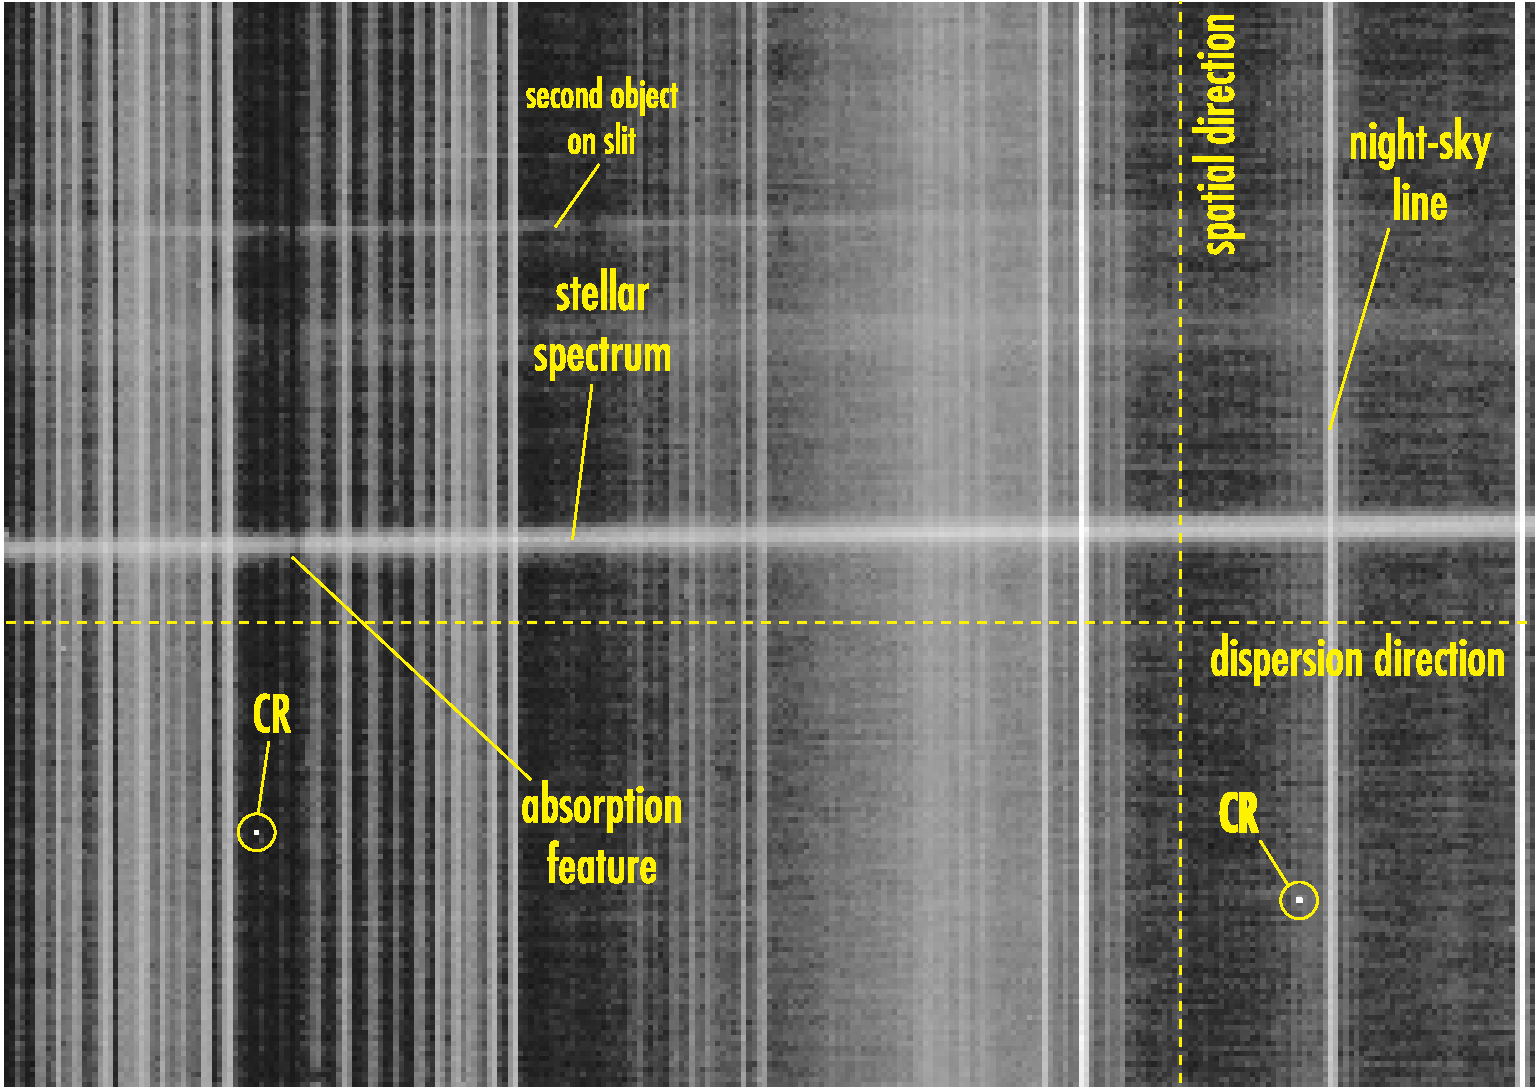
\includegraphics[height=105mm]{sc7_01}}
         {\leavevmode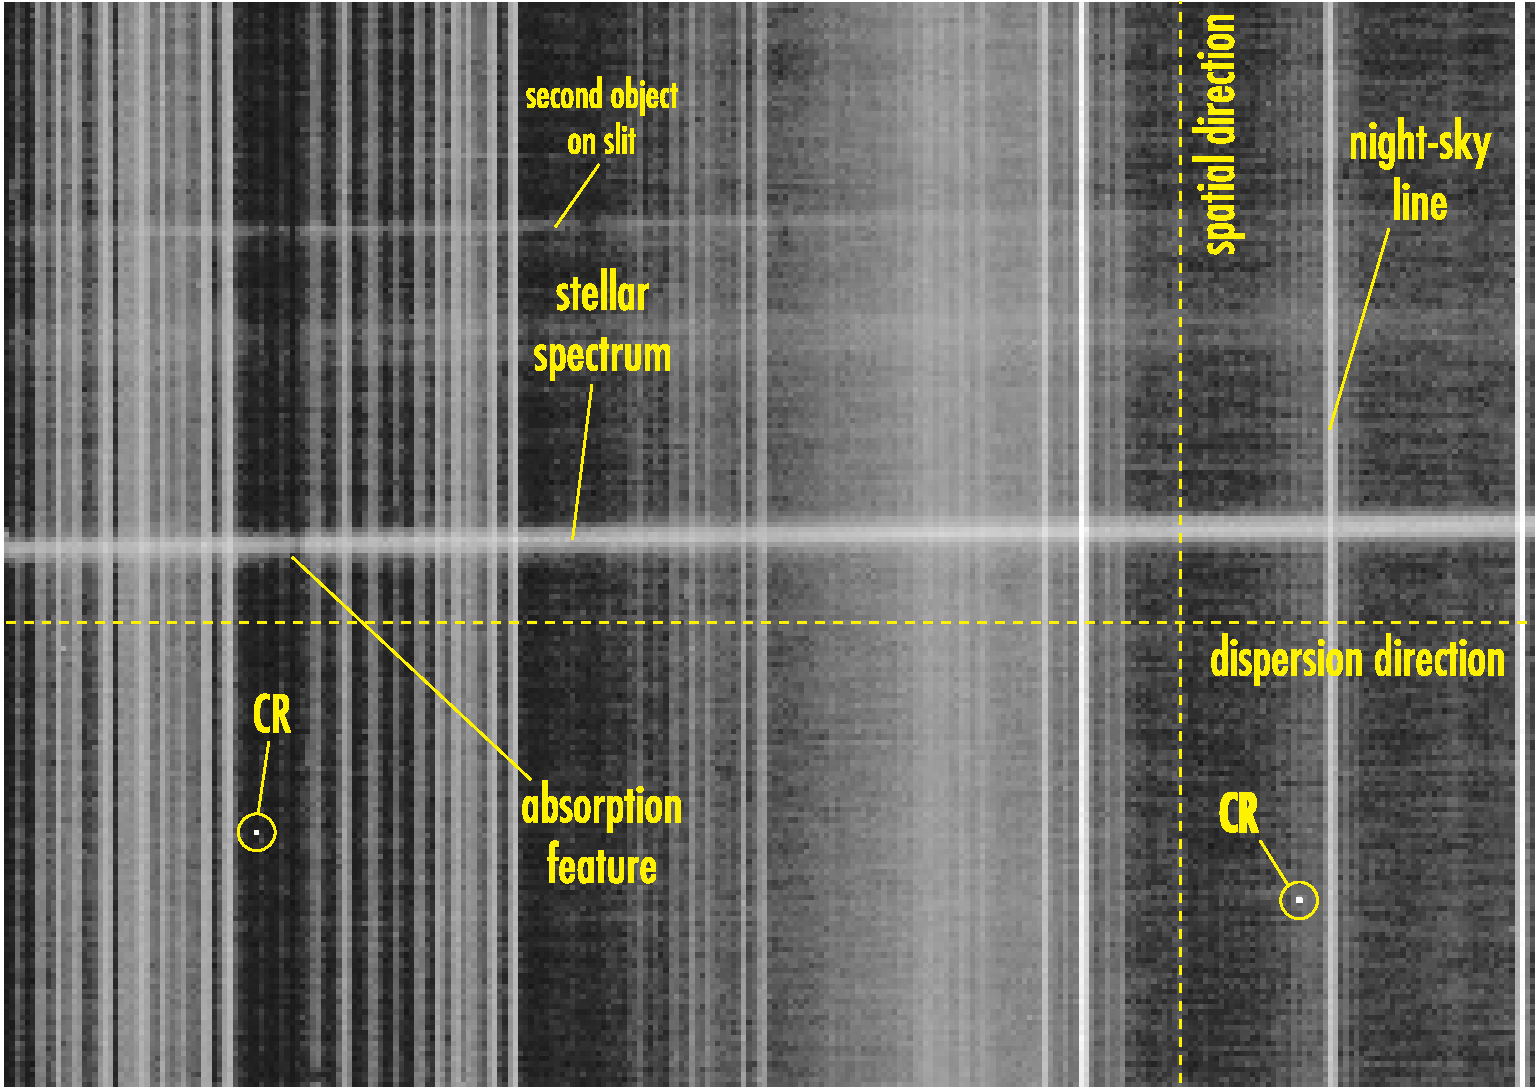
\includegraphics[height=136mm]{sc7_01}}

  \parbox{140mm}{
    \caption{Basic characteristics of a simple 1-D spectrum.}
    \label{fi_simple_spectrum}
  }
\end{center}
\end{figure}

If we divide up the light collected from an astronomical object by
wavelength the result is a spectrum.  What use is this?  We can derive
a great deal of information about the object we are looking at: chemical
composition, velocities, temperatures, and densities.

\scspec{Figure~\ref{fi_simple_spectrum}}{The figure above}
shows some of the features of a typical spectrum.
These data were recorded in the manner most commonly used: with a
\htmlref{CCD}{gl_ccd}.
You can see some \htmlref{cosmic-ray features}{gl_cosmic_ray}
(bright spots caused by cosmic rays hitting the detector),
as indicated by the label `CR', and
there are some night-sky lines (bright features in the spectrum of
the light coming from the sky) running vertically across the spectrum.


\begin{figure}
\begin{center}
  \scspec{\leavevmode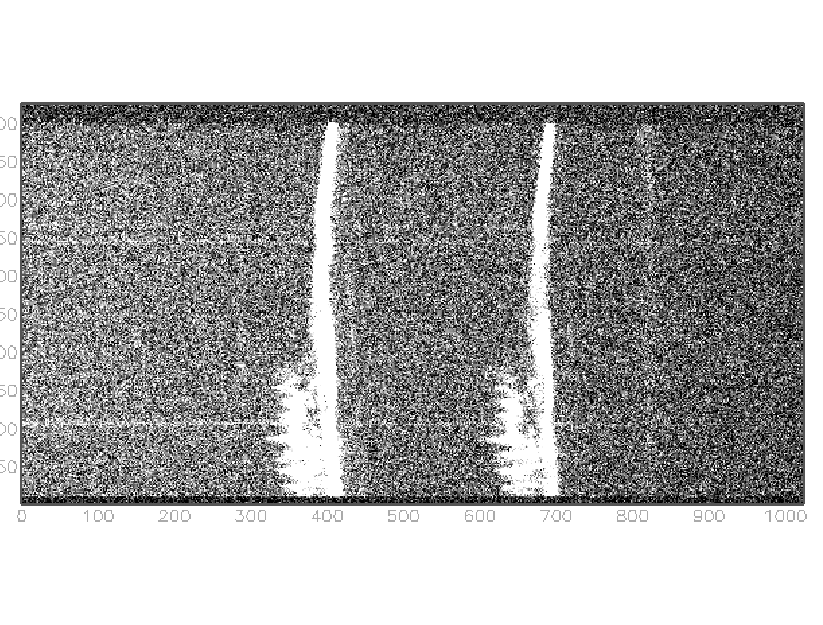
\includegraphics[height=105mm]{sc7_01b}}
         {\leavevmode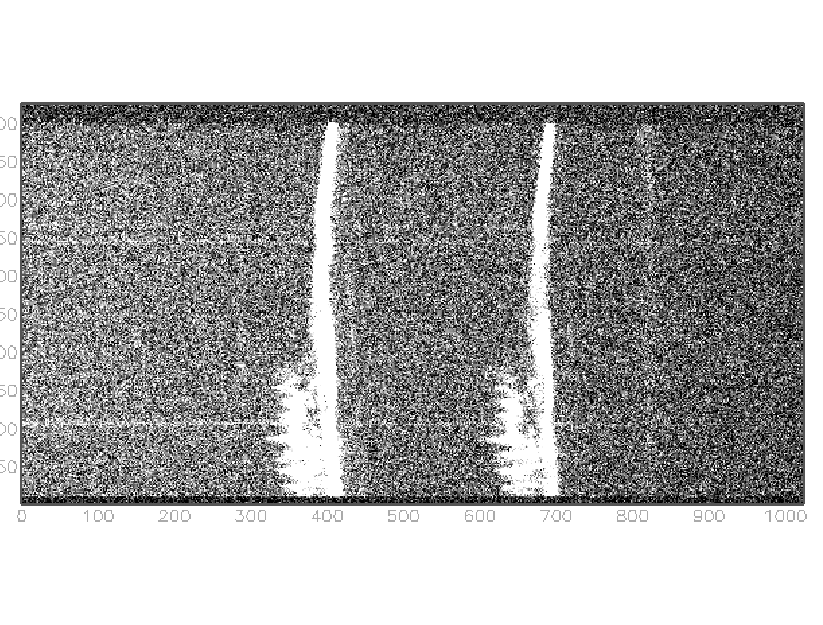
\includegraphics[height=136mm]{sc7_01b}}

  \parbox{140mm}{
    \caption{A longslit 2-D spectrum produces a number of spectra for
             positions along the slit length.}
    \label{fi_twod_spectrum}
  }
\end{center}
\end{figure}

Longslit spectroscopy produces CCD image frames which have essentially
the same features as are present in 1-D spectra (see
\scspec{Figure~\ref{fi_twod_spectrum}}{The figure above}. The
difference arises when the slit is placed over an extended object and
then an individual spectrum for each pixel row along the slit length
is obtained.

For consistency, all spectra discussed in this document are arranged
as in the above figures; the dispersion direction is oriented roughly
parallel to the X-axis, the spatial direction parallel to the Y-axis.




%%%%%%%%%%%%%%%%%%%%%%%%%%%%%%%%%%%%%%%%%%%%%%%%%%%%%%%%%%%%%%%%%%%%%%%%%%%
\section{\mlabel{preparing_for_observing}Preparing for Observation}
\markboth{Preparing for Observation}{\stardocname}

In this section some notes on what to be aware of prior to an observing
run are given.
In outline: to successfully extract and calibrate spectra
a complete set of reference frames should be obtained at the telescope;
it's always easier to take more calibrations at the telescope than to
cope with poor data at the terminal.

You might want to refer to the more extensive discussion of
\htmlref{CCD}{gl_ccd} data calibration in UGCRI\cite{ugcri},
the section entitled, `How Many and What Calibration Frames
Do You Need?'


\subsection{What CCD Data Do You Need?}

This is what you need to attempt `textbook' data preparation:

\begin{description}

\item [{\bf Bias frames}]
      Zero-second exposures taken with no signal light entering the
      instrument, but with any pre-flash used for the object exposures.

\item [{\bf Dark frames}]
      Long exposures taken with the shutter closed.  Typically, the
      exposure time used is similar to that selected for the object
      frames.

\item [{\bf Flat-field frames}]
      Exposures taken with a suitable \htmlref{continuum}{gl_continuum}
      lamp (usually Tungsten) as light source.

\item [{\bf Arc frames}]
      Exposures taken with an \htmlref{arc lamp}{gl_arc}
      (usually Thorium-Argon) as
      light source, to be used for \htmlref{wavelength
      reference}{gl_wavelength}.

\item [{\bf Object frames}]
      Exposures taken with a target object or reference object as the
      `light source'.

\end{description}

The arc and object frames will be processed by the data reduction software.
The bias, dark, and flat-field frames are used in the preparation of the
\htmlref{CCD}{gl_ccd} data.

Whether you actually need all these data frames, and how many of each
you need is to a large extent determined by what you hope to achieve.
In general, you will need a set of calibration frames for {\em each
night} of observing.


\subsection{Detector Pre-processing}

In order to remove detector-related effects a complete set of
\htmlref{bias}{gl_bias_frame}, \htmlref{dark}{gl_dark_frame},
and
\htmlref{flat-field}{gl_flat_field} frames should be obtained.
It is important to {\em
\htmlref{bracket}{gl_bracketing}} the science data exposures with
sets of \htmlref{CCD}{gl_ccd}
reference frames.  A post-observation review of these will reveal
any image shifts.  Having bracket frames allows the data to be
processed even in the event that some time-dependent variation
is found (as long as it is a small, slowly varying effect).

See \scspec{\S\ref{image_preparation}}
{\htmlref{{\sl Image Preparation}}{image_preparation}}
for outline details of CCD data preparation.

In some cases it may be possible to not use any
\htmlref{bias frames}{gl_bias_frame}.  Instead,
a median value for the bias level is obtained by inspecting the
\htmlref{overscan region}{gl_overscan} in some or all of the
object/arc frames.
You can use fewer bias frames when you have a high
signal-to-detector-noise ratio.

For exposure times limited by \htmlref{cosmic-ray event}{gl_cosmic_ray}
counts, the \htmlref{dark current}{gl_dark_current} in most CCD cameras
is not a significant factor.
The simplest way to decide whether to take dark frames is to take one
of exposure time similar to that you are using for object frames, and
check the signal level.


\subsection{\mlabel{flat_intro}Flat Fields}

You may not need to \htmlref{flat field}{gl_flat_field};
flats taken with modern \htmlref{CCDs}{gl_ccd} can be
uniform in response to only a few percent.
Flat fields are only needed if the signal-to-noise ratio
you require is high.
The precise figures will depend upon several factors,
and should be estimated for each observation.

You should try to match the configuration of telescope and instrument
in the flat-field and object exposures as closely as possible.
If there might be an image shift between flat fields taken before
observing and the science data, the best procedure is to take flats
\htmlref{bracketing}{gl_bracket} each science exposure in the same
way as you would take arcs.  Consult the instrument manual for your
\htmlref{spectrograph}{gl_spectrograph} to decide which strategy
to use.

See \scspec{\S\ref{flat_fielding}}
{\htmlref{Flat Fielding}{flat_fielding}} for details of
the purpose and use of flat-field frames.


\subsection{1-D Spectrum Tracing or 2-D Frame De-rotation}

If the CCD is not perfectly aligned with the dispersion axis of the
spectrometer then the data will be recorded at an angle to the grid of
dectector pixels. This can be corrected by tracing the spectrum (for
1-D data) or de-rotating the frame (for 2-D data).

It may be worth having {\em several} possible frames for
1-D spectrum tracing\scspec{---}{ - }in case some of them are badly
contaminated by cosmic rays and so difficult to use.

See \scspec{\S\ref{tracing}}{\htmlref{Tracing}{tracing}}
for more details on 1-D spectrum tracing.


\subsection{Wavelength Calibration}

As with the \htmlref{CCD}{gl_ccd} characterisation frames, two
wavelength-scale reference (\htmlref{arc}{gl_arc}) frames should be
taken \htmlref{bracketing}{gl_bracketing} the science exposures
{\em if} \htmlref{wavelength scales}{gl_wavelength} are required
({\it{e.g.}} for radial-velocity measurements)\@.
Normally you should find no significant difference between the two
extracted arc spectra; however, if you only take one arc exposure and
some shift does occur you won't be able to correct for it.
Using both arc spectra, a time-weighted mean wavelength scale can be
produced and applied to the science data.

See \scspec{\S\ref{wavelength_calibration}}
{\htmlref{Wavelength Calibration}{wavelength_calibration}}
for more details.

\subsection{Flux Calibration}

To get the best results when flux-calibrated spectra are wanted, select
reference stars as close as possible on the sky to your target objects.
You want the conditions of the target and reference
exposures\scspec{---}{ - }both instrument configuration and
\htmlref{air mass}{airmass}
through which the observations are made\scspec{---}{ - }to be as
similar as possible.

Refer to \scspec{\S\ref{finishing}}{\htmlref{{\sl{Finishing}}}{finishing}}
for more information on flux calibration.


%%%%%%%%%%%%%%%%%%%%%%%%%%%%%%%%%%%%%%%%%%%%%%%%%%%%%%%%%%%%%%%%%%%%%%%%%%%
\section{\mlabel{basic_reduction_steps}Basic Steps in 1-D Data Reduction}
\markboth{Basic 1-D Reduction Steps}{\stardocname}

In this section each of the basic steps in the spectral data reduction
procedure are described.
Examples of practical techniques using these ideas are to be found
in \scspec{\S\ref{simple_worked_example}}
{\htmlref{A 1-D Worked Example}{simple_worked_example}}.


\subsection{\mlabel{image_preparation}Image Preparation}

Most spectral data will be obtained using a \htmlref{CCD}{gl_ccd}.
Careful preparation of CCD data prior to attempting the extraction of
science data is essential.
In this Cookbook the procedure is outlined (very!) briefly.
Those points important to spectral data reduction are included.

The basic steps are:

\begin{description}

\item [{\bf Generate master \htmlref{bias frame}{gl_bias_frame}}]
      Typically done by finding the median of several bias frames.

\item [{\bf Subtract master bias frame}]
      The median bias frame is subtracted from each arc frame,
      object frame, and flat-field frame.

\item [{\bf Generate master \htmlref{flat-field frame(s)}{gl_flat_field}}]
      Again, done by finding the median of several (flat-field) frames.

\item [{\bf Crop images}]
      Regions\scspec{---}{ - }such as the overscan\scspec{---}{ - }are
      not used in the extraction process and should be removed (the same
      as cropping a photograph) as they may confuse the algorithms in
      the data reduction software.
      Often CCD images will have `rough' edges, {\em i.e.} non-useable
      data, which should also be cropped.

\end{description}

Depending on your source data and choice of reduction software you may
need to:

\begin{description}

\item [{\bf Rotate and orient the image}]
      All the major packages constrain the orientation of the spectra
      in some way.
      The images may have to be adjusted to meet these constraints.
      In general, if the spectra in your data run roughly
      horizontally (parallel to the X-axis) and the wavelength increases
      from left to right you will be fine.
      In other situations, you may need to use some utilities to
      re-orient the data.
      This may involve rotating and perhaps reflecting the images.

\end{description}

You may have data which contain \htmlref{dead columns}{gl_dead_column} or
few-pixel \htmlref{hot-spots}{gl_hotspot}.
Handling of these is discussed in the documentation for the CCD data
preparation packages.

Once a set of arc and object images have been prepared, the data
reduction process can begin.


\subsubsection{Software for CCD Data Preparation}

There are several packages for preparing \htmlref{CCD}{gl_ccd} data.
All of them offer similar functionality.
You'll find that it's easiest to use the package which complements
the spectral reduction software you choose.
There are two popular Starlink packages which you might use:
\xref{{\sc ccdpack}}{sun139}{} and \xref{{\sc figaro}}{sun86}{}\@.
{\sc ccdpack} includes some tools for conveniently managing the preparation
of many frames and supports the propagation of errors.
It also has a GUI-based interface for setting up automated reductions.
CCDPACK also has better facilities for combination of images, offering
several estimators.
In IRAF the {\tt noao.imred.ccdred} package should be used for CCD
data preparation.


\subsection{\mlabel{finding_spectrum}Finding the Spectrum in the Image}

\begin{figure}
\begin{center}
  \scspec{\leavevmode
\includegraphics[height=105mm]{sc7_02}}
          {\leavevmode
\includegraphics[height=136mm]{sc7_02}}

  \parbox{140mm}{
    \caption{A cross-section through a simple spectrum.}
    \label{fi_spectrum_locate}
  }
\end{center}
\end{figure}

A spectrum running parallel to the X-axis of an image can
be located by taking a cross-section (sometimes called a {\em slice} or {\em
cut}) parallel to the Y-axis.  For a simple spectrum, a plot of such a
section will appear as in \scspec{Figure~\ref{fi_spectrum_locate}}{the figure
above}.
If the spectrum is
faint, or has strong absorption features, it may be better to take the
median of several columns and use this to investigate the spatial profile
of the spectrum.  This will avoid the case where a single-column section
passes through the spectrum and there is no signal as, for example, in a
strong absorption feature.


\subsection{\mlabel{selecting_channels}Choosing the Object and Background
            Channels}

Once we know which row of the image the spectrum is centered on, we can
proceed to investigate the spatial profile by re-plotting the
cross-section
`zoomed in', centred on that row.
\scspec{Figure~\ref{fi_channel_select}}{The first figure below}
(left) shows such a plot.
The object spectrum has a width at the base of about 18 pixels.
We want to sum the signal from 9 pixels to the left of profile
centre, to 8 pixels to the right of profile centre to give the
gross spectrum for this object.
On either side of the spectrum are flatter areas which we have
chosen as background channels.
We could take the median value of these areas to give a measure
of the background.
The background level in the object channel can then be estimated
by taking the median of these values.
In \scspec{Figure~\ref{fi_channel_select}}{the first figure below},
the left-hand background channel runs from 10- to 16-pixels to the
left of the profile, and the right-hand channel from 9- to 14-pixels
to the right of the profile.

\begin{figure}
\begin{center}
  \scspec{\leavevmode\includegraphics[height=55mm]{sc7_03}}
         {\leavevmode\includegraphics[height=66mm]{sc7_03}}

  \parbox{140mm}{
    \caption{Selecting object and background channels (left), and a
             similar case, with the right-hand background channel
	     adjusted to avoid a feature on the slit (right).}
    \label{fi_channel_select}
  }
\end{center}
\end{figure}

\scspec{Figure~\ref{fi_channel_select}}{The figure above} (right)
shows a more awkward case, the background is infected,
possibly by a \htmlref{cosmic-ray hit}{gl_cosmic_ray},
or more likely, by a second, faint object on the slit.
In this case the right-hand background channel has been made
smaller to avoid the feature.
Use as many `clean' background pixels as available\scspec{---}{ - }as
long as this does not degrade resolution in the dispersion direction
(see \scspec{\S\ref{extraction}}
{\htmlref{{\sl{Extracting the Spectrum}}}{extraction}}).
A larger number of pixels gives both a better background
estimate, and better rejection of cosmic rays.
We might use a linear fit to the backgrounds to allow for the fact
that the channels are asymmetrical.


\subsection{\mlabel{tracing}Tracing the Spectrum}

In practice, the spectra produced by an instrument are not aligned
precisely parallel to the pixels in the detector used to record them.
There are many reasons for this, not least that the effect of
atmospheric refraction at the blue and red ends of the spectrum is
different.
As the position of the centre of the spectrum is subject to shifts in the
spatial direction, we need to find the centre of the spatial profile of
the spectrum at points along the dispersion direction, and fit
a curve to these points.
This process is known as {\em tracing} the spectrum.
\scspec{Figure~\ref{fi_order_trace}}{The figure below} shows the
curve fitted to a trace overlaid on the image of the spectrum.

\begin{figure}
\begin{center}
  \scspec{\leavevmode\includegraphics[height=105mm]{sc7_05}}
         {\leavevmode\includegraphics[height=136mm]{sc7_05}}

  \parbox{140mm}{
    \caption{Trace of a spectrum overlaid on the image.}
    \label{fi_order_trace}
  }
\end{center}
\end{figure}

When summing the signal from each sample in the dispersion direction, the
positions of the object and background channels are re-centered relative to
the trace.  This ensures that the `software slit' used for the extraction
correctly samples the spectrum.

For a bright spectrum with a \htmlref{continuum}{gl_continuum}, tracing is
done easily; however, if the spectrum has strong absorption features or is
very faint, it can be difficult to find the trace centre along the whole
length of the spectrum.
There is no perfect way to overcome this problem.
The strategy you adopt in these cases will depend upon which frames
you have available; it may be adequate to use a flat-field with the
\htmlref{dekker}{gl_dekker}
stopped down; it may be adequate to use a bright reference star image.
As long as you have one frame which you can trace you can use this
as a \htmlref{{\em template}}{gl_template_order} for the extraction.
The template trace may have to be shifted to register with the science frames.
You can determine if this is needed by over-plotting the trace on
the science frame and inspecting the fit.
In the worst case of no frame proving suitable for tracing, the trace
path may be defined manually; try to avoid this if at all possible.


\subsection{\mlabel{flat_fielding}Flat Fielding}

A \htmlref{flat-field}{gl_flat_field} frame is needed to correct for the
pixel-to-pixel sensitivity variations in the detector (and the small-scale
variations in the throughput of the instrument optics).
When imaging, an evenly illuminated scene is used as the flat field.
For spectroscopy we would want to use a light source
which is `white', {\it{i.e.}}, the same brightness at all wavelengths.
In practice this is not possible and the lamp used for the flat
field has some wavelength-dependent variation in brightness.  (The effect
becomes greater as dispersion increases.)  To remove the response
of the lamp, a low-order curve is fitted to the
response\scspec{---}{ - }assuming the spectrum runs with dispersion parallel
to the X-axis, we collapse the flat-field frame by summing columns, producing
a `spectrum' for the lamp, then fit a curve to this spectrum.
\scspec{Figure~\ref{fi_flat_field}}{The figure below}
shows how one of these `spectra' might appear.
The spectrum has a simple, continuous shape with small-scale noise
superimposed.
Having fitted a curve, we divide the flat-field by it so as to leave
the small-scale sensitivity variations only.

\begin{figure}
\begin{center}
  \scspec{\leavevmode\includegraphics[height=55mm]{sc7_06}}
         {\leavevmode\includegraphics[height=66mm]{sc7_06}}

  \parbox{140mm}{
    \caption{A section through a typical flat field for spectroscopy
             (left) and the same flat field after the large-scale
	     curve has been divided out (right).  Produced using
	     \xref{{\sc echomop}}{sun152}{}.}
    \label{fi_flat_field}
  }
\end{center}
\end{figure}


\subsection{\mlabel{extraction}Extracting the Spectrum}

In the previous steps nothing has been done to the data;
instead, models of the data have been produced.  We have:

\begin{itemize}

\item a model of the path of the spectrum in the image,

\item a model of the object and background channels.

\end{itemize}

At this point we are ready to extract the spectrum.
The procedure can be very simple, at each sample point along the
dispersion direction we sum the signal from all the pixels selected
as object; we then subtract a value based upon the pixels in the
background channels.
The same extraction is applied to both the target and reference star
images (if any), as well as to the arc images.

The procedure outlined above is known as a `simple' or `linear' extraction.
In many cases such an extraction is adequate; however,
this method does not make the most of the data available.
A profile curve can be fitted to the spectrum {\em in the spatial direction}.
At the centre of the profile the signal is greatest;
on the outside, the signal falls off to the background level.
If we sum these pixels in an unweighted manner we are ignoring the
fact that the central pixels have a better signal-to-noise ratio as
compared to those at the outside.
To overcome this problem we use the so-called `optimal' extraction scheme.

Optimal extraction is suitable for \htmlref{CCD}{gl_ccd} data
when we know the \htmlref{readout noise}{gl_readout_noise} and
\htmlref{gain}{gl_gain} of the CCD camera.
The CCD readout noise is needed to calculate pixel weights.
The gain is used to convert the data in the input images, which are
in the `arbitrary' units from the camera \htmlref{ADC}{gl_adc}, to
units of recorded photons.
Once we have the data in these units, we can apply an error-based weighting
to the summation of data in each sample along the dispersion direction.

Optimal extraction assumes that a good model for the noise
sources in our data is available; this is a fair assumption as the noise
sources in a CCD camera system are well understood (well, at least at the
sort of level we are interested in anyway).
The main noise `sources' are: the camera electronics, the CCD output node,
and the shot noise of the electronic charge stored in a pixel (which
represents the light signal).
There are other sources\scspec{---}{ - }see Horne\cite{horne} and
Marsh\cite{marsh} for more details of the theory of optimal extraction.

\begin{figure}
\begin{center}
  \scspec{\leavevmode
\includegraphics[height=105mm]{sc7_07}}
         {\leavevmode
\includegraphics[height=136mm]{sc7_07}}

  \parbox{140mm}{
    \caption{An extracted spectrum.}
    \label{fi_extracted_spectrum}
  }
\end{center}
\end{figure}

In cases where the CCD parameters are not available, a profile-weighted
extraction might be used.  This weights the summation of the
object pixels based upon their relative brightnesses.
This should give a better signal-to-noise ratio than the simple
extraction.

Which extraction scheme you select will depend on the nature
of\scspec{---}{ - }and what you want from\scspec{---}{ - }your data.
For bright, high signal-to-noise data there is little to be gained
by going for an optimal extraction (little may be lost by doing one
though\ldots ).
Optimal-extraction algorithms require that the spatial profile of the
object is a smooth function of wavelength.
This means that optimal extraction is unlikely to be useful if spatial
resolution is required and/or the spatial profile of the object varies
rapidly with wavelength, as for objects with spatially-extended
emission-line regions.  For suitable data, optimal extraction also acts
as a \htmlref{cosmic-ray}{gl_cosmic_ray} filter: any pixel which deviates
strongly from the profile model is likely to be contaminated, and can be
rejected.


\subsection{\mlabel{wavelength_calibration}Wavelength Calibration}

Once the spectrum extraction is complete we have a two-dimensional
dataset: sample number and intensity.
(You may also have error data for each sample.)
Sample number is simply an index for each integration bin along the
spectrum ({\em{e.g.}}, the X-axis in \scspec{Figure~\ref{fi_echarc_plot}}
{the figure below}).
For some purposes this spectrum may be enough, but usually
the next step in the reduction process is to find the
relationship between wavelength and sample number.

The basic steps here are:

\begin{itemize}

\item Look at the arc (or comparison) spectrum and identify
      features of known wavelength.

\item Fit a low-order polynomial to the arc wavelength-sample relationship.

\item Paste the wavelength-sample relationship on to the object spectrum.

\end{itemize}

\begin{figure}
\begin{center}
  \scspec{\leavevmode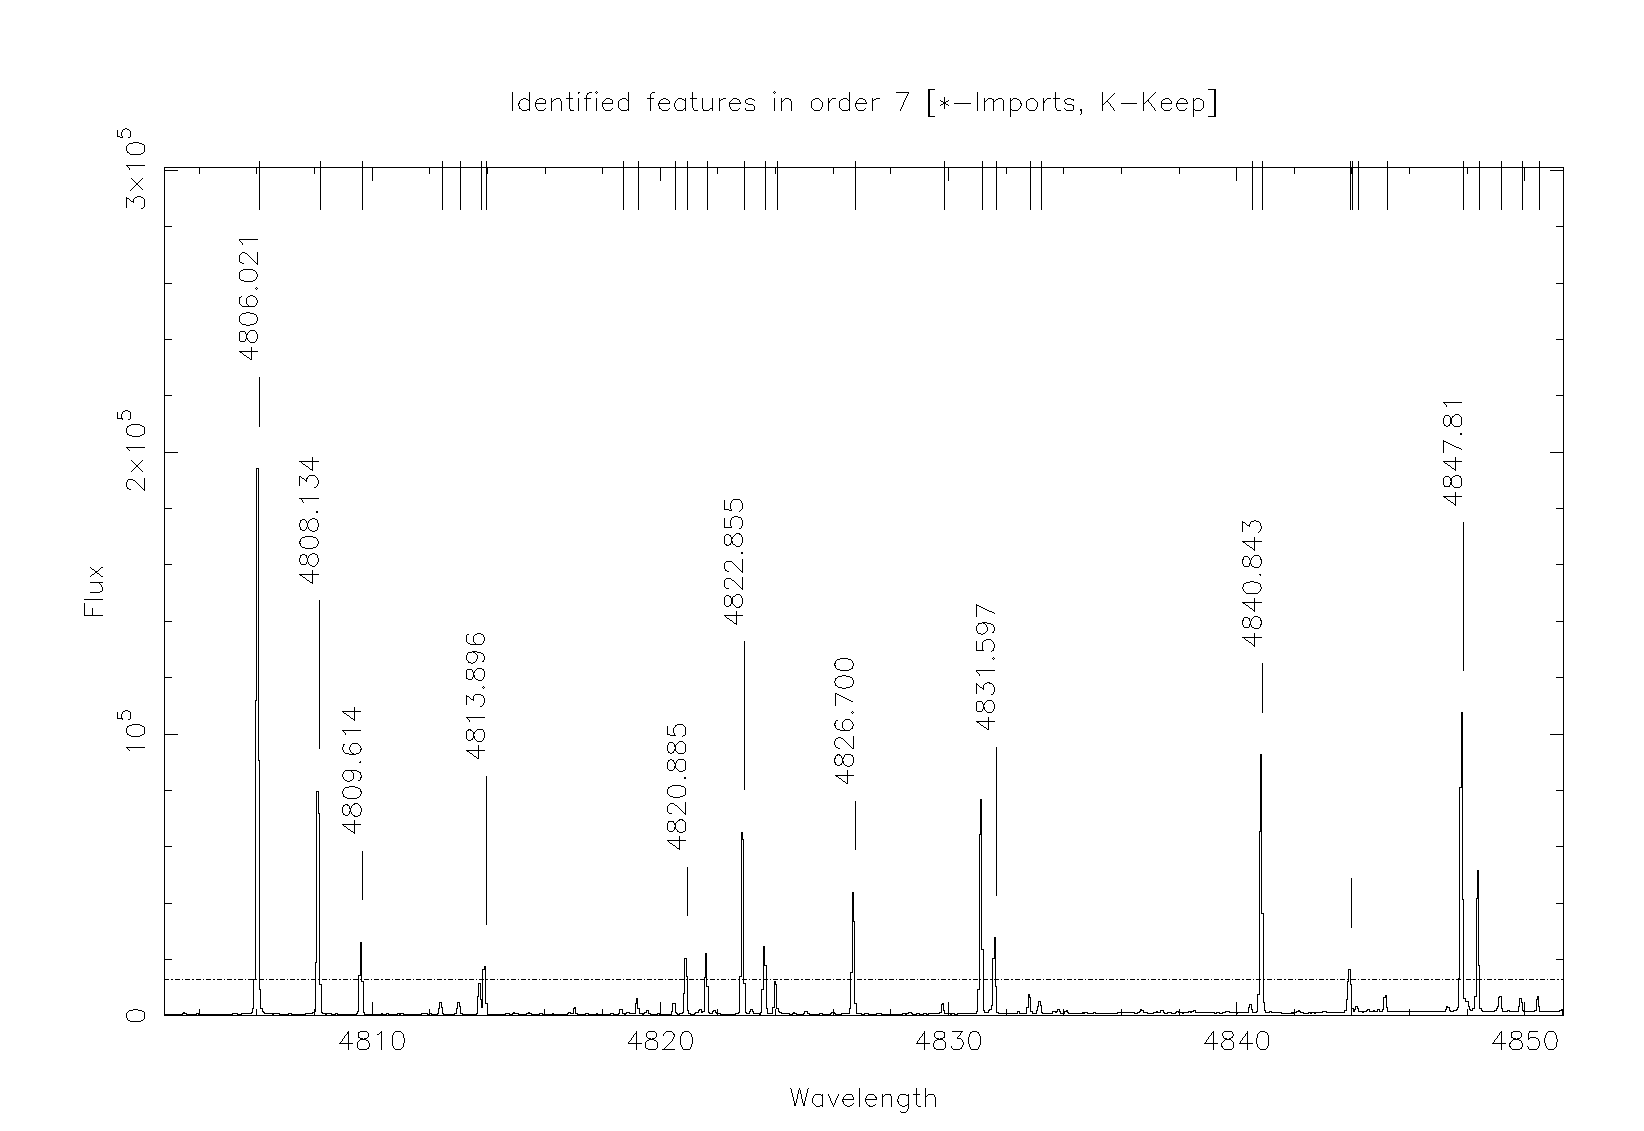
\includegraphics[height=105mm]{sc7_08}}
         {\leavevmode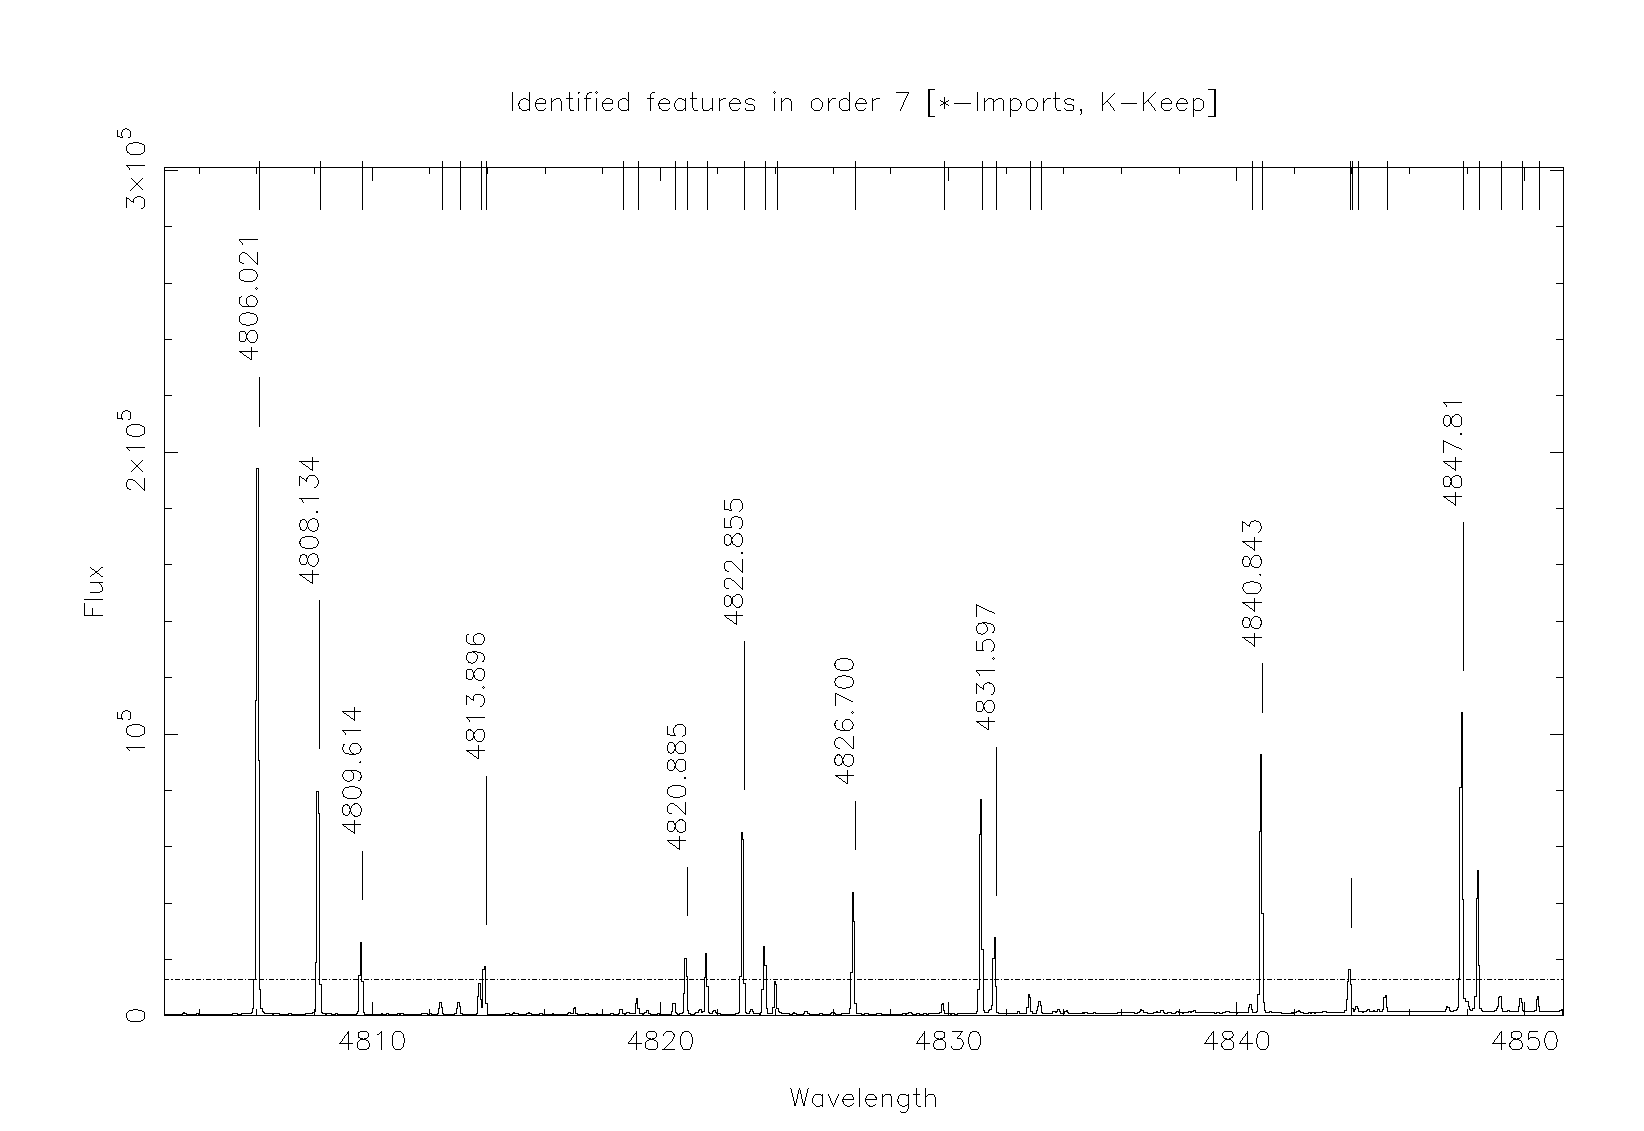
\includegraphics[height=136mm]{sc7_08}}

  \parbox{140mm}{
    \caption{Line Identification: a typical plot during interactive
             fitting with \xref{{\bf echmenu}}{sun152}{}.}
    \label{fi_echarc_plot}
  }
\end{center}
\end{figure}

\mlabel{atlases}
You should find that a list of spectral-feature wavelengths for
common arc reference lamps is available on-line (see
\scspec{\S\ref{example_wavelength_calibration}}{the \xref{worked
example}{example_wavelength_calibration}} for more details).
You may also be able to lay your hands on a hardcopy of a `mapped'
\htmlref{comparison spectrum}{gl_comparison} for your selected
\htmlref{arc lamp}{gl_arc},  perhaps obtained using
the same spectrograph as your data, this will consist of a plot
(or series of plots) of the spectrum annotated with rest wavelengths.
For example, Bessell \& Pettini\cite{echref} should be available
at most UK Starlink sites.
Some people prefer the \htmlref{ESO}{gl_eso} arc-line atlas\cite{eso_main}
in which the line wavelengths are easier to read.

Ideally an arc spectrum should contain at least three or four
identifiable spectral lines, preferably with one close to each
end of the spectrum, and one or more spread in the middle.
In some cases it may be useful to refer to the object and/or reference star
spectra to look for strong features of known, or approximately known,
wavelength.
These can be used to help you `home-in' on features in the arc spectrum.
When a fit is made to these features you will be advised of the
goodness-of-fit, usually in the form of a plot of line versus
deviation-from-fit or RMS deviation values for each line.
You will be able to adjust the fit and reject any lines which
seem to have been mis-identified, then re-fit the data.

\scspec{Figure~\ref{fi_echarc_plot}}{The figure above} shows a plot of a
single order during interactive line-identification using
\xref{{\bf echmenu}}{sun152}{}.

Once you have a complete wavelength-calibrated comparison spectrum you
can `copy' the wavelength scale onto your object spectra.
It may be useful to calibrate {\em two} arcs which
\htmlref{bracket}{gl_bracketing} the object exposure in time.
This will show any time-dependent variation in the wavelength scale.
If there is some change (and it is reasonably small) you can
take a time-weighted mean of the two bracketing wavelength scales and use
this for the object spectrum.


\subsection{\mlabel{finishing}Finishing Reduction}

Once you have a wavelength-calibrated spectrum you may (again)
be happy enough and not need to go any further.
It is more likely that you will want to do one of two things,
either flux calibrate, or normalise the spectrum.


\subsubsection{\mlabel{flux_calibration}Flux Calibration \&
               Extinction Correction}

If, as part of your observing programme, you take spectra of standard stars
then you will be able to attempt to flux calibrate your data.

The flux-calibration process is simple: you compare the extracted
standard-star spectrum to a published spectrum of the same star.  At each
`wavelength' (I use the term very loosely here\scspec{---}{ - }see below for a
proper explanation) you find the ratio of the observed to published spectrum.
The result is a conversion factor at each `wavelength'.
To flux calibrate your target objects you multiply the spectra by these
per-wavelength conversion factors.  The effect of this is to remove
instrumental-response wavelength-dependency.  At least that's the
idea\ldots\ in practice, you must be careful to understand how the
published standards are tabulated, and how this might relate to your data.

\paragraph{How Standards are Tabulated}

There are two ways in which the standard-star data are tabulated,
both are tables of fluxes versus wavelengths:
in one, each point has a corresponding pass-band width;
in the other, each point is a fit to a
\htmlref{continuum}{gl_continuum} curve.
In the first case, the published standard and your observed standard should
look the same once the flux in the appropriate pass bands has been
summed\scspec{---}{ - }even when absorption features are present in the
spectrum.  In the second case you must either fit a continuum to your
data or, if there are no absorption features present in the wavelength range
covered, you might just interpolate between the points in the published
standard.

\paragraph{\mlabel{airmass}Air mass \& Extinction}

The Earth's atmosphere absorbs and reddens light from astronomical sources.
The effect is dependent upon many factors: weather, observing site, time of
year, time of day (or night), and so on.
The process is known as {\sl atmospheric extinction.}
The depth of atmosphere through which an object is
observed is another factor determining the extinction.
This depth is known as {\sl air mass.}

When an object lies at the zenith the depth of atmosphere
through which it is observed is one air mass.
As the zenith angle of the object increases, so does the air mass.

The effect of extinction is wavelength-dependent and so a table of
correction factors is required.
Each observatory should have such a table available for its site.

You should observe your standard star through as similar an air mass
to the target as possible.  Unless the standard is very close to the
target, and both are at a fairly high altitude, you may still need to
compensate for differential extinction, rather than simply assuming the
atmosphere has the same effect on both observations.  It may be a good
strategy to observe your standards at a range of different altitudes
throughout a night, then fit a curve to these and interpolate to
calibrate the science observations.

If you are fortunate, the air mass for a particular observation will
automatically be present in the FITS headers of your
data\scspec{---}{ - }otherwise you will have to calculate it.


\subsubsection{\mlabel{normalisation}Normalisation}

\begin{figure}
\begin{center}
  \scspec{\leavevmode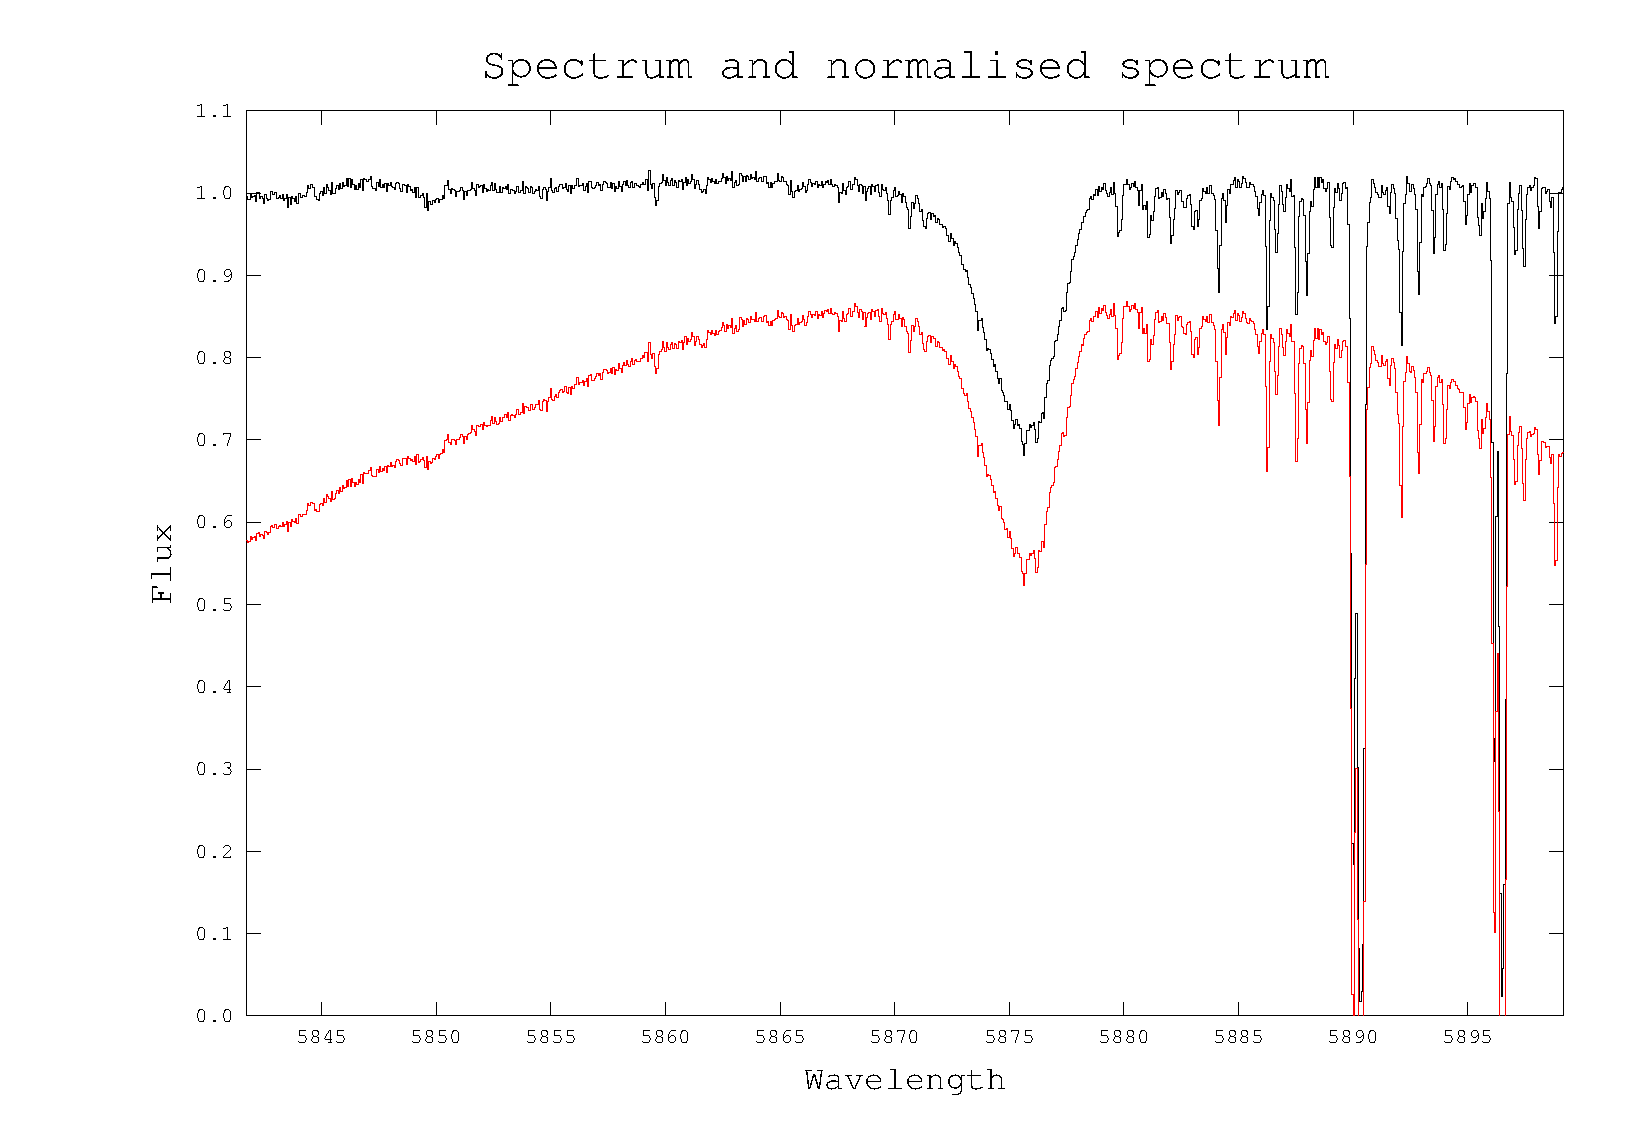
\includegraphics[height=105mm]{sc7_09}}
         {\leavevmode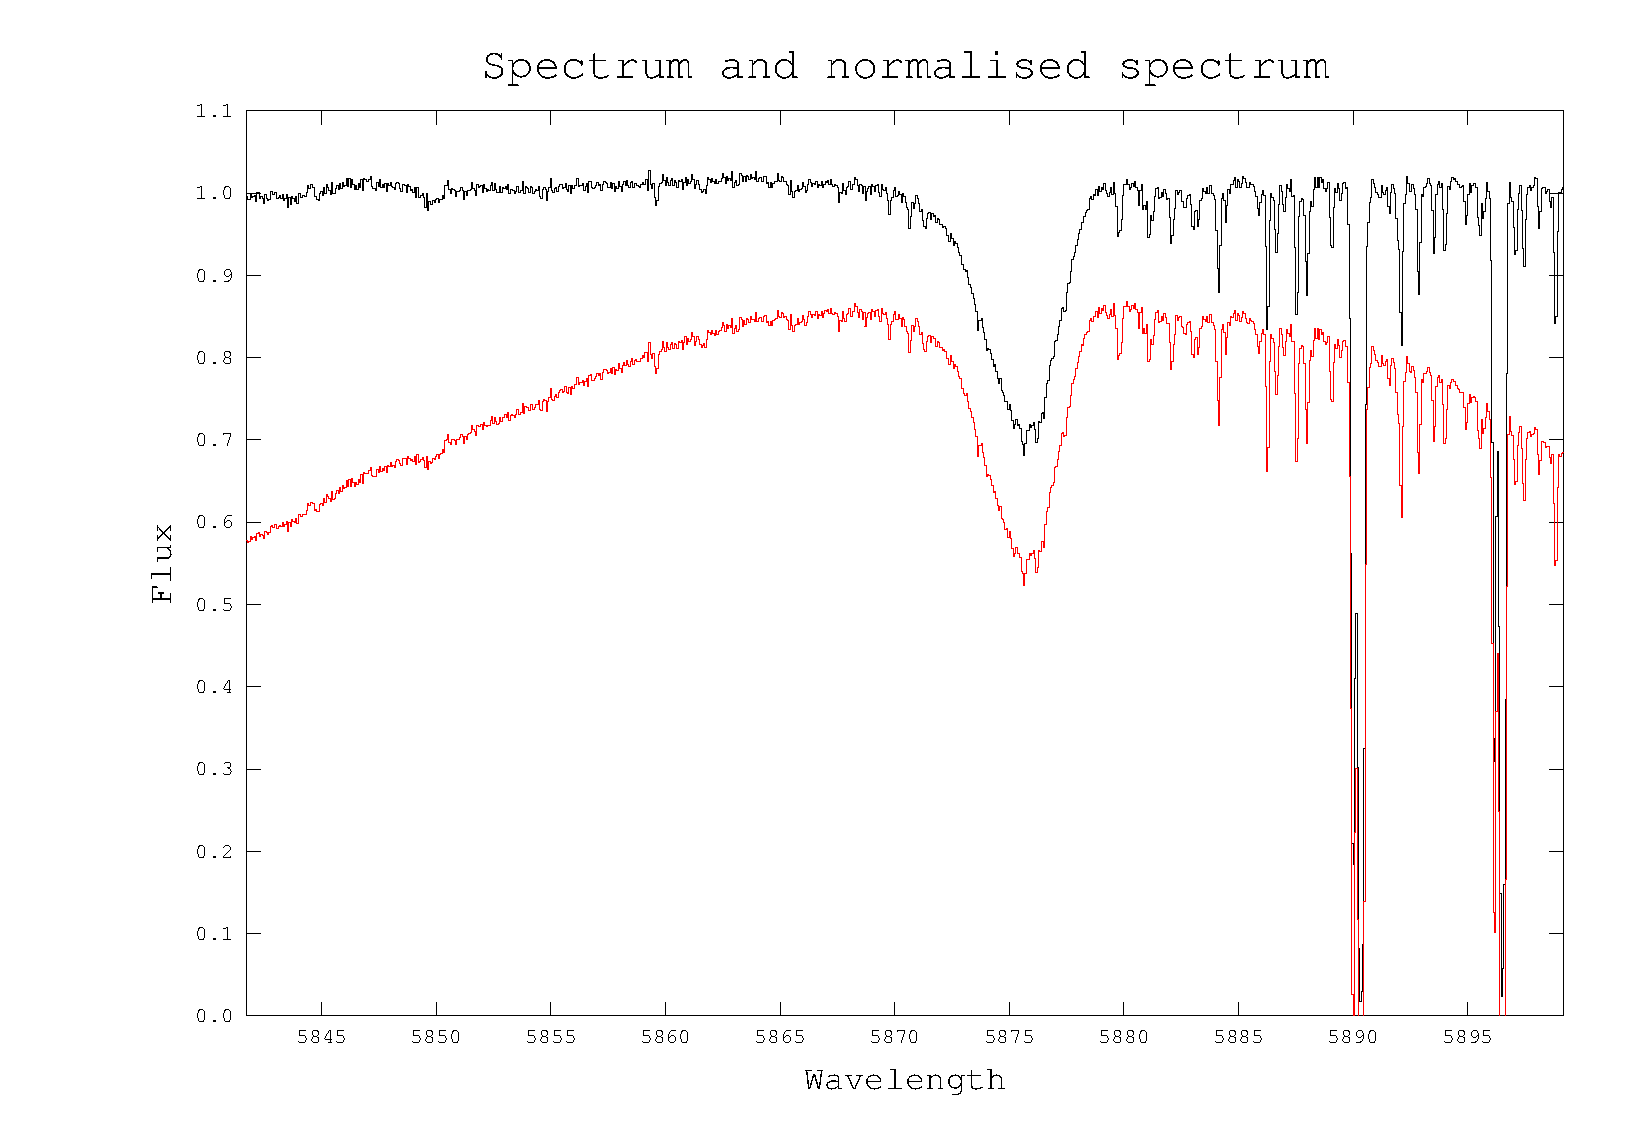
\includegraphics[height=136mm]{sc7_09}}

  \parbox{140mm}{
    \caption{Normalisation: the top spectrum is the normalised version
             of the lower spectrum.  Note that the flux values in the
	     uncorrected spectrum have been scaled and shifted for
	     this plot.}
    \label{fi_normalise}
  }
\end{center}
\end{figure}

If you are not flux calibrating your data then you will probably want to
remove the low-frequency instrument profile from the data.  This process
is known as normalisation or blaze correction.
\scspec{Figure~\ref{fi_normalise}}{The figure above} shows a plot of
a spectrum and the same spectrum after normalisation.
The continuum is more or less flat in the corrected spectrum.
Normalisation can be useful when you want to look at absorption line
profiles, model their shapes, or determine their widths.

There are several approaches to normalising the data.
One method is to fit a polynomial or other curve to the
spectrum and then divide it by the curve.
This often works; however, it may well be necessary to manually
select which parts of the spectrum to fit as strong spectral
features will lead to a poor fit to the continuum.
Another method is to `draw' points of the continuum on to a plot
of the spectrum and fit a curve to these points.
This is usually an entirely manual process.

Another method is to fit a curve to the extracted `spectrum' of a
flat field and use that for normalisation.
As for the object spectra, this method will only work if the flat-field
is devoid of strong spectral features (which it should be, otherwise it
isn't much use for flat-fielding).


%%%%%%%%%%%%%%%%%%%%%%%%%%%%%%%%%%%%%%%%%%%%%%%%%%%%%%%%%%%%%%%%%%%%%%%%%%%
\section{\mlabel{simple_worked_example}A Worked Example}
\markboth{Example Reduction}{\stardocname}

In this section, a simple run-through of the extraction process using
Starlink software is given.
\scspec{\S\ref{cookies}}{The \htmlref{cookies}{cookies} section}
gives answers to specific questions and solutions to common problems.

Before you start the extraction you will have to do the
detector-specific preparation of your data (most likely to remove
CCD-related effects).
If you have not done this, refer to \scspec{\S\ref{image_preparation}}
{\htmlref{Image Preparation}{image_preparation}} for an outline of the
procedure, and \scspec{\S\ref{other_sources}}
{\htmlref{Other Sources of Information}{other_sources}} for pointers
to documentation of the process.


\subsection{Setting Up}

The first thing you need to do (if you've managed to prepare your CCD
data you will most likely know this already, but\ldots ) is to run the
Starlink setup.
Normally Starlink software is installed in the \verb+/star+ directory
and the commands you must execute are:

{
\scspec{\small}{ }
\begin{verbatim}
   % source /star/etc/cshrc
   % source /star/etc/login
\end{verbatim}
}

If your Starlink software is installed somewhere other than
\verb+/star+---one place to look is \verb+STARLINK_DIR+---then
modify the commands appropriately.  Most people include these lines in
their shell login file (\verb+.login+ in your home directory).

Once you have done the Starlink `login' you can initialise for any of the
major packages simply by typing their names.
For example, we are going to use
\xref{{\sc kappa}}{sun95}{}\cite{kappa} and
\xref{{\sc echomop}}{sun152}{}\cite{echomop} and so get a display
something like:

{
\scspec{\small}{ }
\begin{verbatim}
   % kappa    # Only needed once per session.

      KAPPA commands are now available -- (Version 0.9-3)
      KAPPA uses NAG routines, by permission of NAG ltd.

      Type kaphelp for help on KAPPA commands
      Type "showme sun95" to browse the hypertext documentation

   % echomop  # Only needed once per session.
    ----------- Initialising for ECHOMOP ------------
                 Echelle data reduction
            Version 3.2-0  9th December 1996

             Type "echhelp echomop" for help
       or "echhelp news" for news on changes

    Type "echwww" to start Mosaic documentation browser.
    Type "echmenu" to start the monolith.
\end{verbatim}
}

We can now use {\sc kappa} commands and
\xref{{\bf echmenu}}{sun152}{ECHMENU},
the menu-driven front-end for {\sc echomop}.

At this point you might like to take a copy of the example data which comes
with this document when installed as part of the Starlink document set.
You will find the files in the directory

{
\scspec{\small}{ }
\begin{verbatim}
   /star/examples/sc7/
\end{verbatim}
}

Create an empty directory and enter it using {\bf cd}\@.
To copy the test data type the command

{
\scspec{\small}{ }
\begin{verbatim}
   % /star/examples/sc7/copydata
\end{verbatim}
}

You will then find you have these datafiles in your directory:

\begin{latexonly}
\begin{center}
\begin{tabular}{ll}
File & Description \\ \hline
{\tt object.sdf}  & Frame with the object spectrum\\
{\tt flat.sdf}    & Frame with a flat field\\
{\tt arc.sdf}     & Frame with a wavelength-reference arc\\
{\tt object1.sdf} & Frame with a rotated spectrum\\ \hline
\end{tabular}
\end{center}
\end{latexonly}
\begin{htmlonly}
\begin{verbatim}
File         Description
object.sdf   Frame with the object spectrum
flat.sdf     Frame with a flat field
arc.sdf      Frame with a wavelength-reference arc
object1.sdf  Frame with a rotated spectrum
\end{verbatim}
\end{htmlonly}

\subsection{\mlabel{inspecting_the_images}Inspecting the Images}

The first thing you need to do is ensure that the images are oriented
correctly.  To do this use \xref{{\sc kappa}}{sun95}{}
\xref{{\bf display}}{sun95}{DISPLAY} to look at the image:

{
\scspec{\small}{ }
\begin{verbatim}
   % idset xwindows
   % display object mode=pe accept
   % lutspec
\end{verbatim}
}

This will display the image \verb+object+ using a false-colour
look-up table.  You may have to use the
\xref{{\bf xdisplay}}{sun129}{}\cite{xdisplay} command to ensure
that the image is sent to the correct ({\it{i.e.}} your) screen.
{\bf display} has many
options, for the moment we just need to check the orientation of the image,
the \verb+accept+ keyword tells {\sc kappa} to use default values for the
parameters we have not given.
The example data are correctly oriented, with the spectrum dispersion
from left-to-right.

Try

{
\scspec{\small}{ }
\begin{verbatim}
   % display object1 clear mode=pe accept
\end{verbatim}
}

The \verb+clear+ parameter indicates that we want the previous display to
be erased before \verb+object1+ appears.
You'll see that this spectrum looks similar to the previous one, but it runs
from top-to-bottom of the image\scspec{---}{ - }it needs to be rotated.
To do this, use the {\sc kappa} command \xref{{\bf rotate}}{sun95}{ROTATE}.

{
\scspec{\small}{ }
\begin{verbatim}
   % rotate object1 object1r 90
\end{verbatim}
}

This rotates the data in \verb+object1+ clockwise by 90 degrees and places
the result in \verb+object1r+\@.  If you find that your real data need to be
rotated, you will have to apply the change to all the data files (including
arcs and flat fields).  Try this to inspect the rotated data:

{
\scspec{\small}{ }
\begin{verbatim}
   % display object1r clear accept
\end{verbatim}
}

Jumping ahead (quite a way) you may want to ensure that the now correctly
rotated data are arranged so that the spectrum is dispersed with wavelength
increasing from left-to-right.  Don't worry if you don't know how to do
this\scspec{---}{ - }it isn't strictly necessary; however, you may find it
easier to recognise the arc spectrum in an atlas if it is arranged with the
wavelength increasing left-to-right as this is the way the atlases are
printed.
You can always come back later and flip the images if you find the arcs hard
to recognise.
There's no single way to spot which way the spectra are dispersed.
You have to know a little about the spectra you are working with;
where the strong or large features are.  You might look at the arc as
well for some familiar pattern in the reference spectrum.

If you do find that you need to reverse the dispersion direction, you can use
{\sc kappa} \xref{{\bf flip}}{sun95}{FLIP} to do this:

{
\scspec{\small}{ }
\begin{verbatim}
   % flip object1r object1rf 1
\end{verbatim}
}

This tells {\sc kappa} to flip the first (X-) axis in the data and put
the resulting image in the dataset \verb+object1rf+\@.
You can see here the common practice of appending letters to the
dataset names to indicate what processing they have
undergone\scspec{---}{ - }`r' for rotate, `f' for flip.
This can be helpful if you have many images and are going to work
over several sessions.

We can now proceed to the first stage in the actual spectrum extraction.


\subsection{Locate the Spectrum}

The spectrum extraction is done using the \xref{{\sc echomop}}{sun152}{}
package.  At this stage, you will find it easiest to work through the
example extraction here, rather than trying to understand all the
facilities and parameters of {\sc echomop}.

The first stage is to start \xref{{\bf echmenu}}{sun152}{ECHMENU}:

{
\scspec{\small}{ }
\begin{verbatim}
   % echmenu ech_rdctn=rdf1 display=yes soft=xwindows tune_mxskypix=31
   This is ECHOMOP Version 3.2-0.
    ... setup messages ...
    Main menu options:
     0. HELP/HYPER (ASCII or hypertext help).
     1. Start a reduction.                 16. Check trace consistency.
     2. Trace orders.                      17. Post-trace Cosmic Ray locate.
    ... other options ...
    14. Save reduced data.                 29. System () commands.
    15. Plot order traces.                 30. Output balance-factor frame.
                                           31. EXIT (alias Q/E/QUIT/EXIT/99).
    Use -nn to edit/view option parameters.
    - Option number /'or Y for default=1'/ >
\end{verbatim}
}

Each reduction is described by a database file specified by the
\xref{{\tt ech\_rdctn}}{sun152}{par_ECH_RDCTN} parameter,
in this case we have chosen \verb+rdf1+, which the program creates.
The \verb+display+ parameter tells {\bf echmenu} to overlay trace
plots  on the image itself so we can see how well the trace is doing.
The \xref{{\tt soft}}{sun152}{par_SOFT} parameter points output
graphs to our existing \verb+xwindows+ screen.
Don't worry about \xref{{\tt tune\_mxskypix}}{sun152}{par_TUNE_MXSKYPIX}
for now, it is needed (and explained) later on.

{\bf echmenu} displays its complete menu\scspec{---}{ - }most of the options
are specialised and we don't need them at this stage.
{\bf echmenu} works through the extraction process in a series of numbered
steps (1, 2, 3, etc\ldots).  You can exit {\bf echmenu} between stages
and return later to pick up the reduction at the same point.
{\bf echmenu} tends to be quite verbose when displaying
messages\scspec{---}{ - }don't be put off by this, most of the information
is not useful at this stage and can simply be ignored.
For brevity, most of these messages are not included in future screen
display listings.

The prompt at the end of the above display is suggesting
\xref{Option~1 {\sl Start a reduction}}{sun152}{option1}
which seems like a good place to begin:

{
\scspec{\small}{ }
\begin{verbatim}
    - Option number /'or Y for default=1'/ > 1
   TRACIM - Frame for order tracing /''/ > object
    ... messages ...
   INPTIM - Frame to extract data from /''/ > object
    ... messages ...
   ARC - Name(s) of reference (arc) lamp image(s) /''/ > arc
    ... messages ...
    Current number of orders: 1.
    Options:
      A - Add an order.
      D - Delete an order.
      C - Clear (delete all orders).
      R - Re-plot.
      E - Exit.
      M - Full menu display.
\end{verbatim}
}

There are three prompts which appear: first,
\xref{{\tt{tracim}}}{sun152}{par_TRACIM} is asking which
image to use to trace the path of the spectrum\scspec{---}{ - }in this case
we are able to use the object itself;
\xref{{\tt{inptim}}}{sun152}{par_INPTIM} is asking for the name of
the file from which the spectrum will be extracted, again this is
\verb+object+; lastly,
\xref{{\tt{arc}}}{sun152}{par_ARC} is the name of the wavelength-reference
image, which is called \verb+arc+ in the example data.

\begin{figure}
\begin{center}
  \scspec{\leavevmode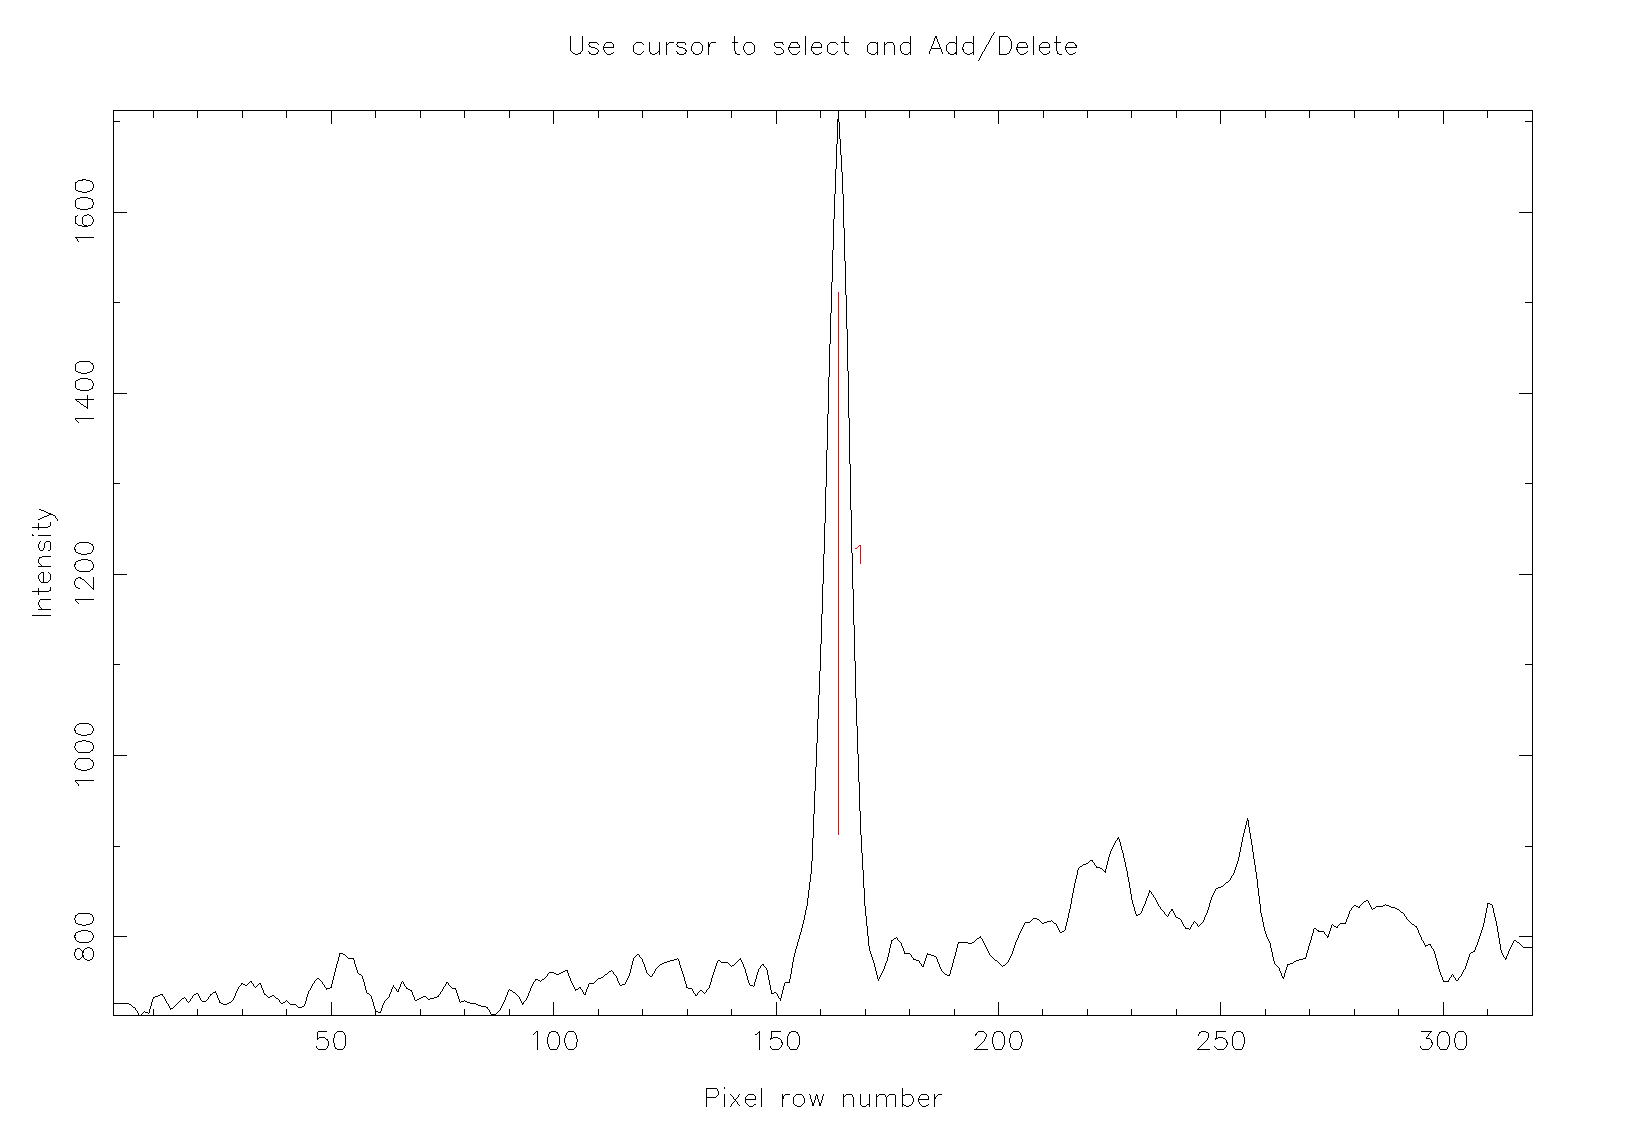
\includegraphics[height=100mm]{sc7_10}}
         {\leavevmode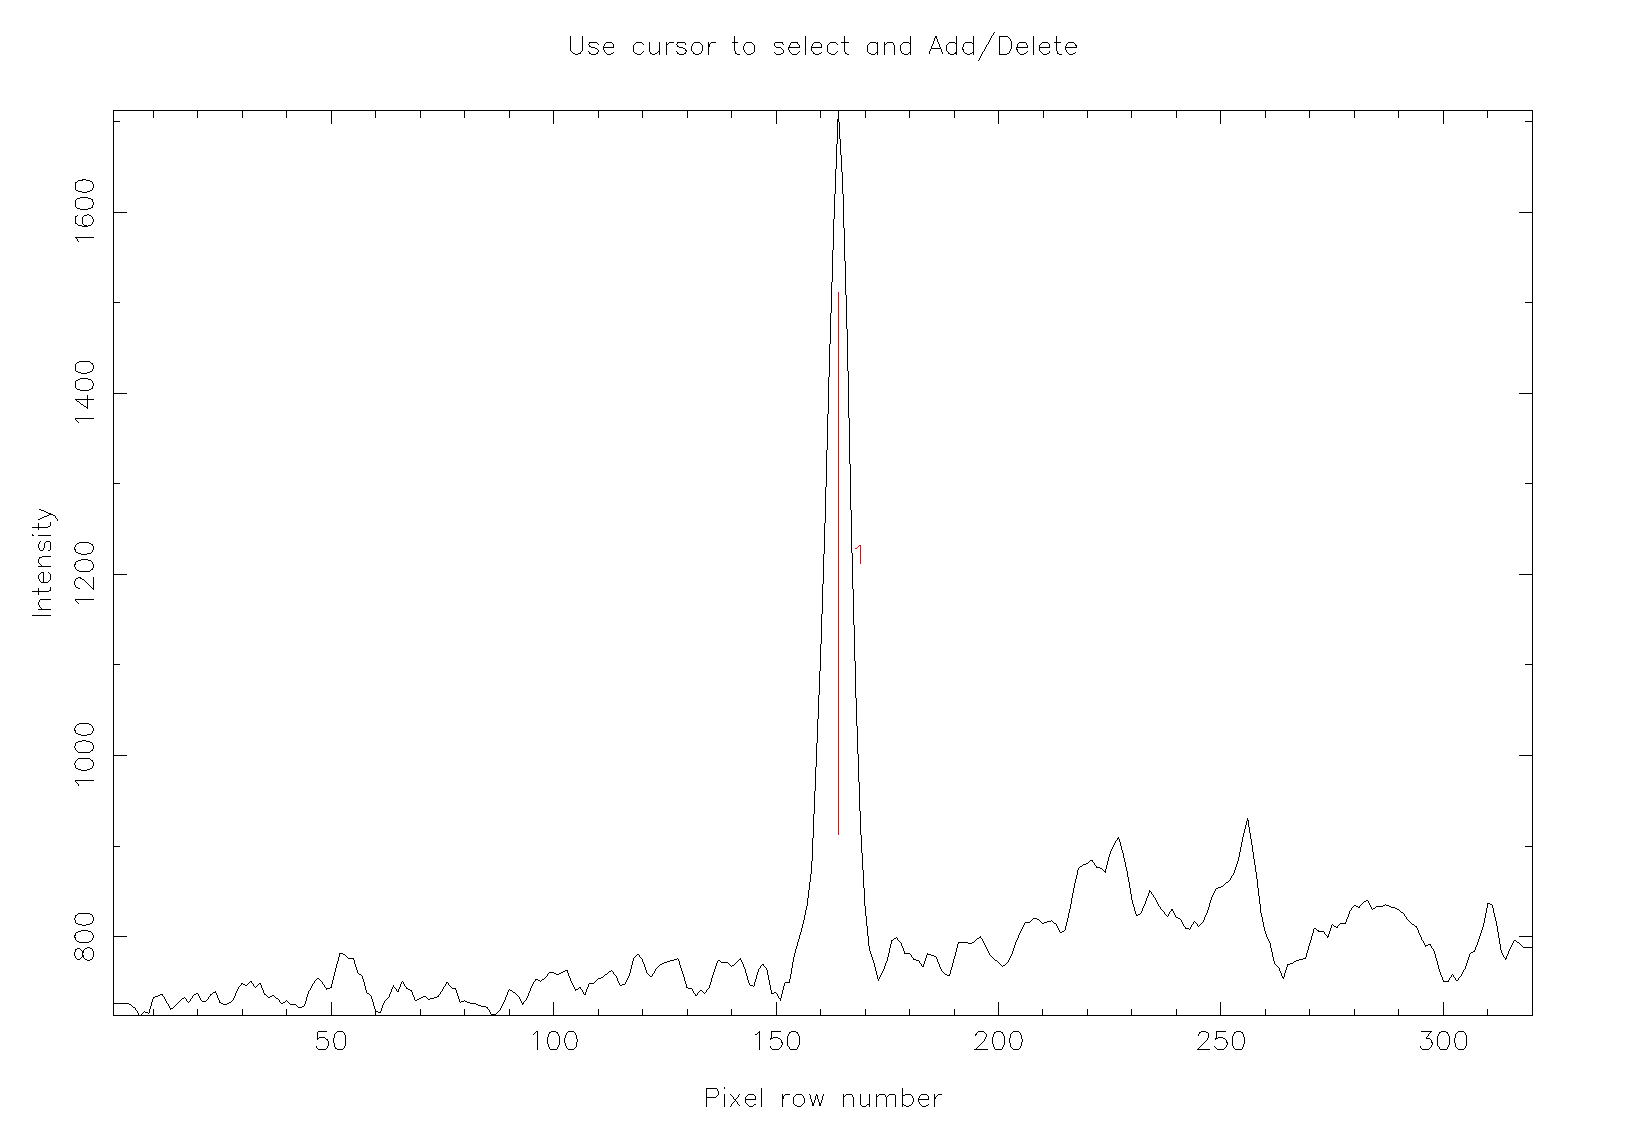
\includegraphics[height=136mm]{sc7_10}}

   \parbox{140mm}{
   \caption{Order location: a cross-dispersion section produced using
            {\bf echmenu} Option~1 {\sl Start a reduction.}}
   \label{fi_order_locate}
  }
\end{center}
\end{figure}

{\bf echmenu} now displays a slice across the image \verb+object+ and you
will see that it automatically locates features which look like they may be
spectra.  \scspec{Figure~\ref{fi_order_locate}}{The figure above} shows
such a plot.

A short menu of options is displayed, if (as in this case) all is well,
you can just hit the \verb+E+ key to accept the spectrum as correctly found.
You may find that {\bf echmenu} incorrectly guesses where the spectrum is;
you can use the \verb+C+ key to remove the automatically located spectra and
the \verb+A+ key to add a spectrum at the point indicated by the graphics
cursor.

You will notice that {\bf echmenu} appears to be able to handle more than
one spectrum in one image; this is the case\scspec{---}{ - }it can handle
multiple separate spectra ({\it{e.g.}} from a fibre spectrograph) and
multi-order spectra from \'{e}chelle spectrographs.  But we don't need to
know about that at the moment.


\subsection{Tracing the Spectrum}

Having located the spectrum, we now get another menu; this is in fact
a shortened version of the full menu with the `most-likely' choices at
the top of the list.
We want the \xref{second option {\sl Trace orders}}{sun152}{option2};
we only have one order but it works the same way.

{
\scspec{\small}{ }
\begin{verbatim}
    - Option number /'or Y for default=2'/ > 2
    ------------------------------------------------------------------------
    Starting processing task:     Trace orders.                  (ECH_TRACE)

   TRCFIT - Function for trace fitting /'POLY'/ >
   TRACE_MODE - Type of order tracing to use /'C'/ >
   TRC_NPOLY - Number of coeffs of trace-fit function /4/ >
    Processing order 1...
    Data range (user-specified) from     10.00 to  25005.00.
    Order 1 traced from X=0 to 1025, with a sample success rate of 100%
\end{verbatim}
}

The parameters here are:
\xref{{\tt{trcfit}}}{sun152}{par_TRCFIT} is the type of fit function to use,
\verb+poly+ is often fine, \verb+spline+ works in most other cases;
\xref{{\tt{trace\_mode}}}{sun152}{par_TRACE_MODE} determines which algorithm
is used to find the spectrum at each X-sample ({\it{i.e.}} along the
wavelength/dispersion axis), \verb+C+ means centroid and
usually works fine, other options include \verb+G+ for a Gaussian fit, and
\verb+B+ for a simple centre-of-gravity fit;
\xref{{\tt trc\_npoly}}{sun152}{par_TRC_NPOLY} selects the number of
fit parameters ({\it{i.e.}} the order of fit for a \verb+poly+) for
a \verb+spline+ you need more parameters (seven plus
number-of-knots, times two).

\begin{htmlonly}
\begin{figure}
\begin{center}
  \leavevmode\includegraphics[height=136mm]{sc7_05}
  \parbox{140mm}{
    \caption{Trace of a spectrum overlaid on the image.}
    \label{fi_order_trace_again}
  }
\end{center}
\end{figure}
\end{htmlonly}

You will see a line plotted overlaid on the image on the graphics device.
\scspec{(Much like Figure~\ref{fi_order_trace}, see
page~\pageref{fi_order_trace}.)}{(Similar to the plot above.)}
This shows the path of the trace as determined by
\xref{{\bf echmenu}}{sun152}{ECHMENU}\@.
Usually the trace works well; to inspect the fit we use
\xref{Option~3 {\sl Clip fitted traces}}{sun152}{option3}.
The only parameter you will be prompted for here is

{
\scspec{\small}{ }
\begin{verbatim}
    TRC_INTERACT - YES for interactive order-fitting /YES/ >
\end{verbatim}
}

\begin{figure}
\begin{center}
  \scspec{\leavevmode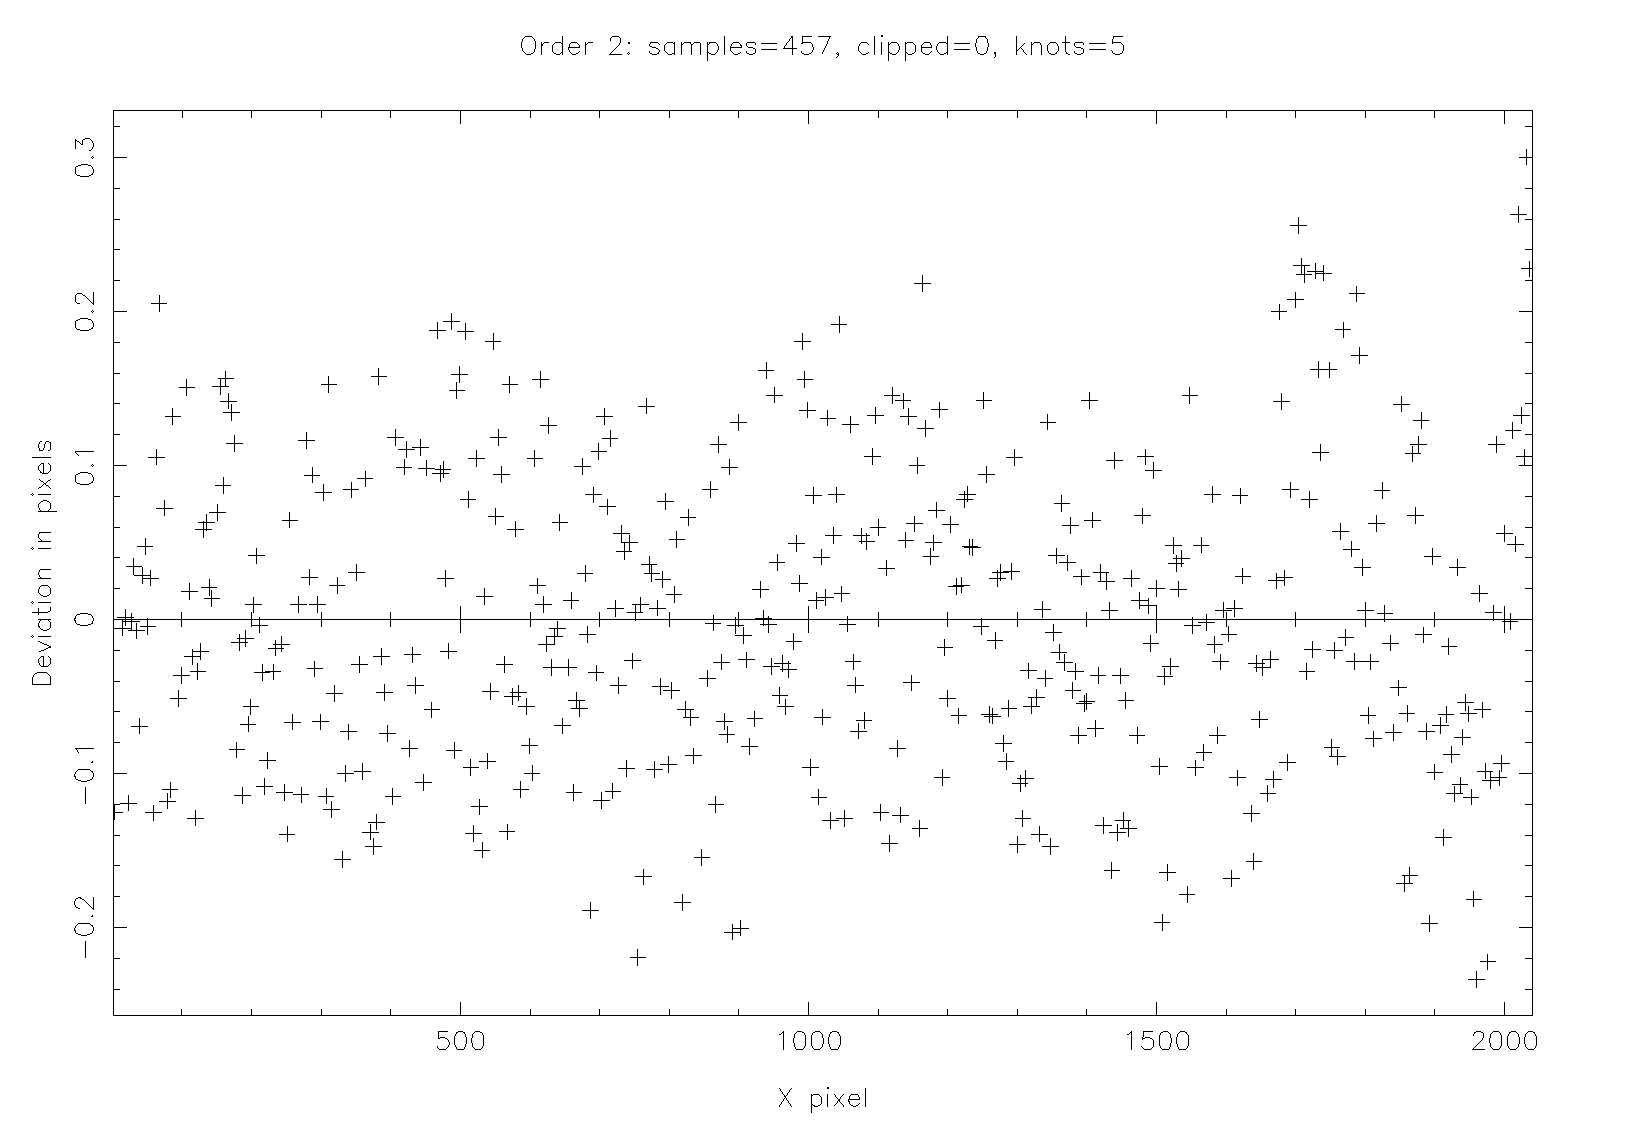
\includegraphics[height=100mm]{sc7_11}}
         {\leavevmode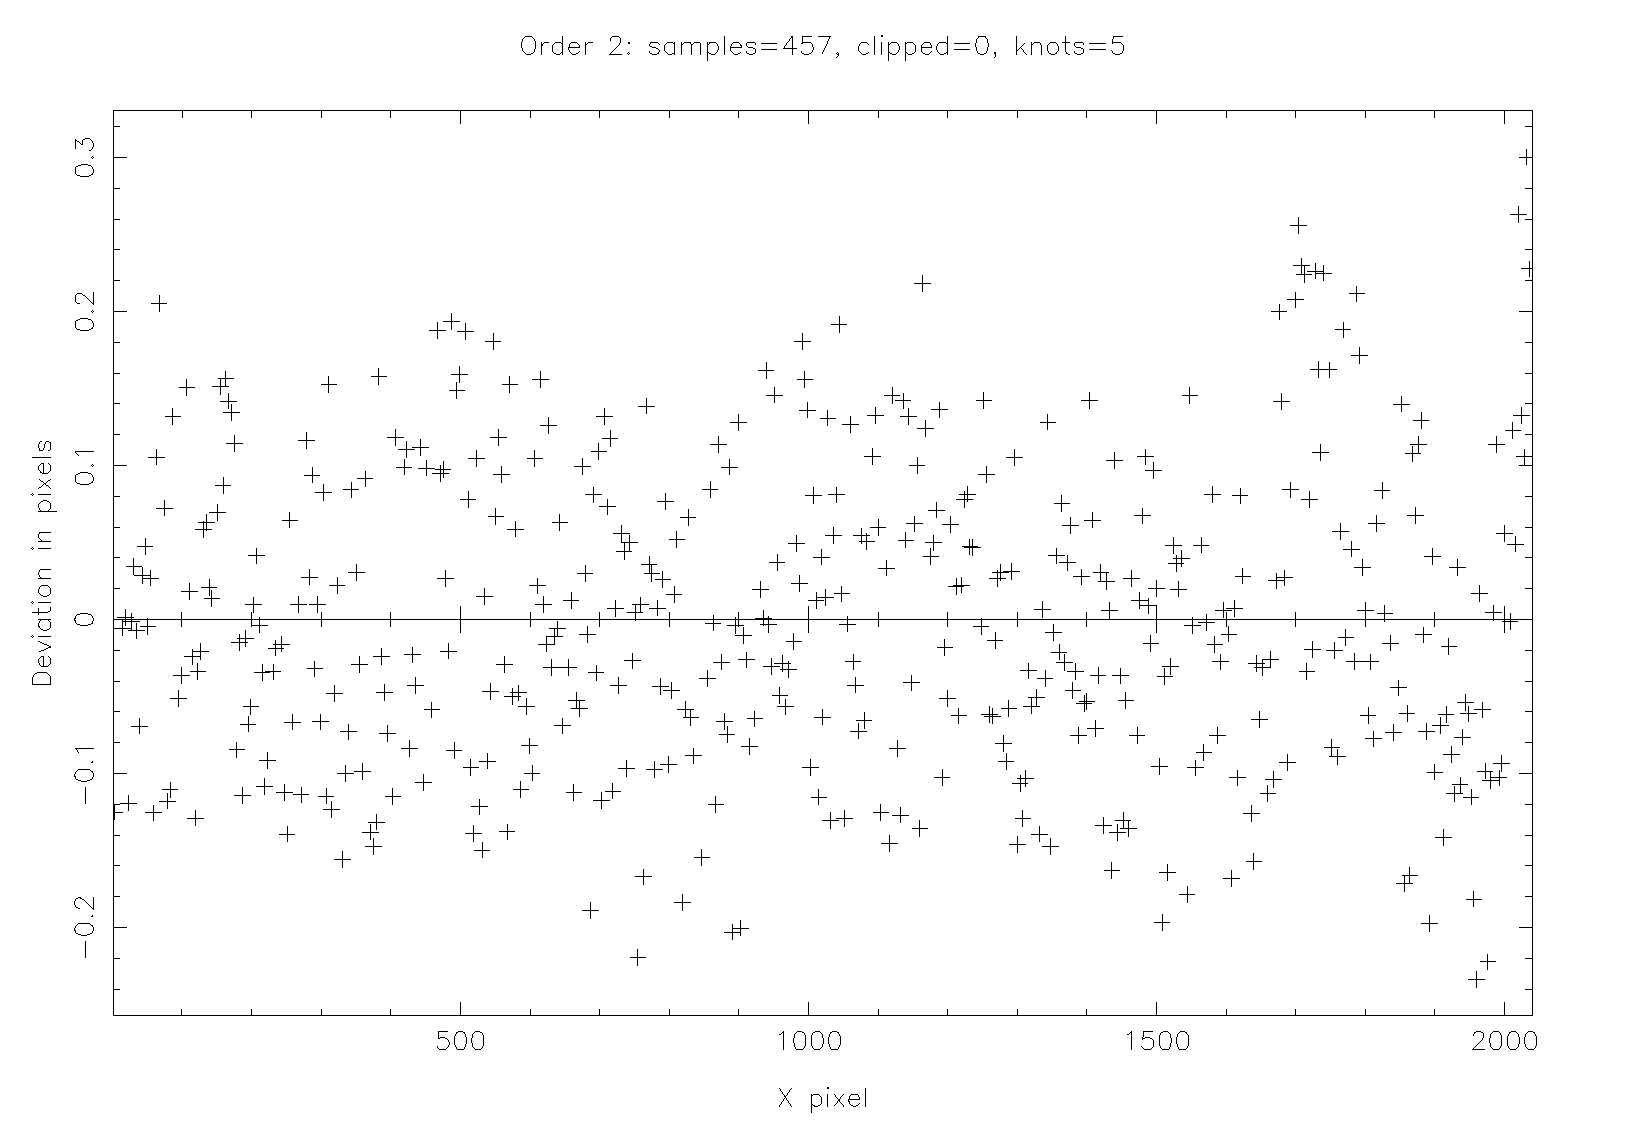
\includegraphics[height=136mm]{sc7_11}}

  \parbox{140mm}{
  \caption{Trace fitting: a display of traced points versus fitted trace,
           produced using {\bf echmenu} Option~3 {\sl Clip fitted
	   traces.} The plot is labelled `Order 2' as this was the
	   second order of an \'{e}chelle spectrum.}
    \label{fi_trace_fit}
  }
\end{center}
\end{figure}

Accept the default value (by hitting return) as we want to be able to
improve the trace interactively.
The first plot (see \scspec{Figure~\ref{fi_trace_fit}}
{the figure above}) shows the deviation of each X-sample in image
pixels from the trace path.
Values less than half a pixel are fine.  To see the
trace points plotted on the fitted trace curve hit the \verb+V+ key (the
full menu of options in the clipper can be displayed by hitting \verb+M+).
Hit \verb+V+ again to return to the `deviations' plot.  Deviant points can
be clipped in a number of different ways: use the \verb+.+ key to delete
the point closest to the graphics cursor; \verb+N+ clips points below the
cursor Y-position; \verb+P+ clips points above the cursor Y-position.
Option~\verb+R+ is often useful if part of the trace has gone wrong;
hit \verb+R+ to mark one end of the bad X-range and then hit the mouse
(usually left) button to mark the other end.
As points are clipped the display updates and the points
disappear\scspec{---}{ - }you should see the extent of the
deviations reduce.

When clipping, don't overclip\scspec{---}{ - }a nice `cloud' of deviations
of up to about plus or minus half of a pixel is fine.  If, when using a
\verb+poly+ curve you find that a very high-order fit (anything above 7th or,
perhaps 8th, order) is needed to get a good fit then you probably should
try a \verb+spline+ fit instead as you will start to `over-fit' the data.


\subsection{Choosing the Object and Background Channels}

The next step in the `data-modelling' process is to take a section through
the spectrum (cross dispersion) and decide which pixels contribute to the
object signal and which to the background.  The process is split into two
stages: first, deciding where the edges of the \htmlref{dekker}{gl_dekker}
are; second, choosing the channels.  Both stages are covered by
\xref{{\bf echmenu}}{sun152}{ECHMENU}
\xref{Option~4 {\sl Determine dekker/object extent}}{sun152}{option4},
they can be done separately as options 4.1 (dekker setup) and 4.2
(channel setup).

If you didn't specify \xref{{\tt
tune\_mxskypix=31}}{sun152}{par_TUNE_MXSKYPIX} when you started this
{\bf echmenu} session you should refer to
\scspec{\S\ref{cook_parameter_editor}}
{\htmlref{How to Use the {\bf echmenu} Parameter Editor}
{cook_parameter_editor}} for details of how to do this within
{\bf echmenu}\@.

The first prompts in Option~4 are:

{
\scspec{\small}{ }
\begin{verbatim}
   PFL_INTERACT - YES for interactive profiling /YES/ >
   SLITIM - Frame for dekker measurement /''/ > flat
\end{verbatim}
}

You should set
\xref{{\tt pfl\_interact}}{sun152}{par_PFL_INTERACT} to \verb+yes+
(or \verb+true+, means the same thing) as you may want to adjust the
dekker limits interactively.
\xref{{\tt{slitim}}}{sun152}{par_SLITIM} is the name of the image you
are going to use to find the edges of the slit; the object image will
do, but the flat-field image is often better as the flat-field has
steeper, and so clearer, edges.
Specify \verb+flat+ if you are working with the example dataset.

As in previous options, you will be presented with a displayed graph and a
short menu of options.  The graph shows a section across the dispersion
generated by averaging the cross-dispersion profile in some fraction
of the X-samples.  By default {\bf echmenu} uses the middle 20\% of the
pixels in the X-direction.
This gives a smooth(er) curve than a single-pixel section
and avoids the possibility of accidentally choosing a section across a
strong absorption feature.

\begin{figure}
\begin{center}
  \scspec{\leavevmode
\includegraphics[height=100mm]{sc7_12}}
         {\leavevmode
\includegraphics[height=136mm]{sc7_12}}

  \parbox{140mm}{
    \caption{Finding the dekker-limits of the slit: a plot of a section
             through a flat field, produced using {\bf echmenu} Option~4.1
             {\sl Determine dekker extent.}}
    \label{fi_dekker_limits}
  }
\end{center}
\end{figure}

In the plot (see \scspec{Figure~\ref{fi_dekker_limits}}{the figure above})
pixels which {\bf echmenu} has guessed as inside the slit are
displayed coloured
red\scspec{\footnote{The colours referred to will only be apparent if your
medium/display supports colour.}}
{(the colours referred to here will only be apparent if your
medium/display supports colour)}
and in a solid line; pixels outside the slit
are in green and a dot-dash line style.  To change the upper or lower
boundary, position the graphics cursor at the new dekker edge position,
and hit either the \verb+U+ key (upper limit) or \verb+L+ key (lower).
The new selection will be displayed.  If the profile appears to be wider
than the displayed graph then click a \verb+U+ or \verb+L+ with the
cursor outside the appropriate edge of the outline box and the display
will expand.  Once you are happy with the selection of the edges of
the dekker hit the \verb+E+ key.

\begin{htmlonly}
\begin{figure}
\begin{center}
  \leavevmode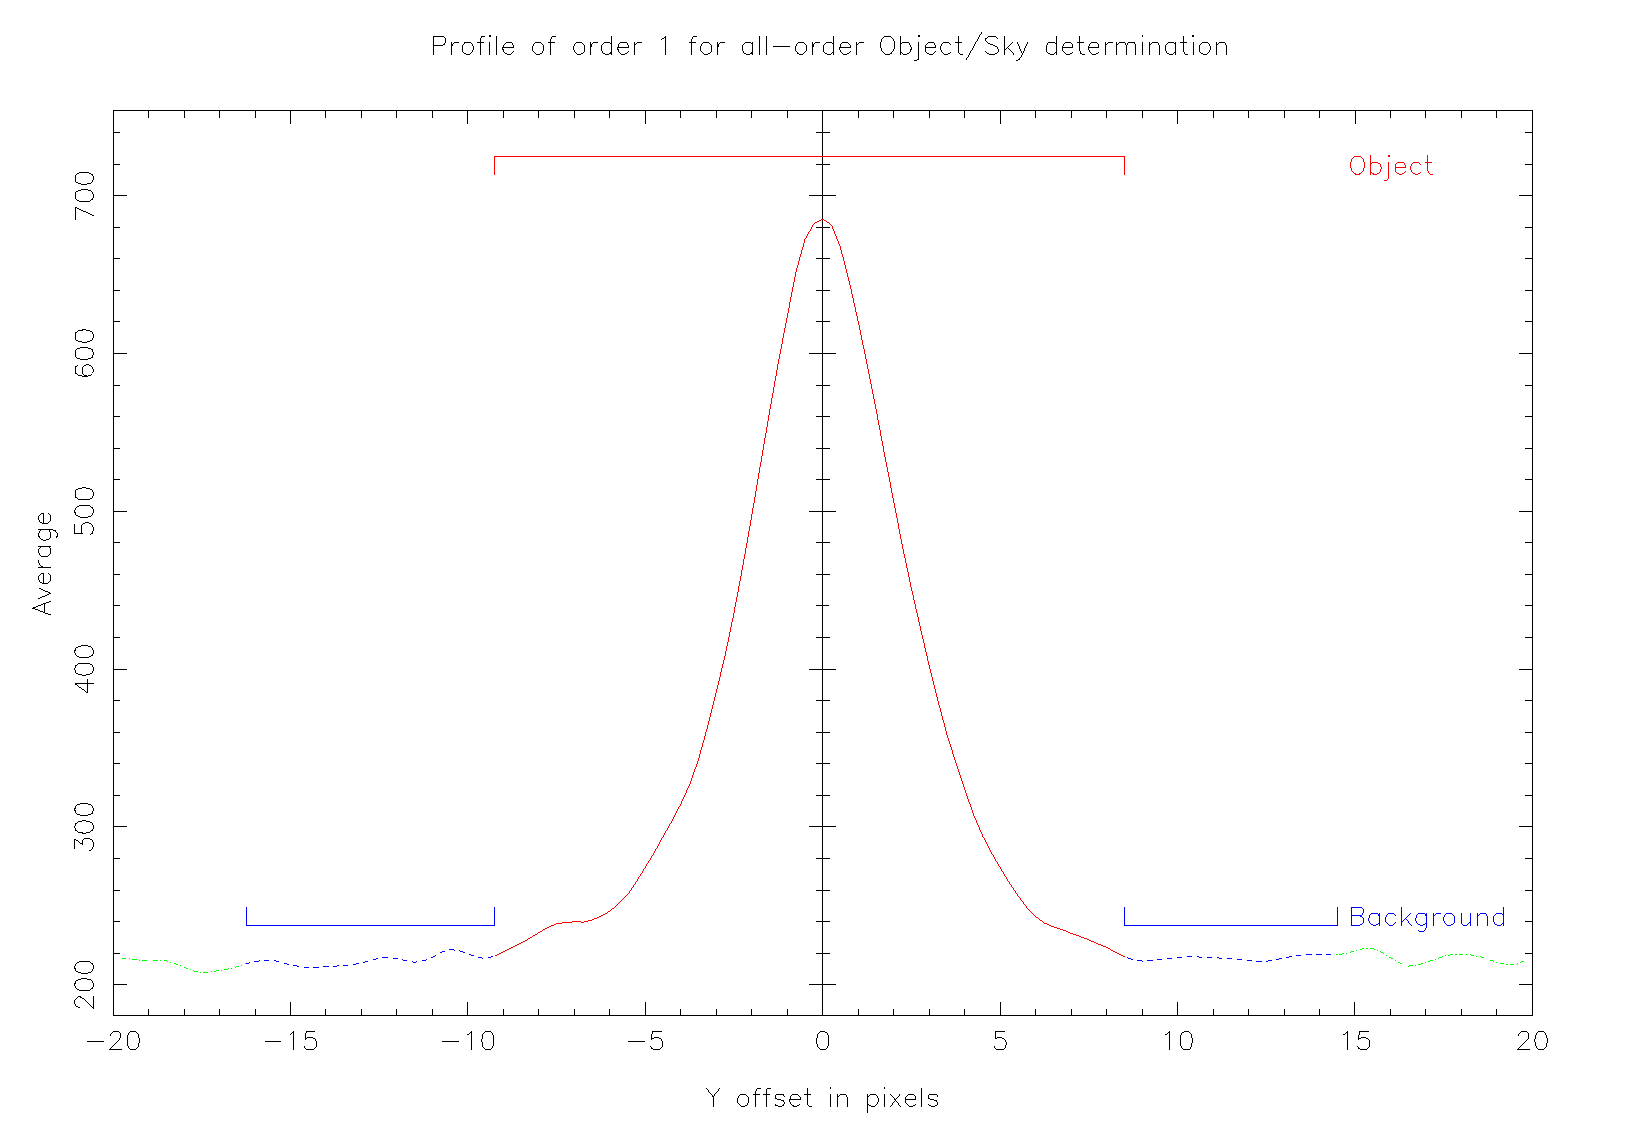
\includegraphics[height=136mm]{sc7_04}

  \parbox{140mm}{
    \caption{Selecting object and background channels: a plot of a section
             through an object spectrum, produced using {\bf echmenu}
             Option~4.2 {\sl Determine object limits.}}
    \label{fi_channel_select_again}
  }
\end{center}
\end{figure}
\end{htmlonly}

The next graph which pops up (such as
\scspec{Figure~\ref{fi_channel_select} (see page~\pageref{fi_channel_select})}
{the figure above}) is slightly more complex.  Once {\bf echmenu} has the
dekker limits it attempts to estimate which pixels within the slit are from
the object, and which are background (called sky pixels in {\sc echomop})\@.
In the plot, pixels chosen as object are shown in red and a solid line;
pixels selected as background are in blue and a dashed line;
pixels outside the dekker are again shown in green and a dot-dash line.
To help indicate the object and background channels, the pixels selected
are also marked with horizontal `brackets'; the object at the top (red);
the background at the bottom (blue).

At this point you should examine the profile carefully, looking for suitable
object and background channels.  It may be the case that the default
{\bf echmenu} settings automatically select good channels; however, better
results are often obtained by manually tweaking the selections.
You can still adjust the dekker limits at this point, again using the
\verb+U+ and \verb+L+ keys.
Use the \verb+S+ key to mark a particular pixel in the profile as background
(sky) and \verb+O+ to mark it as object.  If you are working with the example
datasets, try hitting \verb+S+ with the graphics cursor somewhere near the
middle of the profile; you will see the display update and a pixel will
change from object to background.  Click \verb+O+ to change it back to
object.

In the same way as in the \xref{trace-clipping option}{sun152}{option3}
you can use the \verb+R+ key
to start marking a range of pixels; press either \verb+O+ or \verb+S+ with
the graphics cursor at the other end of the range to mark the pixels as
object or background respectively.

You may have some pixels which appear to be neither object nor
background\scspec{---}{ - }perhaps there is some other object contaminating
the slit.  Use the \verb+I+ key to mark these pixels to be ignored, such
pixels appear in black, solid-line style on the plot.

At any point hitting the \verb+M+ key will display the full menu of options.
Hit the \verb+E+ key when the channels look sensible.  We now have the basic
parts of the model describing the data\scspec{---}{ - }a trace, and object
and background channels.


\subsection{Flat Fielding}

\xref{{\bf echmenu}}{sun152}{ECHMENU}
provides many options for flat fielding, these are handled by
\xref{Option~5 {\sl Model flat field}}{sun152}{option5}.

{
\scspec{\small}{ }
\begin{verbatim}
   FFIELD - Name of flat-field image /''/ > flat
   FLTFIT - Fitter for flat-field /'MEAN'/ > median
\end{verbatim}
}

There are only two prompts which appear at this point.
\xref{{\tt{ffield}}}{sun152}{par_FFIELD} is the name of our flat-field
image (in this case \verb+flat+) you can specify
\verb+none+ if you don't need flat fielding or have no image to use.
\xref{{\tt{fltfit}}}{sun152}{par_FLTFIT} is the type of model to fit
to the flat field.
We have selected \verb+median+ as this gives better rejection of deviant
data than \verb+mean+, which simply uses the average value over nearby
pixels to generate a smooth fit to the continuum lamp spectrum.
There are many other options, and the fit can be under interactive control.
A simple model is usually fine.


\subsection{Extracting the Spectrum}

The next stage in spectrum extraction is to model the background.
\xref{{\bf echmenu}}{sun152}{ECHMENU}
\xref{Option~6 {\sl Model sky}}{sun152}{option6}
performs the modelling and you can accept the default values for
the parameter prompts and get a reasonable model.
If you intend to perform optimal extraction you will need to find the
\xref{{\tt photon\_to\_adu}}{sun152}{par_PHOTON_TO_ADU} (gain) value and
\xref{{\tt readout\_noise}}{sun152}{par_READOUT_NOISE}\@.
You can do this using \xref{{\sc kappa}}{sun95}{}
\xref{{\bf fitslist}}{sun95}{FITSLIST}
to list the FITS extension in the input dataset, {\it{e.g.,}}
for the \verb+object+ in the example data:

{
\scspec{\small}{ }
\begin{verbatim}
   % kappa    # Only needed once per session.
   ... setup messages ...
   % fitslist object
\end{verbatim}
}

You should find the appropriate CCD parameters in the header, see
\scspec{\S\ref{cook_ccdchar}}
{\htmlref{Looking at FITS Header Cards: CCD Characteristics}{cook_ccdchar}}
for more details.  If the information you need is not present in the FITS
headers you will have to consult the observatory's CCD manual.

The only other data required prior to extraction is the profile model,
and this is only needed for optimal extractions.
{\bf echmenu} \xref{Option~7 {\sl Model object profile}}{sun152}{option7}
will generate a suitable model.
If you have been working through the example reduction data in a
single session, {\bf echmenu} will not prompt you for any further parameters
when you run Option~7.

And so to \xref{Option~8, {\sl Extract orders 1-D}}{sun152}{option8}.
The only new parameter for this option is

{
\scspec{\small}{ }
\begin{verbatim}
   EXTRACT_MODE - Extraction mode /'O'/ >
\end{verbatim}
}

The default value, \verb+O+, means optimal extraction.  Other options are:
\verb+S+ for a simple unweighted extraction, and \verb+P+ for a
profile-weighted extraction.


\subsection{Looking at the Extracted Spectrum}

\xref{{\bf echmenu}}{sun152}{ECHMENU} has an
\xref{Option (number 27)}{sun152}{option27}
for inspecting the contents of the current reduction database file.
You can start the option by typing \verb+P+ (for `plot') at the
main-menu prompt.
Once in the plotter, a menu appears and new prompt:

{
\scspec{\small}{ }
\begin{verbatim}
    - Option /''/ >
\end{verbatim}
}

\begin{htmlonly}
\begin{figure}
\begin{center}
  \leavevmode
\includegraphics[height=136mm]{sc7_07}
  \parbox{140mm}{
    \caption{An extracted spectrum.}
    \label{fi_extracted_spectrum_again}
  }
\end{center}
\end{figure}
\end{htmlonly}

If you type \verb+obj+ (for object) and then hit return, you will get a
plot of the extracted object spectrum (see
\scspec{Figure~\ref{fi_extracted_spectrum},
page~\pageref{fi_extracted_spectrum},}{the figure above} for an example).
You can get a list of things you
can plot by typing \verb+D+ (for directory).  Here's some of the ones which
might interest you at this stage:

\begin{latexonly}
\begin{center}
\begin{tabular}{llll}
 You type & You see & You type & You see\\ \hline
 {\tt SKY}  & Sky spectrum & {\tt SKYV} & Sky spectrum errors\\
 {\tt OBJ}  & Extracted object spectrum & {\tt OBJV} & Extracted object errors\\
 {\tt ARC}  & Extracted arc spectrum & {\tt FWAV} & Fitted wavelengths\\
 {\tt FFLT} & Fitted flat-field balance factors\\ \hline
\end{tabular}
\end{center}
\end{latexonly}
\begin{htmlonly}
\begin{verbatim}
   You type  You see
   SKY       Sky spectrum
   SKYV      Sky spectrum errors
   OBJ       Extracted object spectrum
   OBJV      Extracted object errors
   ARC       Extracted arc spectrum
   FFLT      Fitted flat-field balance factors
   FWAV      Fitted wavelengths
\end{verbatim}
\end{htmlonly}

We haven't generated the wavelength scale, so \verb+fwav+ isn't yet
available.

Another useful plotter option is \verb+L+ (limit X- and/or Y-range of plot).
You are prompted for the limiting values in both X- and Y-directions
(Y as plotted, rather than in the source image\scspec{---}{ - }so for
\verb+OBJ+, Y will be flux; for \verb+FWAV+, Y will be wavelength); enter
zero if any limit is to be determined from the data.

Once you have finished inspecting the spectrum, hit \verb+Q+ to return to
the main menu.


\subsection{\mlabel{example_wavelength_calibration}Wavelength Calibration}

There are two stages to \xref{{\bf echmenu}}{sun152}{ECHMENU}
wavelength calibration; the first stage is simple; the second stage may
be more complex.
The first step is to run
\xref{Option~9 {\sl Locate arc line candidates}}{sun152}{option9}\@.
This searches the arc spectrum for features which look like arc lines.
The result is a small list of potential features which can be used in
the second stage, wavelength calibration.

{\bf echmenu} \xref{Option~10 {\sl Identify features}}{sun152}{option10}
performs wavelength calibration.
There are a number of prompts:

{
\scspec{\small}{ }
\begin{verbatim}
   ECH_FTRDB - Reference line list database /'$ARCDIRS/THAR'/ > $ARCDIRS/CUAR
   ARC_TYPE - Type of arc lamp used /'$ARCDIRS/THAR.ARC'/ > $ARCDIRS/CUAR.ARC
   WAVFIT - Function for wavelength fitting /'POLY'/ >
   AUTO_ID - YES for fully automatic identification /FALSE/ >
   HI_WAVE - Longest wavelength to search for arc lines /0/ >
   LOW_WAVE - Shortest wavelength to search for arc lines /0/ >
   MAX_DISPERSION - Max dispersion (Units per pixel) allowed /1/ >
   MIN_DISPERSION - Min dispersion (Units per pixel) allowed /0.01/ >
   W_NPOLY - Number of coeffs of wavelength fitting function /7/ >
\end{verbatim}
}

Arc lamp database information for CuAr and ThAr lamps is available,
if you use some other lamp you will need a list of wavelengths for
features in the spectrum of the lamp.  Often a ThAr lamp is used,
however, in the example data the lamp used is CuAr,
so you can should set
\xref{{\tt ech\_ftrdb=\$ARCDIRS/CUAR}}{sun152}{par_ECH_FTRDB} and
\xref{{\tt arc\_type=\$ARCDIRS/CUAR.ARC}}{sun152}{par_ARC_TYPE}\@.
Note that the names of these files are case-sensitive.
\xref{{\tt{wavfit}}}{sun152}{par_WAVFIT} is the type of fit to use,
\verb+poly+ should be fine.

If you select
\xref{{\tt auto\_id=true}}{sun152}{par_AUTO_ID},
{\bf echmenu} will attempt a fully automatic wavelength calibration.
This will often work; however, it is better to
inspect the fit manually, rather than just accepting it automatically;
so we accept the default \verb+auto_id=false+\@.

\xref{{\tt hi\_wave}}{sun152}{par_HI_WAVE} and
\xref{{\tt low\_wave}}{sun152}{par_LOW_WAVE} are limits on the wavelength
range that might be covered by the spectrum; setting the limits both to
zero (the default) indicates we have no idea of the wavelength range.
However, if you do have a rough idea of either or both limits then enter
them here.
Constraining the wavelength range speeds up the process of feature
identification.
The units are Angstroms for the ThAr and CuAr databases.

\xref{{\tt max\_dispersion}}{sun152}{par_MAX_DISPERSION} and
\xref{{\tt min\_dispersion}}{sun152}{par_MIN_DISPERSION} are the limits on the
dispersion of the spectrum.  Again, if you know the dispersion, set these
values close to the value to help constrain automatic feature identification.
Inspection of FITS headers may reveal the dispersion used in your data,
you might otherwise look in the instrument handbook for the spectrograph
used.
The units here are Angstroms per detector pixel.  The default values are
set for common \'{e}chelle spectrographs and so may be too small for your
data.  If in doubt, set \verb+max_dispersion+ to a large value and leave
the default for \verb+min_dispersion+ as it is.

\xref{{\tt w\_npoly}}{sun152}{par_W_NPOLY} is the number of coefficients
of fit to use for the wavelength polynomial.
The default value of 7 is fine.
The fitter will adjust the order automatically the first time a fit is
made if the value is unusable.

\begin{htmlonly}
\begin{figure}
\begin{center}
  \leavevmode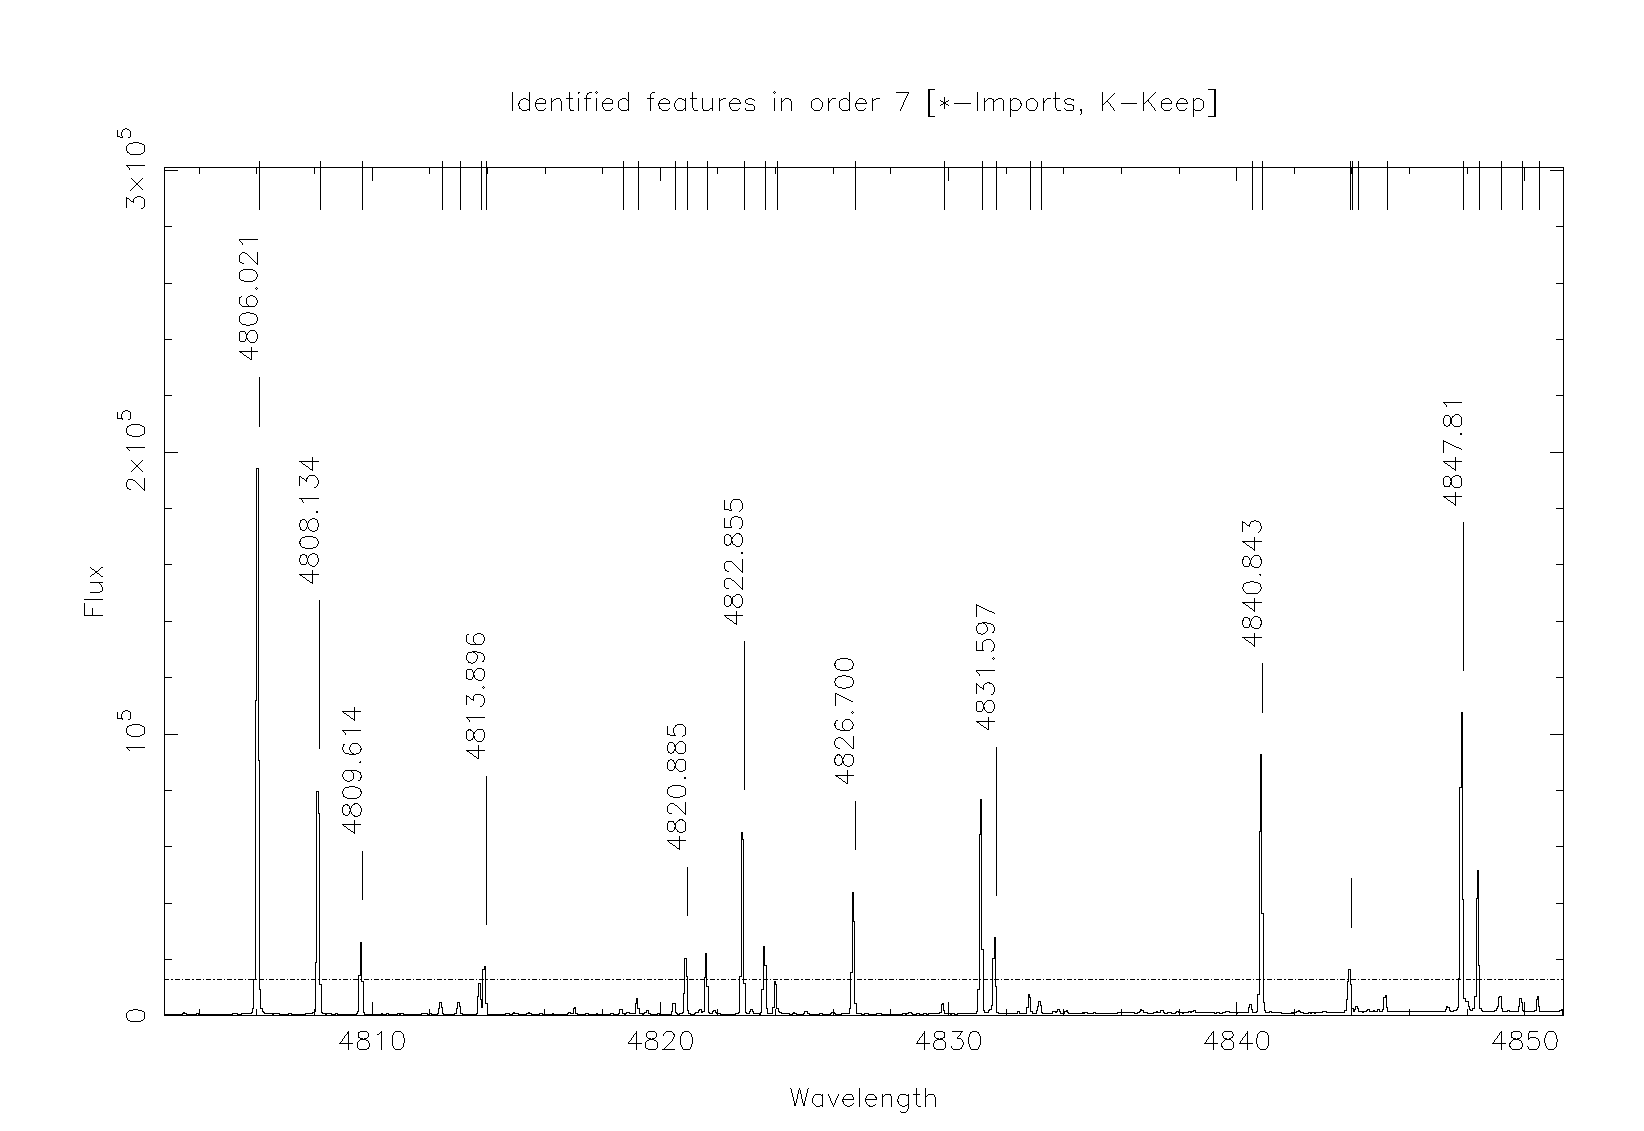
\includegraphics[height=136mm]{sc7_08}

  \parbox{140mm}{
    \caption{Line Identification: a typical plot during interactive fitting
             with \xref{{\bf echmenu}}{sun152}{}.}
    \label{fi_echarc_plot_again}
  }
\end{center}
\end{figure}
\end{htmlonly}

Once you have worked through all the prompts for Option~10 another mini-menu
will appear offering a default of \verb+I+ (identify features manually).
Accept the default by pressing return and (yet) another menu appears.  The
graphics display will also update showing the arc spectrum.  Each potential
feature identified in the arc spectrum will be marked by a short vertical
dash above the feature.  This will be similar-looking to
\scspec{Figure~\ref{fi_echarc_plot} (see page~\pageref{fi_echarc_plot})}
{the figure above,} except the features
will not yet be labelled with wavelengths.

All these sub-menus may appear confusing, however, you can just accept
the default to get to the interactive wavelength calibration.
The other options are used when the dataset is multi-spectrum or
multi-order.
You should now have a menu like this one:

{
\scspec{\small}{ }
\begin{verbatim}
    Option [Info,Del,Set,Thresh,Auto,New,Plot,Re-interp,Worst,BClip,Fit,+-=,
            XClip,Clear,Keep,List,Move,Zoom,Ozoom,>,<,Exit,Quit,Help,?]
\end{verbatim}
}

As you can see, there are rather a large number of options.  To apply an
option, type its first letter with the graphics cursor on the displayed plot.
Try an \verb+A+, which will attempt automatic calibration.  You will see
some details of the fit displayed and then a plot with the wavelengths of the
identified features overlaid.  For the example dataset this is all you
need to do\scspec{---}{ - }you now have a wavelength scale.
If the display zooms on to only a small part of the spectrum hit
\verb+R+ to get a full-spectrum plot.

At this point you may want to have one of the \htmlref{atlases}{atlases}
mentioned earlier to hand to check the identifications manually.
You can inspect the line-wavelength lists on-line, for example, the
ThAr list by:

{
\scspec{\small}{ }
\begin{verbatim}
   % more $ARCDIRS/THAR.ARC
\end{verbatim}
}

The important point in deciding whether the fit is good is the RMS error
of the fit.  Below is an example of a good fit:

{
\scspec{\small}{ }
\begin{verbatim}
              Line    Wavelength  Calculated Discrepancy    RMS if
                                  Wavelength                omitted

      1     297.366    4561.347    4561.349       0.001     0.00232
      2     451.861    4567.240    4567.238      -0.002     0.00243
    ... other lines ...
      9    1300.145    4598.763    4598.759      -0.004     0.00212
     10    1599.801    4609.567    4609.568       0.001     0.00207

    RMS error: 0.00250.

    Selected degree for fits: 4.
    Number of features identified: 10.
\end{verbatim}
}

You can see that the RMS error is quite small, also the `RMS if omitted
values' are all of similar values.  If a mis-identified or badly recorded
feature is included, then this will be indicated by a much lower
`RMS if omitted' than the other features.  To remove such a feature:
position the graphics cursor on the feature; hit \verb+D+ to delete the
feature from the list of features to be fitted; hit \verb+F+ to apply the
new fit.

It is important not to over-fit the feature list.  In the above example
ten points are fitted with a fourth-order curve; this is fine,
seventh-order would be too high as the errors would then be fitted away.
The plus and minus (\verb=+= and \verb=-=) keys change the order of fit.
Press the \verb+E+ key when you are happy with the fit.


\subsection{Normalising the Spectrum}

Once you have got the extracted, wavelength-calibrated spectrum you have
two options: you can output the data from {\sc echomop}; or, you can normalise
the spectrum to give a more-or-less flat continuum.  The next section
explains how to output data from {\sc echomop}.  This section outlines using
\xref{Option~11 {\sl Flatten order shape}}{sun152}{option11} to normalise
the data.

Enter \verb+11+ at the main \xref{{\bf echmenu}}{sun152}{ECHMENU} prompt
and the following parameter prompts will appear:

{
\scspec{\small}{ }
\begin{verbatim}
    FFIELD - Name of flat-field image /''/ > flat
    BLZFIT - Function for blaze fitting /'POLY'/ > spline
    BLZ_INTERACT - YES for interactive blaze-fitting /NO/ > Y
    BLZ_NPOLY - Number of coeffs of blaze fitting function /7/ > 28
\end{verbatim}
}

\xref{{\tt{ffield}}}{sun152}{par_FFIELD} is the name of the image to be
used to model the instrument profile, if you have been working through the
example data in one session you won't be prompted for this parameter
again.
You don't have to use a flat-field image; one option is to use
the object spectrum image itself and fit a curve to the continuum.
If you are following the example reduction, choose to use the flat-field
image \verb+flat+\@.
For modelling the instrument response a \verb+spline+ curve is often
better than a \verb+poly+, this is simply because it is unusual
for the response to be well represented by a simple polynomial, hence we
have chosen \xref{{\tt{blzfit=spline}}}{sun152}{par_BLZFIT}\@.
\xref{{\tt blz\_interact=y}}{sun152}{par_BLZ_INTERACT} selects
interactive adjustment of the fit.
\xref{{\tt blz\_npoly}}{sun152}{par_BLZ_NPOLY} sets the number of
parameters for the fit; we have chosen 28 as this is a \verb+spline+\@.
(Remember, for a spline we need seven plus number-of-knots, times two,
parameters.)

After entering values for the parameter prompts, you will see a display
very similar to that in the trace clipper; the same bit of code does both
jobs.  This means that you can use the same keys ({\it{e.g.}} \verb+V+, to
see the fitted curve versus the measured data) to view and improve the fit.
Use \verb=+= and \verb=-= to increase or decrease the order of fit; \verb+C+
to clip points further from the X-axis than the current graphics cursor
position.  Once you are happy with the fit, hit \verb+E+ to accept it.

At this point you can re-run
\xref{Option~27 (or {\tt{P}}, the plotter)}{sun152}{option27}
and view the flattened spectrum:

{
\scspec{\small}{ }
\begin{verbatim}
    - Option number /'or Y for default=1'/ > P
    ... messages ...
    - Option /''/ > OBJ
\end{verbatim}
}


\subsection{Output the Spectrum}

\xref{{\bf echmenu}}{sun152}{ECHMENU}
\xref{Option~14 {\sl Save reduced data}}{sun152}{option14}
handles the output of data.
You can produce NDFs which \xref{{\sc dipso}}{sun50}{}\cite{dipso},
\xref{{\sc kappa}}{sun95}{} and \xref{{\sc figaro}}{sun86}{} can read,
or you can output ASCII listings of the spectra.

{
\scspec{\small}{ }
\begin{verbatim}
   ECH_RDUCD - Output spectrum data file /'ECH_RDUCD'/ > spectrum
   RESULT_FORMAT - Output format required /'NDF'/ >
   RESULT_TYPE - Type of result output required /'EXTOBJ'/ >
\end{verbatim}
}

Here
\xref{{\tt ech\_rducd}}{sun152}{par_ECH_RDUCD} is the rather opaque-sounding
prompt for `output file name';
\xref{{\tt result\_format}}{sun152}{par_RESULT_FORMAT} is \verb+NDF+,
select \verb+ASCII+ for a listing instead;
\xref{{\tt result\_type}}{sun152}{par_RESULT_TYPE} should be set to
\verb+extobj+ to output the extracted spectrum, \verb+extarc+ to output
the extracted arc.

If you followed the example data reduction, you will now have a file
\verb+spectrum.sdf+ in the working directory which contains a normalised,
wavelength-calibrated spectrum which can be read by other Starlink
software.




%%%%%%%%%%%%%%%%%%%%%%%%%%%%%%%%%%%%%%%%%%%%%%%%%%%%%%%%%%%%%%%%%%%%%%%%%%%
\section{\mlabel{longslit_reduction_steps}Longslit (2-D) Data Reduction}
\markboth{Longslit Reduction Steps}{\stardocname}

In this section each of the basic steps in the longslit spectral data reduction
procedure are described. Many of the initial steps are similar to those
for 1-D data and reference will be made to those sections with notes
for any slight differences. Later steps do become 2-D data specific.

Examples of practical techniques using these ideas are to be found
in \scspec{\S\ref{longslit_worked_example}}
{\htmlref{A 2-D Worked Example}{longslit_worked_example}}.


\subsection{\mlabel{image_long_preparation}Image Preparation}

The essential basic difference with 2-D data is that we are not
looking to extract a region of the CCD frame into a single spectrum
but wish to preserve the spatial direction in order to study changes
in the spectrum with position.

Given this, the initial image preparation is the same as for 1-D data
which is described in \scspec{\S\ref{image_preparation}}
{\htmlref{{\sl Image Preparation}}{image_preparation}} and
 \scspec{\S\ref{flat_fielding}}
{\htmlref{Flat Fielding}{flat_fielding}}.



The order in which 2-D data is calibrated is different to that for 1-D
data. Many of the tasks in processing the data (e.g. background sky
emission line subtraction) require the 2-D frame to be correctly
oriented with spatial and dispersion axes perpendicular.

As can be seen in the example arc line image (see
\scspec{Figure~\ref{arc_line_curve},page~\pageref{arc_line_curve},}{the
figure below} for an example) the
lines have a definite curvature along the spatial axis. This is due to
the different path lengths the light takes through the optics along
the slit. Correcting for this is carried out along with wavelength
calibration.

\begin{figure}
\begin{center}
  \scspec{\leavevmode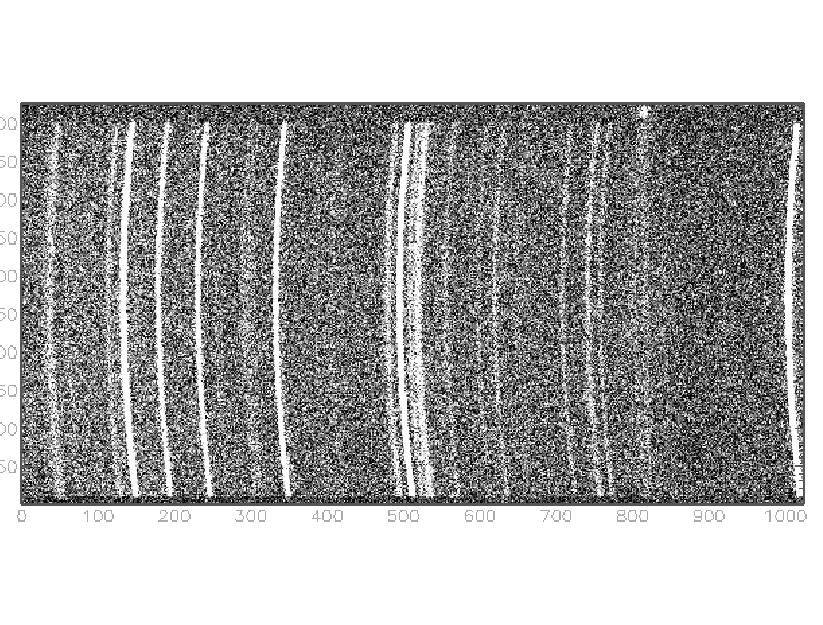
\includegraphics[height=105mm]{sc7_13}}
         {\leavevmode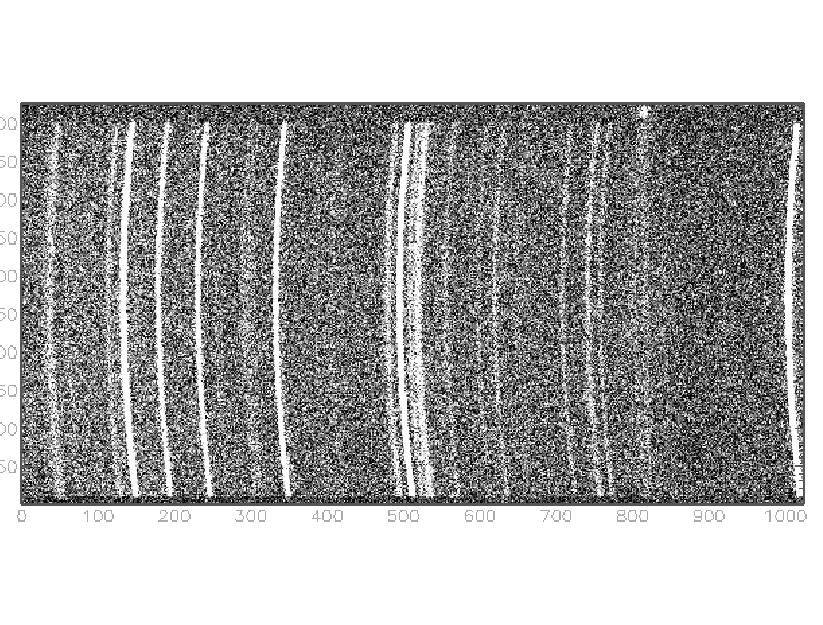
\includegraphics[height=136mm]{sc7_13}}

  \parbox{140mm}{
    \caption{A 2-D arc line image showing curvature along the spatial axis.}
    \label{arc_line_curve}
  }
\end{center}
\end{figure}




\subsection{\mlabel{arc_fit}Wavelength and curvature calibration}

The process of wavelength calibration along the dispersion axis also
allows us to correct for the geometric curvature of the frame
described above.

The wavelength calibration works in the same way as described for 1-D
spectra, matching the wavelengths of known arc lines to the pixel
values for the centres of the lines and performing a polynomial fit to
the data. Before this can be done we must calculate the curvature of the arc
lines on the frame in order to straighten them.

Both of these tasks are typically done by the fitting of Gaussian
functions to each arc line profile for each cross-section of the
frame. These then give the centre of each arc line for each
cross-section which can then be fitted by a polynomial along the arc
line. A polynomial matching pixel and wavelength values along the
dispersion axis can then be fitted.

For 2-D frames these fits are output in an .iar file, which contains
the polynomial coefficients. These can then be used by other programs
to 'scrunch' the data, in other words to resample the data correcting
the distortions and calibrating the wavelength axis.

As with 1-D spectra it is important to use arc lines which enable a
sensible polynomial fit to be made, i.e. well spaced over the whole of
the CCD. Similarly, as low an order polynomial as sensibly fits the
data should be used to prevent large errors being generated at the ends
of the dispersion axis.

\subsection{\mlabel{scrunching}Scrunching}

With the solution calculated for the calibration of the 2-D frame the
next stage is to apply this to the data. This process is called
scrunching.

The program (e.g. iscrunch in figaro) will take your .iar file
containing the solution and a data frame and apply the corrections and
calibration to it. This will involve re-binning the data and adding a
new wavelength axis.

It can also be a useful test to scrunch the original arc frame, which
should result in a set of perfectly straight arc lines.

A slightly more advanced program (iscruni in figaro) will allow you to
use two .iar files and use the average values when calibrating the
data. This is useful for long data exposures where arcs may show a
shift from arc line images taken before and after the data.


\subsection{\mlabel{fluxcal_2d}Flux calibration}

Flux calibration works in much the same way as for 1-D spectra, see
\scspec{\S\ref{flux_calibration}}
{\htmlref{{\sl Flux Calibration \&
               Extinction Correction}}{flux_calibration}}.

The only difference comes when applying the calibration to the data
when each row of the 2-D frame is calibrated rather than a simple
spectrum.



%%%%%%%%%%%%%%%%%%%%%%%%%%%%%%%%%%%%%%%%%%%%%%%%%%%%%%%%%%%%%%%%%%%%%%%%%%%
\section{\mlabel{longslit_worked_example}A 2-D Worked Example}
\markboth{A 2-D Worked Example}{\stardocname}

As there may be readers who have come to this section without reading
the worked 1-D example I will reiterate a number of instructions. If
you are familiar with the early steps please feel free to skip on.

Before you start the extraction you will have to do the
detector-specific preparation of your data (most likely to remove
CCD-related effects).
If you have not done this, refer to \scspec{\S\ref{image_preparation}}
{\htmlref{Image Preparation}{image_preparation}} for an outline of the
procedure, and \scspec{\S\ref{other_sources}}
{\htmlref{Other Sources of Information}{other_sources}} for pointers
to documentation of the process.


\subsection{Setting Up}

The first thing you need to do (if you've managed to prepare your CCD
data you will most likely know this already, but\ldots ) is to run the
Starlink setup.
Normally Starlink software is installed in the \verb+/star+ directory
and the commands you must execute are:

{
\scspec{\small}{ }
\begin{verbatim}
   % source /star/etc/cshrc
   % source /star/etc/login
\end{verbatim}
}

If your Starlink software is installed somewhere else,
then modify the commands appropriately.
Most people include these lines in their shell login file
(\verb+.login+ in your home directory).

Once you have done the Starlink `login' you can initialise for any of the
major packages simply by typing their names.
For example, we are going to use
\xref{{\sc figaro}}{sun86}{}\cite{figaro}, \xref{{\sc kappa}}{sun95}{}\cite{kappa} and
\xref{{\sc twodspec}}{sun16}{}\cite{twodspec} and so get a display
something like:

{
\scspec{\small}{ }
\begin{verbatim}

   % figaro     # Only needed once per session.

 ----------- Initialising for  Figaro ------------
              General data reduction
            Version 5.3-0  29 December 1997

          Type "fighelp figaro" for help
      or "fighelp news" for news on changes

 Type "showme sun86" to browse HTML documentation

 Use "abbrev" and "noabbrev" to turn parameter name
 abbreviation on and off.


   % kappa    # Only needed once per session.

      KAPPA commands are now available -- (Version 0.9-3)
      KAPPA uses NAG routines, by permission of NAG ltd.

      Type kaphelp for help on KAPPA commands
      Type "showme sun95" to browse the hypertext documentation


   % twodspec   # Only needed once per session.

   TWODSPEC commands are now available -- (Version 0.9-0)

   Type "showme sun16" to browse the hypertext documentation.
\end{verbatim}
}

We can now use {\sc figaro}, {\sc kappa} and {\sc twodspec} commands.

As with the 1-D example, you might like to take a copy of the example
data which comes with this document when installed as part of the
Starlink document set. You will find the files in the directory

{
\scspec{\small}{ }
\begin{verbatim}
   /star/examples/sc7/
\end{verbatim}
}

Create an empty directory and enter it using \verb+cd+\@.
To copy the test data type the command

{
\scspec{\small}{ }
\begin{verbatim}
   % /star/examples/sc7/copy2ddata
\end{verbatim}
}

You will then find you have these data files in your directory:

\begin{latexonly}
\begin{center}
\begin{tabular}{ll}
File & Description \\ \hline
{\tt object2d.sdf}  & Frame with the object spectrum\\
{\tt arcframe2d.sdf}     & Frame with a wavelength-reference arc\\
{\tt quartz2dscrun.sdf}    & Frame with a quartz lamp flat field\\
\end{tabular}
\end{center}
\end{latexonly}
\begin{htmlonly}
\begin{verbatim}
   File         Description
   object2d.sdf   Frame with the object spectrum
   arcframe2d.sdf      Frame with a wavelength-reference arc
   quartz2dscrun.sdf     Frame with a quartz lamp flat field
\end{verbatim}
\end{htmlonly}

\subsection{Inspecting the 2-D images}

At this stage it is assumed that the image files have been de-biased and
cosmic ray cleaned.

The first thing to do is to put the image frames on display for inspection.
This can be done using \xref{{\sc kappa}}{sun95}{}
\xref{{\bf display}}{sun95}{DISPLAY}:

{
\scspec{\small}{ }
\begin{verbatim}
   % idset xwindows
   % display object2d clear mode=pe accept
\end{verbatim}
}

This shows the data frame with two emission lines, in this case from
the Honeycomb Nebula in the Large Magellanic Cloud.  (see
\scspec{Figure~\ref{fi_twod_spectrum},
page~\pageref{fi_twod_spectrum}}{The figure in the introduction}).

The arc line image can be shown using:

{
\scspec{\small}{ }
\begin{verbatim}
   % display arc2d clear mode=pe accept
\end{verbatim}
}

The curvature of the arc lines, which we wish to correct, is obvious
(see \scspec{Figure~\ref{arc_line_curve},
page~\pageref{arc_line_curve}}{the previous figure}.

There are three key elements to the inspection of the images at this stage,

\begin{description}

\item [Check for rotation]
      Typically done by visual inspection or taking cuts through a
      continuum source (e.g. a star on the slit) in the object frame.

\item [Check the wavelength direction]
      Wavelength must increase from left to right and is checked by
      spotting known arc or observed line patterns.

\item [Noting the range of y-axis values over which the arc lines are seen]
      This is so that we know the sensible range over which to try and fit the arc lines.

\end{description}


These frames are correctly rotated (i.e. have the wavelength axis
parallel to the x-axis) and have wavelength increasing to the right.
If this is not the case with your data, methods for correcting this
were detailed previously in \scspec{\S\ref{inspecting_the_images}}
{\htmlref{Inspecting the Image}{inspecting_the_images}}.

With the arc line image displayed we can carry out the third item
mentioned above, noting the range of y-axis values the arc lines
extend over. To do this we can use the \xref{{\sc kappa}}{sun95}{}
\xref{{\bf cursor}}{sun95}{CURSOR} command:


{
\scspec{\small}{ }
\begin{verbatim}
   % cursor
\end{verbatim}
}

The cursor should then be placed at each end of an arc line and the
left mouse button clicked. This will report the coordinates of the
point in the terminal window. When this has been done click the right
mouse button to exit.

When I did this I obtained these values:

{
\scspec{\small}{ }
\begin{verbatim}
Picture comment: KAPPA_DISPLAY, name: DATA, reporting: PIXEL coordinates
 p1 = 144.6 (pixel)   p2 = 12.9 (pixel)
 p1 = 149.8           p2 = 492.7
\end{verbatim}
}

So we have a range of 13 to 493 in the y-axis.

We can now go on to the fitting of these arc lines.

\subsection{Arc line fitting}

To carry out the fitting we use the \xref{{\sc twodspec}}{sun16}{}
command {\tt arc2d}. This program provides a number of menus and
interactive displays and will be described in the text.


{
\scspec{\small}{ }
\begin{verbatim}
   % arc2d arcframe2d

arcframe2d[1024,525] THAR FOR PREV
Results structure present

=========< A r c _ O p t s >=========

New      : Set up line identifications from scratch
Repeat   : Use existing line identifications
Clone    : Use line identifications from another file
ARC_OPTS - Enter arc fit option /'ne'/ >

\end{verbatim}
}

We wish to carry out a new identification of the arc lines so type
{\tt new} and press return. The program will ask for confirmation of
this action, enter {\tt y} to the questions.

{
\scspec{\small}{ }
\begin{verbatim}
MAXLINES - Maximum number of lines to allow room for /5/ >
\end{verbatim}
}

This question asks for the number of arc lines you wish to use.
Ideally you would like a number of lines spread evenly over the CCD
array. As the resulting fits are typically 3rd order or lower then 5
lines is a reasonable default. Press return.

{\scspec{\small}{}
\begin{verbatim}
YSTART - analysis lower limit /20/ > 13
YEND - analysis upper limit /40/ > 493
\end{verbatim}
}



In order to identify the arc lines we have to select them
interactively. These question ask for the range of y-axis values over
which to extract a spectrum for this identification. Simply enter the
values which we found using the cursor earlier.

At this point the extracted spectrum will be displayed on the graphics
window. You will see that the lines are quite broad as we have summed
the data over a range in the y-axis and hence in curvature of the
line.

The lines are then selected using the mouse, going from left to right
across the spectrum in increasing wavelength. To select the lines to
be used the left mouse button is clicked to the left and right of the
arc line to mark tramlines. Only one arc line should lie within the
tramlines and there should be some continuum left on each side of the
line in order to fit a good baseline (see
\scspec{Figure~\ref{arc_select}, page~\pageref{arc_select}}{the figure
below.})


\begin{figure}
\begin{center}
\scspec{\leavevmode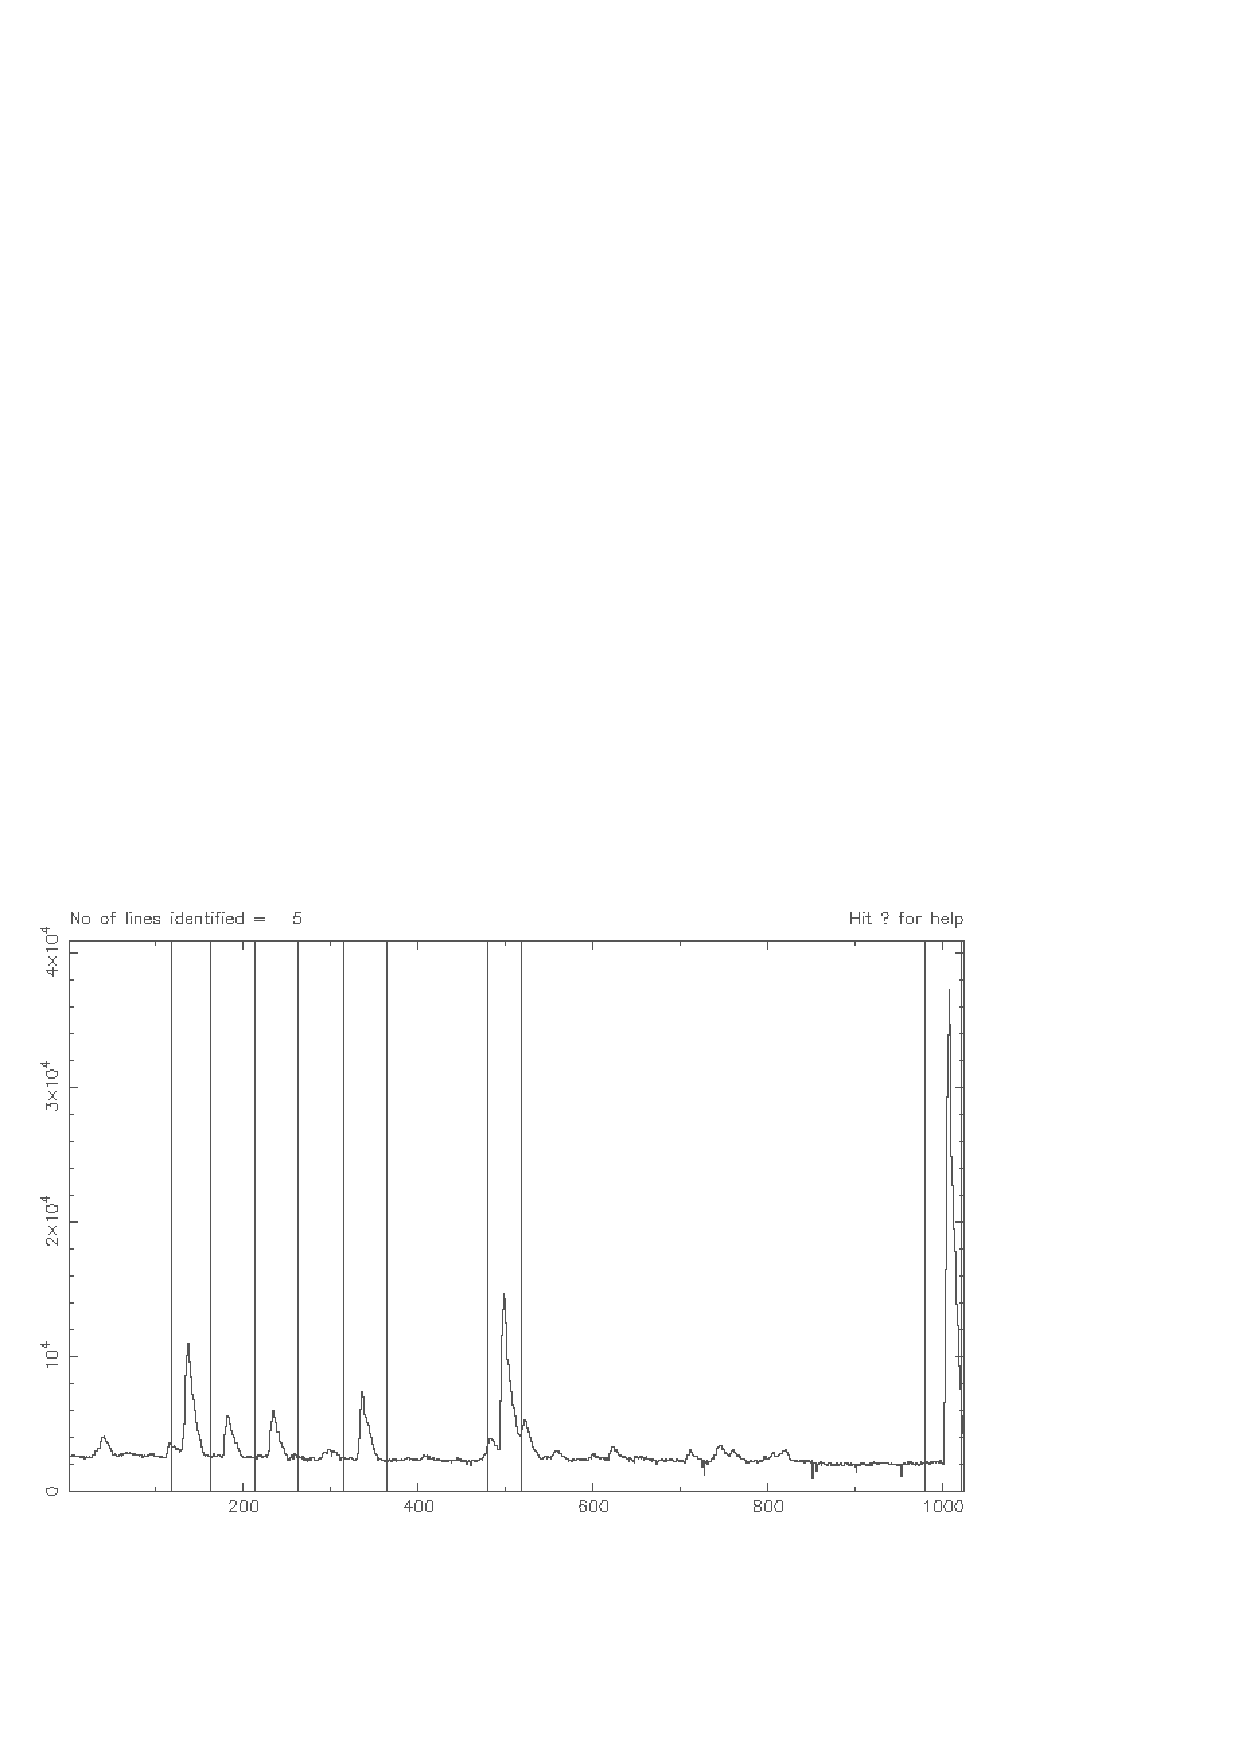
\includegraphics[height=105mm]{sc7_14}}
       {\leavevmode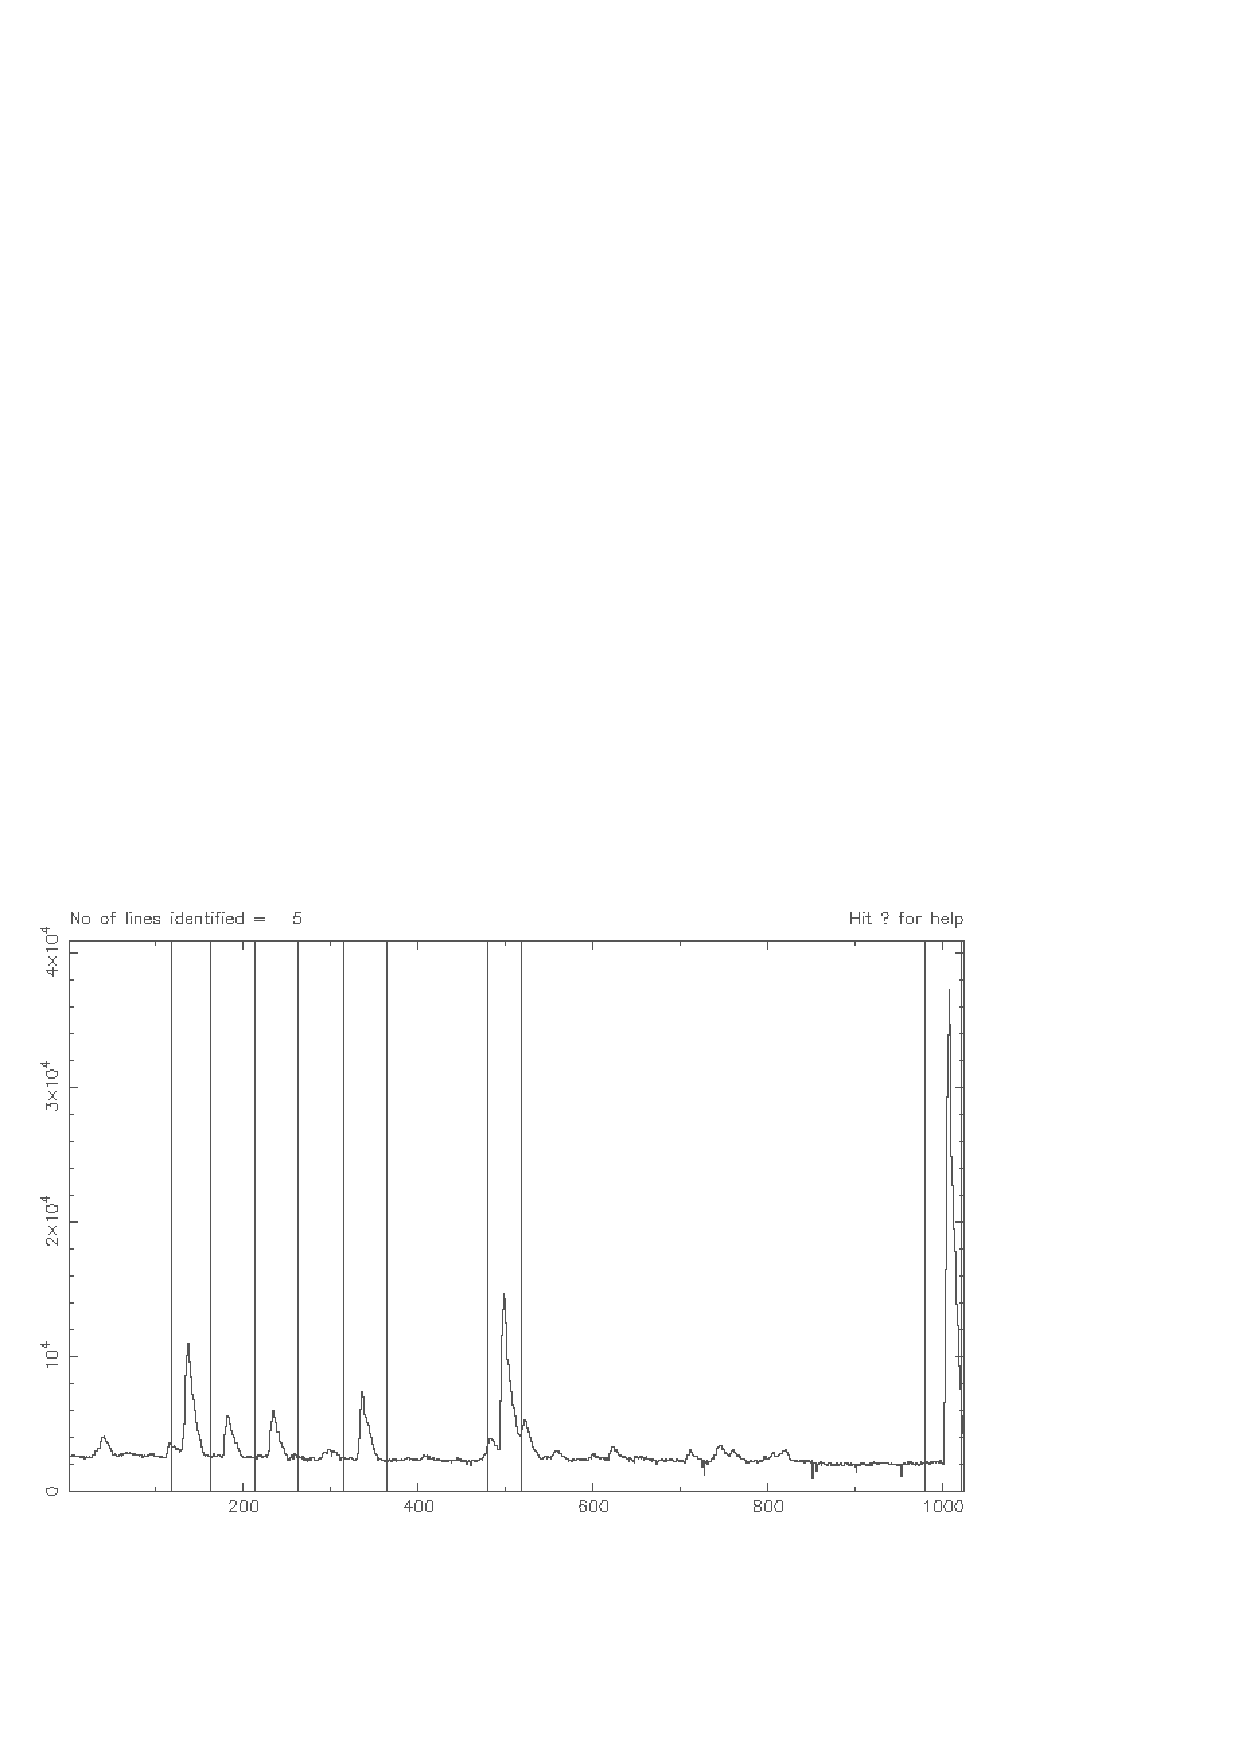
\includegraphics[height=136mm]{sc7_14}}

  \parbox{140mm}{
    \caption{An arc line spectrum with lines selected between the
             tram-lines.}
    \label{arc_select}
  }
\end{center}
\end{figure}

%FIGURE arclines.eps

\subsection{Arc line identification}

Once you have marked out each of the arc lines you wish to use press
{\tt e} to exit this stage. You are now given the option of selecting
a line list, simply a text file of known lines for particular arc
lamps or emission lines. These can be used as a reference when
identifying the selected lines. In this case the arc was a Thorium
Argon lamp for which a list is not available. The lines will then have
to be identified using an arc line catalogue.
\goodbreak

{\scspec{\small}{ }
\begin{verbatim}
=========< L i n e   L i s t   M e n u >=========

Emission   : Emission lines
Absorption : Absorption lines
Neon       : Neon arc
Cuar       : Copper-argon arc
Helium     : Helium arc
Iron       : Iron arc
SKy        : Sky lines
STored file: User supplied list in file
Ok         : All tables read in
\end{verbatim}
}

So we can type ok at this prompt.

The program now displays the first selected line in more detail and
prompts you for an identification on the terminal screen.

{\scspec{\small}{ }
\begin{verbatim}
L I N E   I D E N T I F I C A T I O N
-------------------------------------
Identify line number  1

=========< I d e n t i f i c a t i o n   M e n u >=========

[number]               : Line wavelength
Width [number]         : Redraw with different width
Next                   : Go to next line
Display                : Start/stop displaying line tables
Id [wavelength] [name] : Give line ID/wavelength
Quit                   : Exit leaving lines unidentified

\end{verbatim}
}

As we have found the arc line pattern in the catalogue we can enter
the known wavelengths for each arc line. The first line has a
wavelength of 6708.97 angstroms and so we enter

{\scspec{\small}{ }
\begin{verbatim}
id 6708.97 line1
\end{verbatim}
}
and then confirm this is correct.

The second line is now displayed and we similarly enter the wavelength
for this line. The wavelengths for the five lines marked in
\scspec{Figure~\ref{arc_select}}{the figure above}) are:

{\scspec{\small}{ }
\begin{verbatim}
id 6708.97 line1
id 6711.34 line2
id 6713.97 line3
id 6719.20 line4
id 6752.83 line5
\end{verbatim}
}

After this the program will display the entered list of
identifications for you to check. Enter no to 'edit line list' to
reach the main menu:

{\scspec{\small}{ }
\begin{verbatim}
=========< M a i n   M e n u >=========

Look : Look at values of data cube
Soft : Produce soft-copy plots of diagnostics
Hard : Produce hard-copy plots of diagnostics
Tols : Apply tolerances
Exit : Leave the program
Disp : Evaluate dispersion relation
Gaus : Fit Gaussians to line profiles
Add  : Add more lines
Poly : Fit polynomials in X-Sect direction
\end{verbatim}
}

\subsection{Curvature correction}

So we now have the lines identified with their wavelengths. The next
stage is to fit a Gaussian to each arc line for each row of the image.
The centres of these Gaussians will then be used to calculate the
corrections required.

Fitting these Gaussians is selected by entering {\tt gaus} at the main
menu prompt. Again we are asked for the limits over which rows the
program should try and fit Gaussians to the data. These should be the
same limits as you entered earlier, and the program will suggest these
values as defaults. The next question regards the blocking factor.
There is cost in processing time depending on how many Gaussians you
fit and one way to reduce this is to add a block of rows together.
Typically a blocking factor of 4 percent of the total number of rows
is reasonable, so for our case a value of 18 pixels. This value is not
crucial, so long as it is not larger then any obvious distortion in
the arc line across the CCD. Blocking also brings a benefit in that it
will increase the signal to noise ratio of the data and is often
essential in getting a good fit to low signal arc lines.

Enter {\tt 18} and press return. The next question asks if you wish to
see the Gaussian fits as they are carried out. If this is the first
time you have done this you may want to say yes, but experienced users
might say no as typically the fits are not very exciting and do take
some time to go through. An example Gaussian fit is shown in
\scspec{Figure~\ref{arclinefit}, page~\pageref{arclinefit}} {the
figure below}.

\begin{figure}
\begin{center}
  \scspec{\leavevmode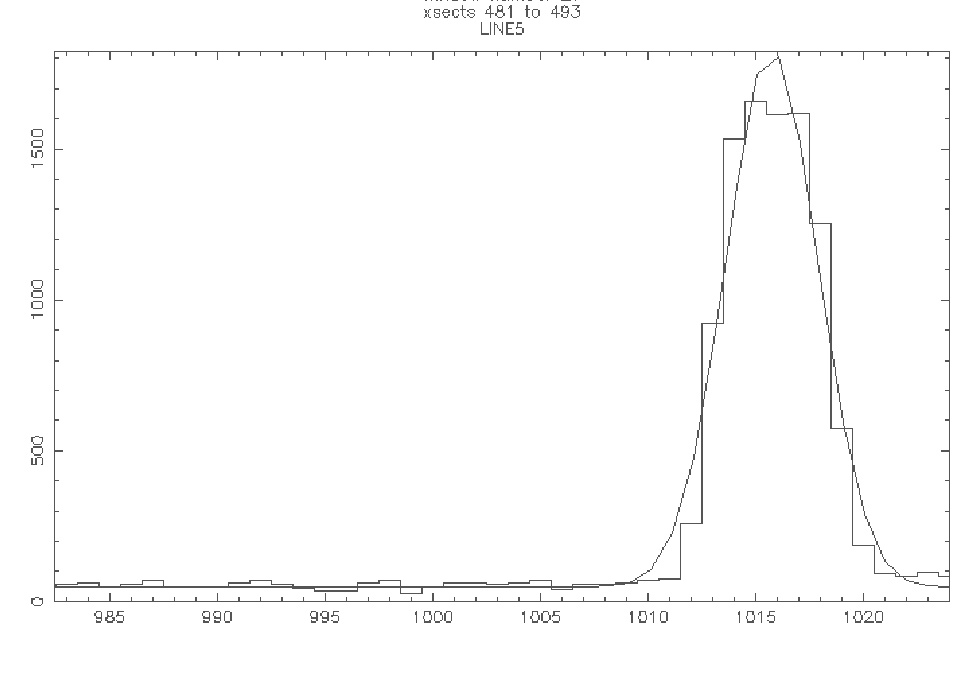
\includegraphics[height=105mm]{sc7_15}}
         {\leavevmode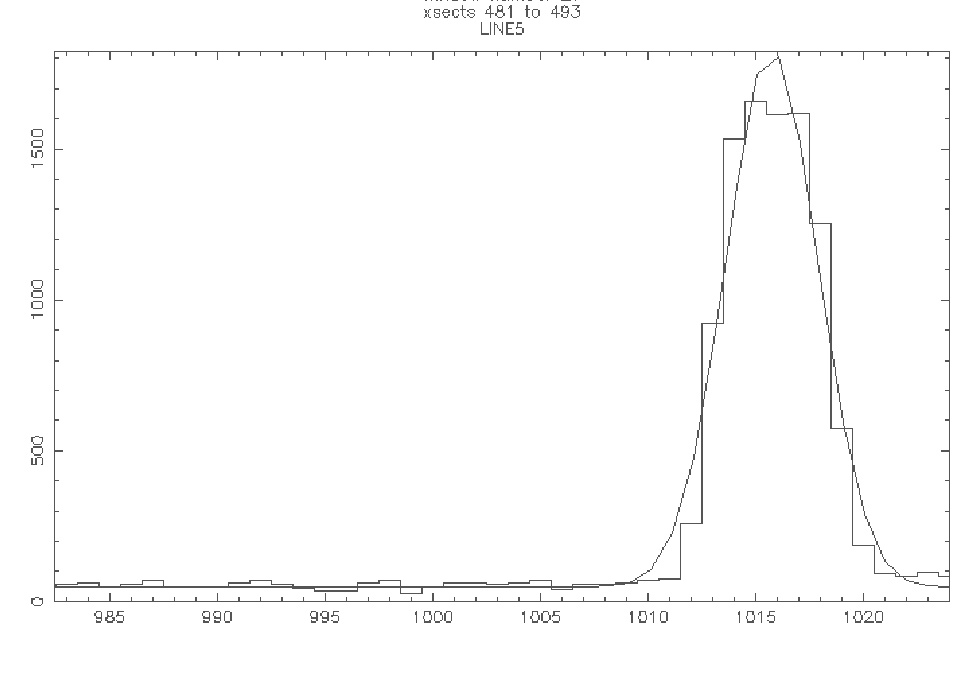
\includegraphics[height=136mm]{sc7_15}}

  \parbox{140mm}{
    \caption{An example Gaussian fit to an arc line spectrum.}
    \label{arclinefit}
  }
\end{center}
\end{figure}


After this has been completed you are returned to the main menu. With
the Gaussians fitted the next stage is to calculate the straightening
of the arc lines. This is done by fitting a polynomial to the centres
of the Gaussians for each arc line in the y-axis direction.

Enter {\tt poly} and press return. Enter {\tt no} at the next prompt
regarding errors and {\tt no} to the next question regarding weights
as we wish to fit the polynomials solely on the centres of the
Gaussians.

Now displayed is a plot showing the residual sum of squares of the
polynomial fit to the fitted centres for increasing polynomial order.
As can be seen in \scspec{Figure~\ref{poly_order},
page~\pageref{poly_order},}{the figure below} the third order fit
looks to be a good one.

\begin{figure}
\begin{center}
  \scspec{\leavevmode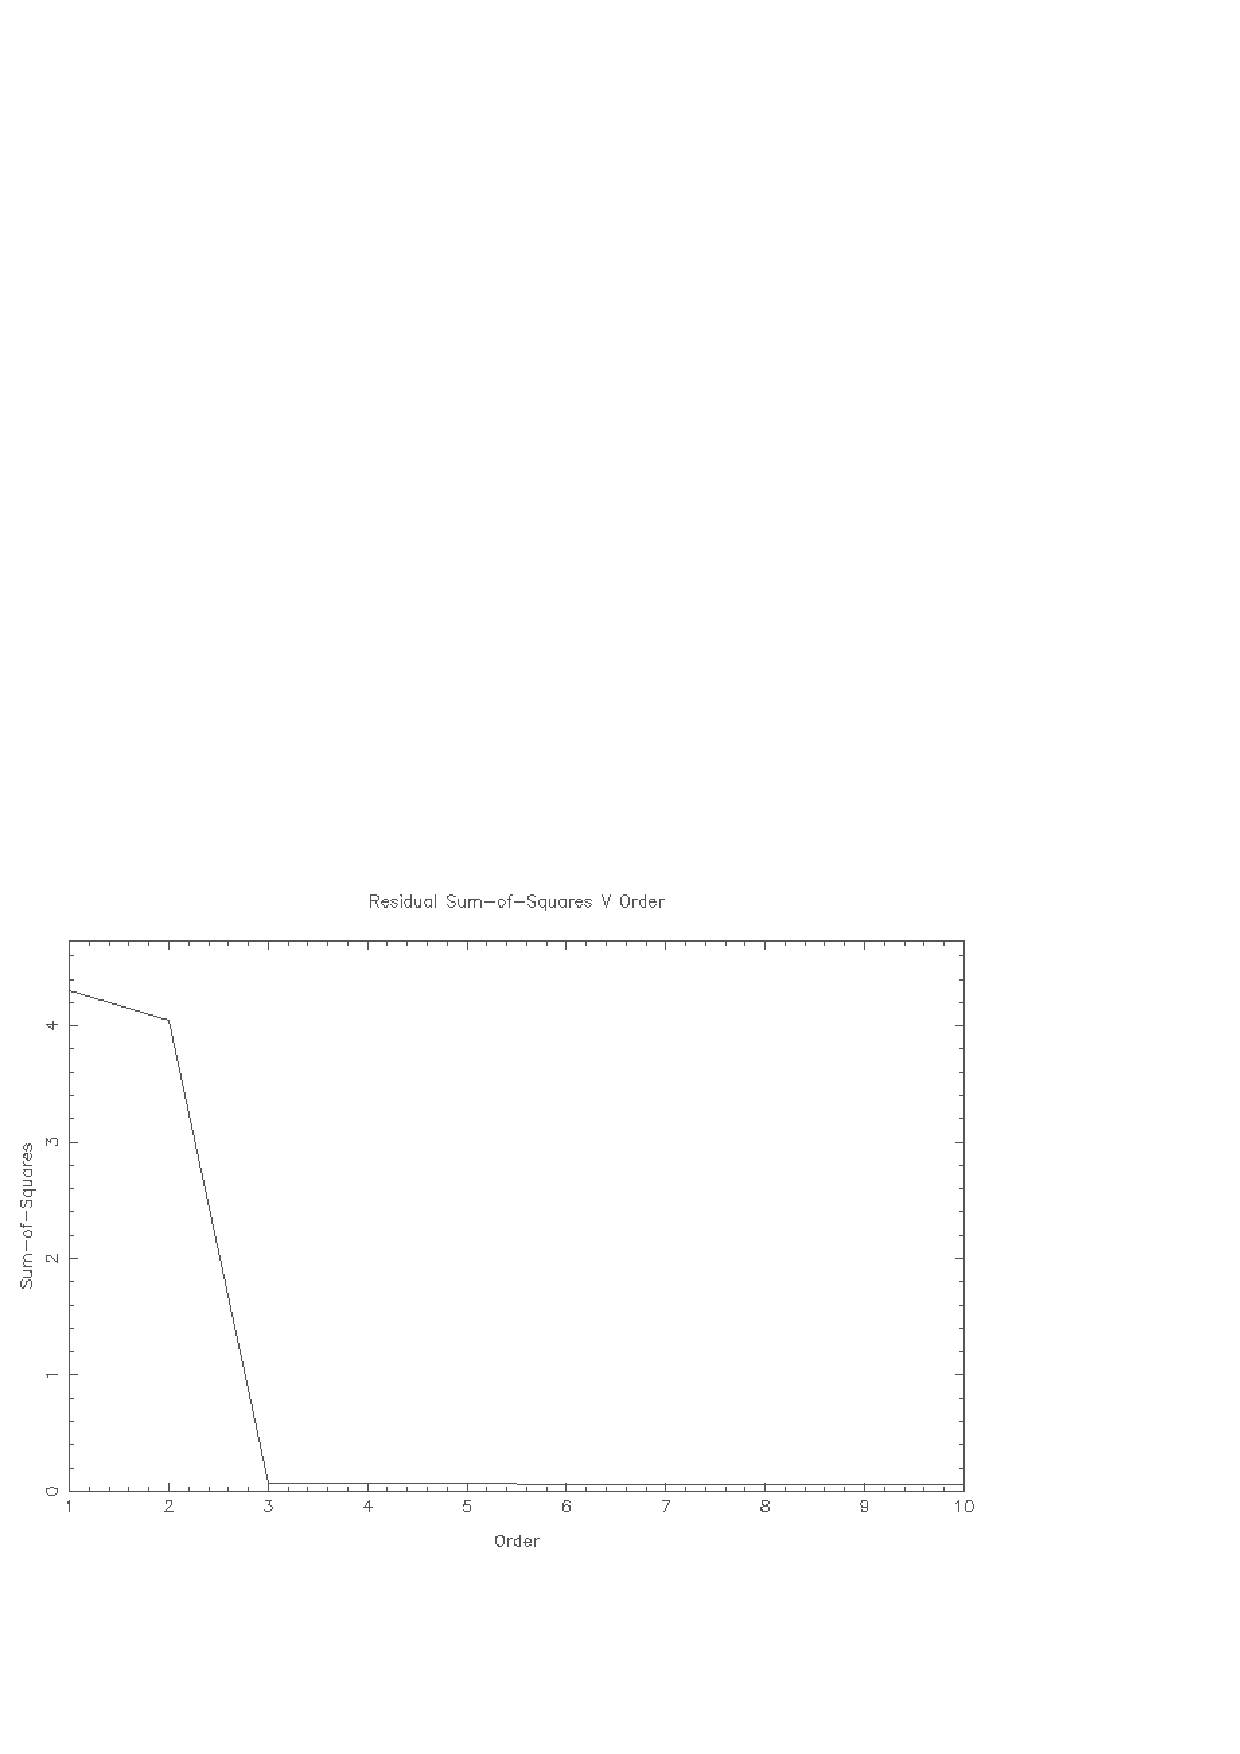
\includegraphics[height=105mm]{sc7_16}}
         {\leavevmode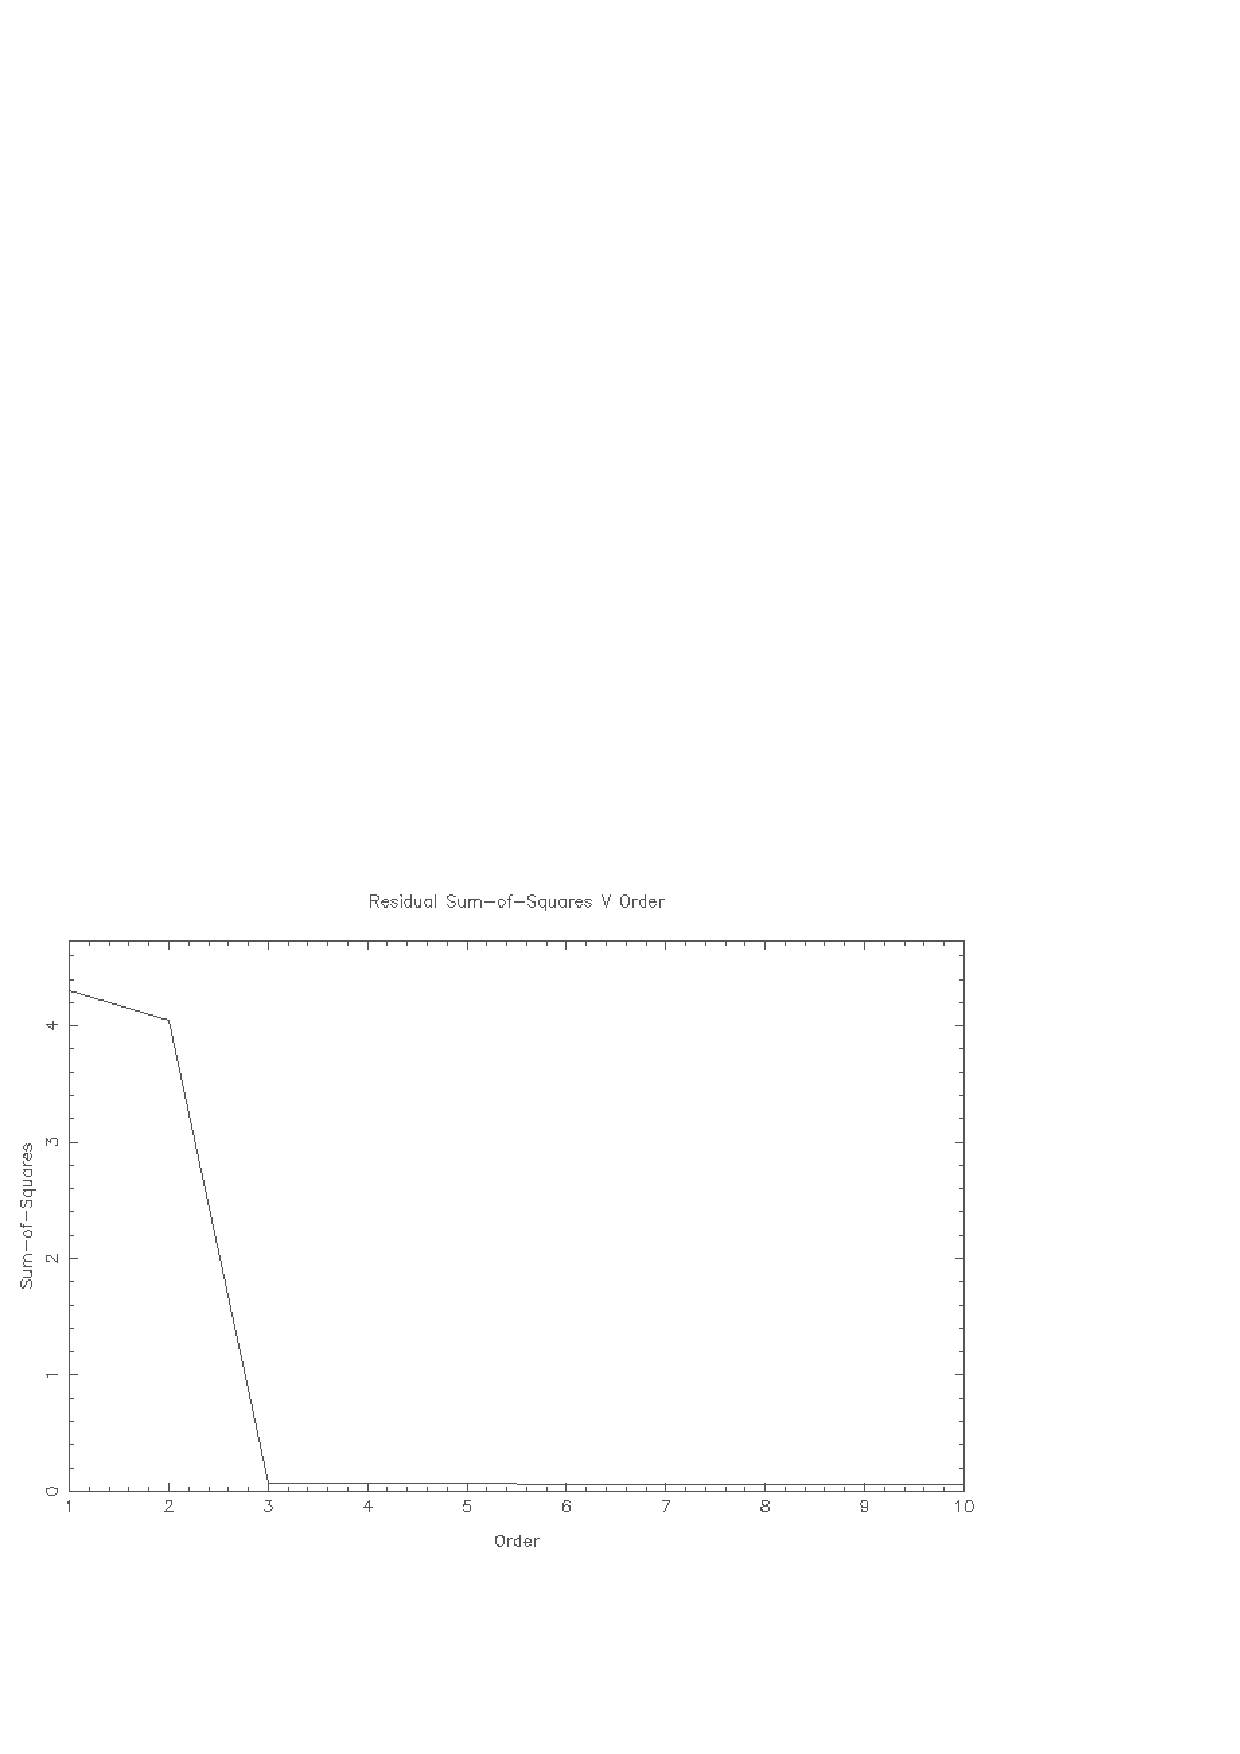
\includegraphics[height=136mm]{sc7_16}}

  \parbox{140mm}{
    \caption{The residuals with increasing order for a polynomial fit to
             the arc line curvature.}
    \label{poly_order}
  }
\end{center}
\end{figure}


If you reply {\tt yes} to the request to go on to next plot you will
be shown the residuals for a first order polynomial. Press return
again will show the second order fit and so on. Looking at the
residuals to the third order fit we can see they are less than
$\pm0.1$ pixels. At this display enter {\tt no} to the request to see
further orders.

The program then asks for the order you wish to use:
{\scspec{\small}{ }
\begin{verbatim}
ORDER - order for polynomial fitting /2/ >
\end{verbatim}
}

Enter {\tt 3} here and press return.

Now the data points and polynomial fit are displayed for the first arc
line (or tooth as it is described here). Again we can continue to look
at the data and fit for each of the arc lines.

When you reach the last line or type {\tt no} earlier you are asked if
you wish to produce a hard copy of the plots. For now select {\tt no}
and the program will ask if you want to accept the fitted polynomials:

{\scspec{\small}{ }
\begin{verbatim}
=========< C o n t i n u i t y   F i t s >=========

Accept : Accept fits
Retry  : Try again
Quit   : Give up

CHARACTER_VALUE - Continuity Fits /'ACCEPT'/ >
\end{verbatim}
}

Enter {\tt accept} to return to the main menu.

\subsection{Calibrating the wavelength axis}


With the straightening of the arc lines calculated the next step is to
calibrate the wavelength dispersion axis. From the main menu enter
{\tt disp} to select the 'Evaluate dispersion relation' option.

The dispersion screen is then shown on the xwindows display (see
\scspec{Figure~\ref{dispdisplay}, page~\pageref{dispdisplay},}{the
figure below}). The arc lines are listed with boxes to toggle the use
of that line in the calculations.

\begin{figure}
\begin{center}
  \scspec{\leavevmode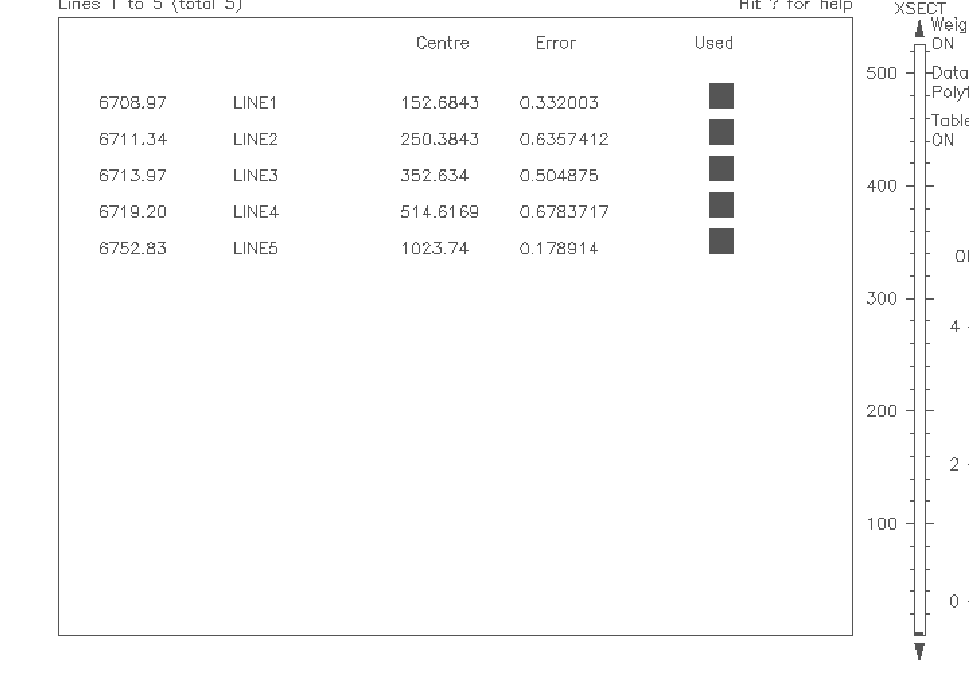
\includegraphics[height=105mm]{sc7_17}}
          {\leavevmode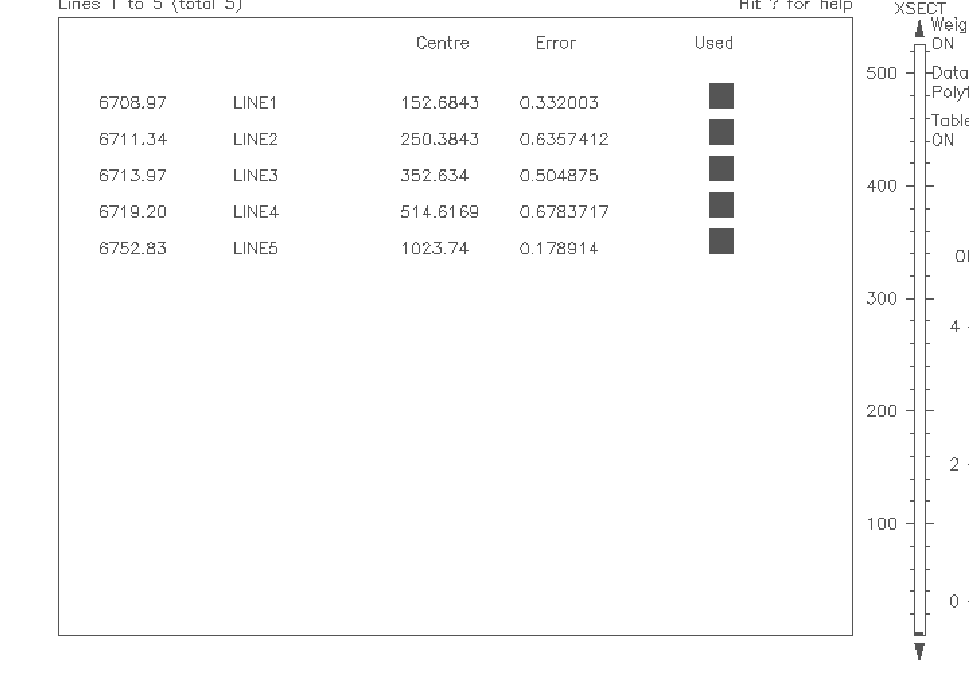
\includegraphics[height=136mm]{sc7_17}}

  \parbox{140mm}{
    \caption{The dispersion calibration control screen.}
    \label{dispdisplay}
  }
\end{center}
\end{figure}


On the far right of the display is a selector for the order of fit to be used
and then the y-axis (or X-section) number to perform the fit at.

In this case we shall use a 3rd order fit (which should already be
selected) and to perform the fit at a y-axis value of around 300. You
will need to click next to 300 in the slider at the right hand side of
the display. The marker should then be shown at 300.

Then carry out the fit, which solves the non-linear pixel value to
wavelength value relation, press {\tt f} while the cursor is in the
main panel.

The program then displays the polynomial used for the fit in the upper
panel and the residuals in the lower panel. Residuals of less than
$\pm0.05$ are usual for a good fit. See \scspec{Figure~\ref{dispfit},
page~\pageref{dispfit},}{the figure below} for an example fit.


\begin{figure}
\begin{center}
  \scspec{\leavevmode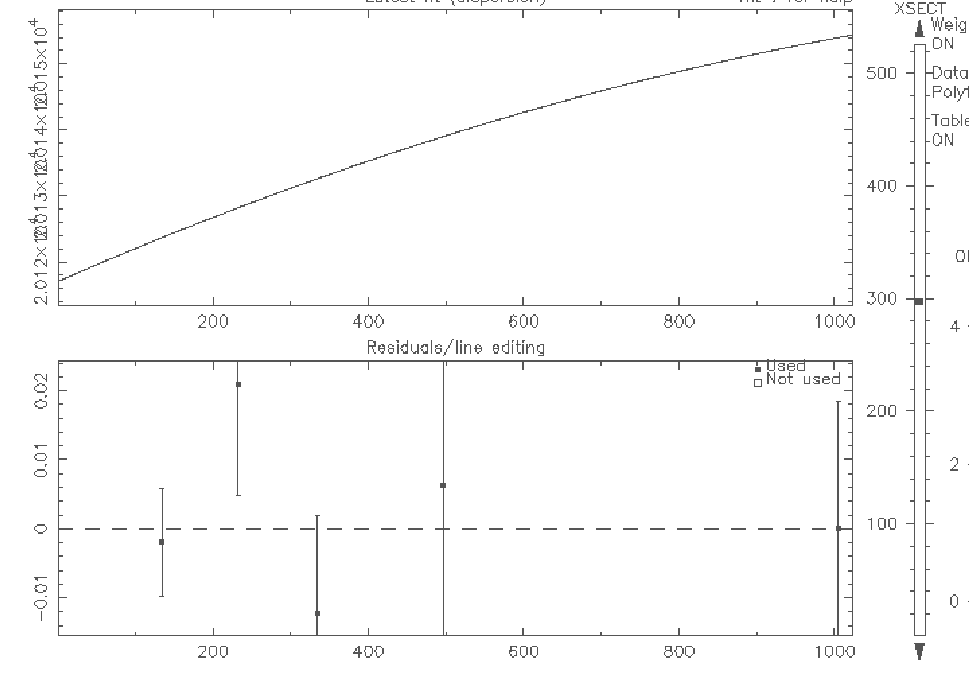
\includegraphics[height=105mm]{sc7_18}}
         {\leavevmode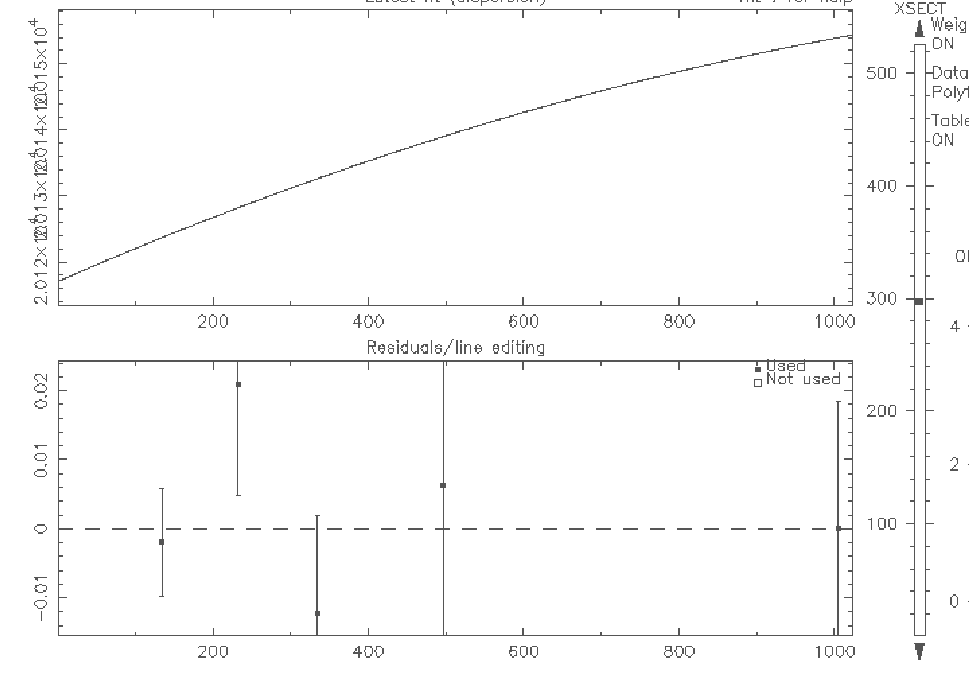
\includegraphics[height=136mm]{sc7_18}}

  \parbox{140mm}{
    \caption{An example dispersion fit, displaying the polynomial used
             for the fit in the upper panel and the residuals in the lower
             panel.}
    \label{dispfit}
  }
\end{center}
\end{figure}



We could then go on to try a 2nd order polynomial fit - select order
two by clicking the order selector at the right of the screen and
press {\tt f} again. You can see then residuals are now around
$\pm0.5$.

Select order 3 again and refit the data (press {\tt f} again).

When you are happy you press {\tt a} to accept the fit. Control now
reverts to the terminal window where you can opt to see tables of the
fit results. Enter {\tt no} to this and the next question regarding
copying fits from one line to another. You will be asked to confirm
the fits are ok.

When the fits are completed a line looking like:
{\scspec{\small}{ }
\begin{verbatim}
Minimum start wavelength = 6705.248, maximum end wavelength = 6754.836
\end{verbatim}
}

will have been displayed. These numbers are important and are used in
the scrunching step to come.

The program then returns to the main menu and reports the writing of
an .iar file which contains our polynomial fits.

We can now select exit to leave the program.

The .iar file generated is a simple ascii file and can be looked at with more:

{\scspec{\small}{ }
\begin{verbatim}
 % more arcframe2d.iar

 2d fit to data in image arcframe2d

image dimensions  1024 by   525
number of rows that could not be fitted =     0
maximum chi-squared error =       0.00
maximum degree polynomial used =   3
             1            0.3543959884354487D-07 -0.1650474022720115D-04
  0.2625885040194589D-01  0.6705221506967161D+04
             2            0.3544256762805665D-07 -0.1649068558149317D-04
  0.2625527448138038D-01  0.6705225714745435D+04
             3            0.3544542125840266D-07 -0.1647696602714036D-04
  0.2625177126897877D-01  0.6705229808939712D+04

....
\end{verbatim}
}

\subsection{Scrunching}

The .iar file can be used by the \xref{{\sc figaro}}{sun86}{}
\xref{{\bf iscrunch}}{sun86}{ISCRUNCH} program in order to correct
and calibrate your data files:

{\scspec{\small}{ }
\begin{verbatim}
 % iscrunch object2d
\end{verbatim}
}
You will then be asked for the name of the .iar file:
{\scspec{\small}{ }
\begin{verbatim}
FILE - (FIle) File containing results of 2D arc fit /''/ >
\end{verbatim}
}enter {\tt arcframe2d}.

The next question asks how many bins (pixels) you would like your new
image to have. The simplest answer is to keep the same number of
pixels that you had in your original image, hence for this file enter
{\tt 1024}

The next question ask if you want to sample your data in logarithmic
bins, enter {\tt false}.

You will now be asked for the start and end wavelengths of your data,
use the numbers noted earlier after the dispersion had been
calculated.
{
\scspec{\small}{ }
\begin{verbatim}
WSTART - (WStart) Wavelength of center of first bin /6693.583/ > 6705.248
WEND - (WEnd) Wavelength of center of last bin (or increment) /6759.628/ > 6754.836
\end{verbatim}
}

The next question asks if the data should be treated as a flux per
unit wavelength. Typically for data from spectrometers the answer to
this is {\tt false}.

Reply {\tt true} to use quadratic interpolation for the data at the next question.

The final question asks for the output filename, e.g. object2dscrunch:
{\scspec{\small}{ }
\begin{verbatim}
OUTPUT - (OUtput) Name of resulting scrunched image /''/ > object2dscrunch
\end{verbatim}
}

We can now view this scrunched file using:

{\scspec{\small}{ }
\begin{verbatim}
   % display object2dscrunch clear mode=pe accept
\end{verbatim}
}

which should look something like \scspec{Figure~\ref{scrunched},
page~\pageref{scrunched}.}{the figure below.}

\begin{figure}
\begin{center}
  \scspec{\leavevmode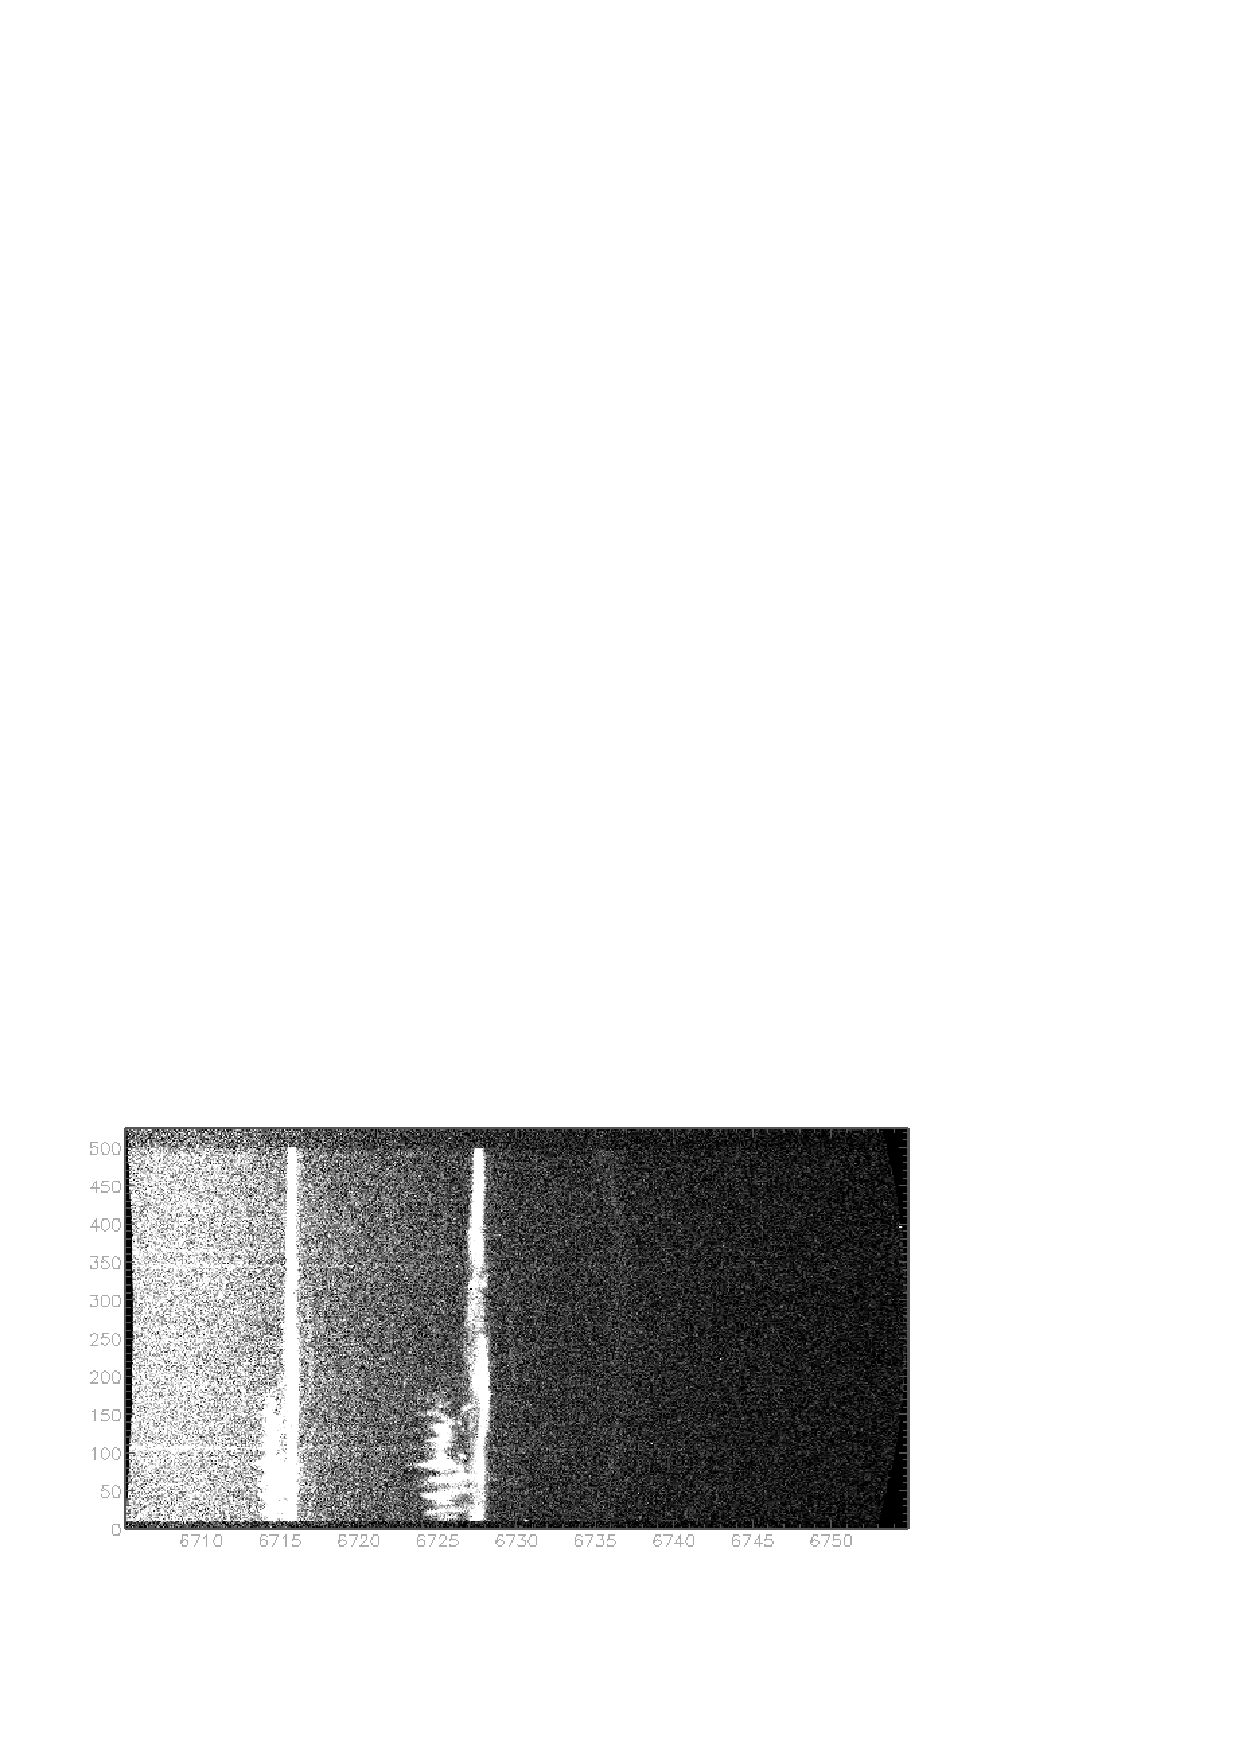
\includegraphics[height=105mm]{sc7_19}}
         {\leavevmode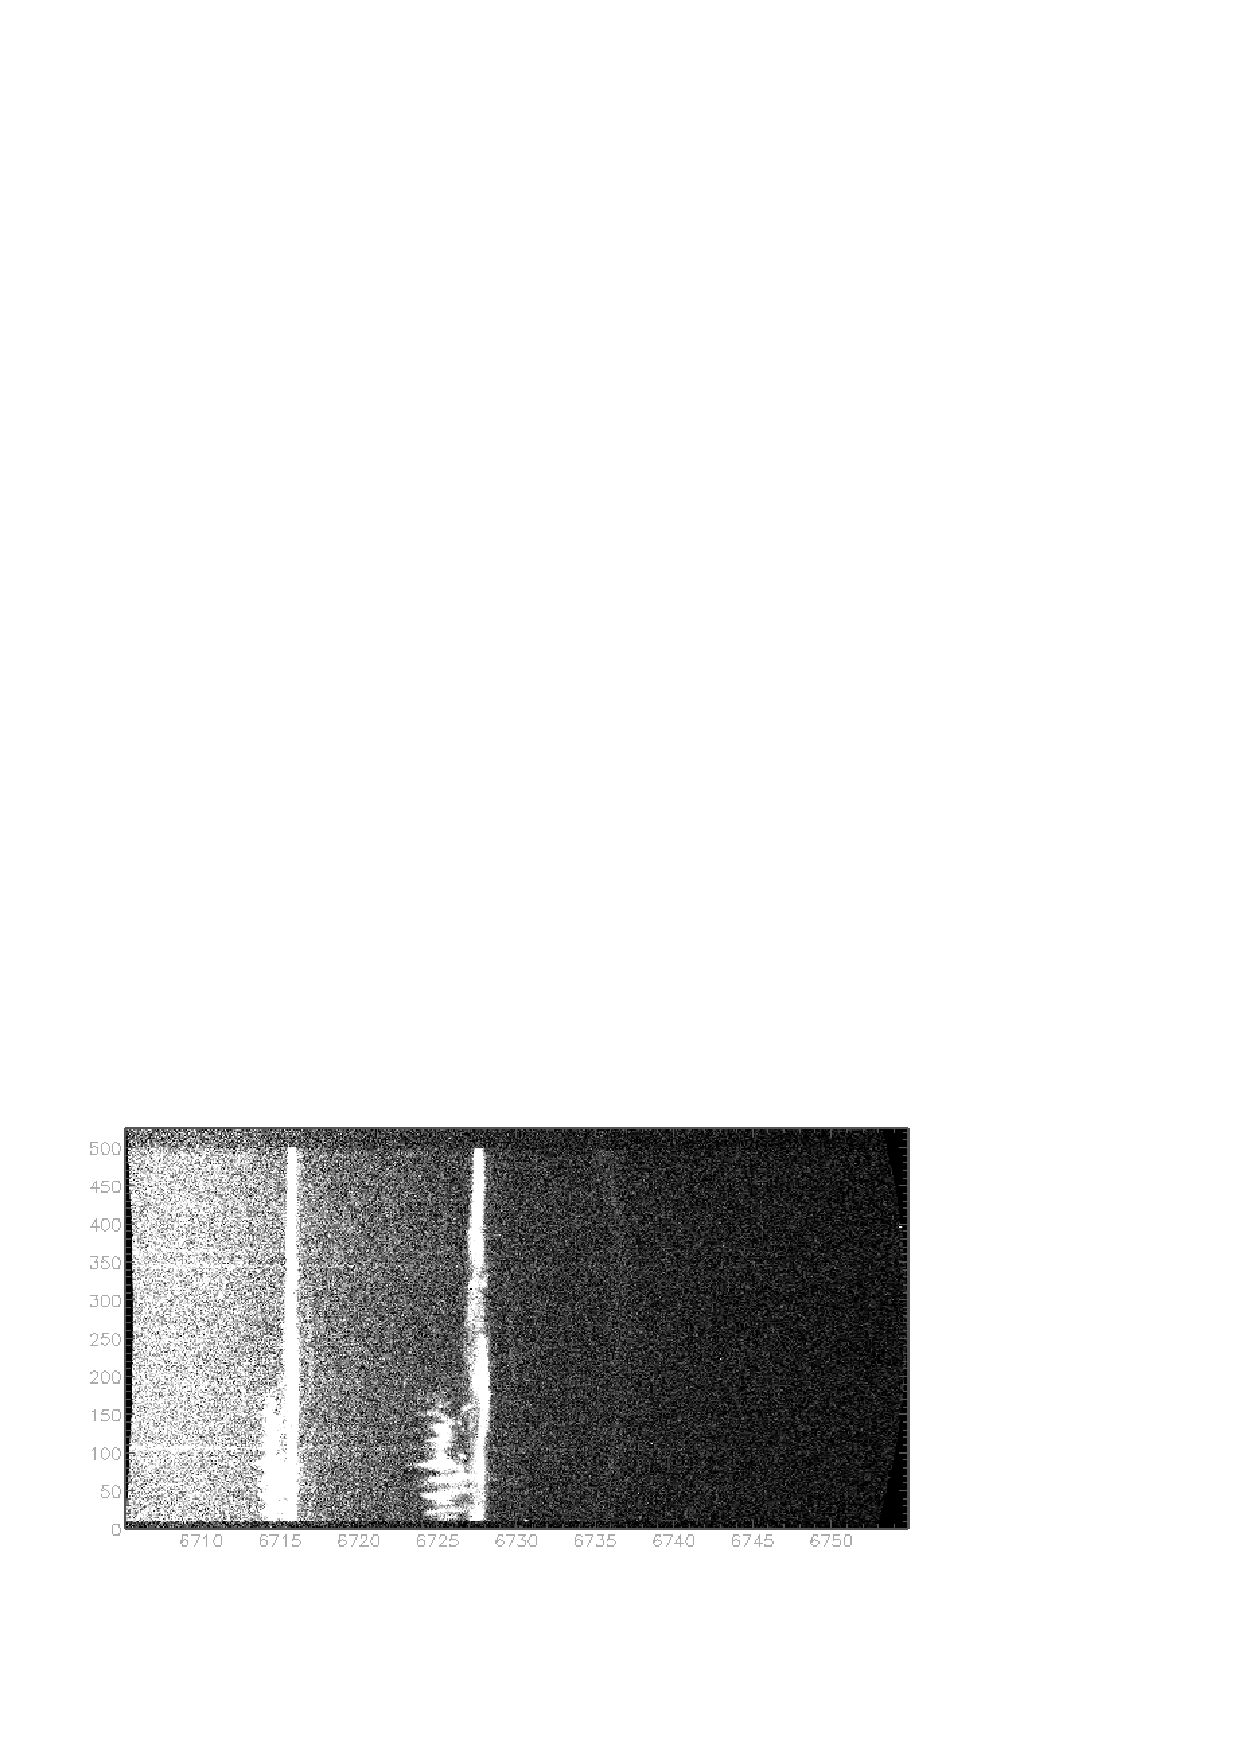
\includegraphics[height=136mm]{sc7_19}}

  \parbox{140mm}{
    \caption{The data frame, now calibrated and curvature corrected.}
    \label{scrunched}
  }
\end{center}
\end{figure}


A further check on the process is to scrunch the arc frame, in order
to check that the arc lines do indeed come out perfectly straight.


\subsection{Blaze correction}

To remove the wavelength dependent sensitivity or blaze from the data
we need to use a quartz flat. The file quartz2dscrunch.sdf is a ready
scrunched quartz lamp image.

{\scspec{\small}{ }
\begin{verbatim}
   % display object2dscrunch mode=pe accept
   % lutgrey
\end{verbatim}
}

The bright line towards the right of the image is a ghost. We wish to
generate a smooth fit to the quartz lamp and the easiest way of doing
this is to add together the rows to form a single spectrum. We use the
values for the range in y-axis obtained earlier from measuring the arc
lines.

{\scspec{\small}{ }
\begin{verbatim}
   % extract quartz2dscrunch 13 493 quartzspec
\end{verbatim}
}

This generates a spectrum quartzspec.sdf which we can view with

{\scspec{\small}{ }
\begin{verbatim}
   % splot quartzspec whole=true autoscale=true hardcopy=false label=quartz
\end{verbatim}
}

\begin{figure}
\begin{center}
  \scspec{\leavevmode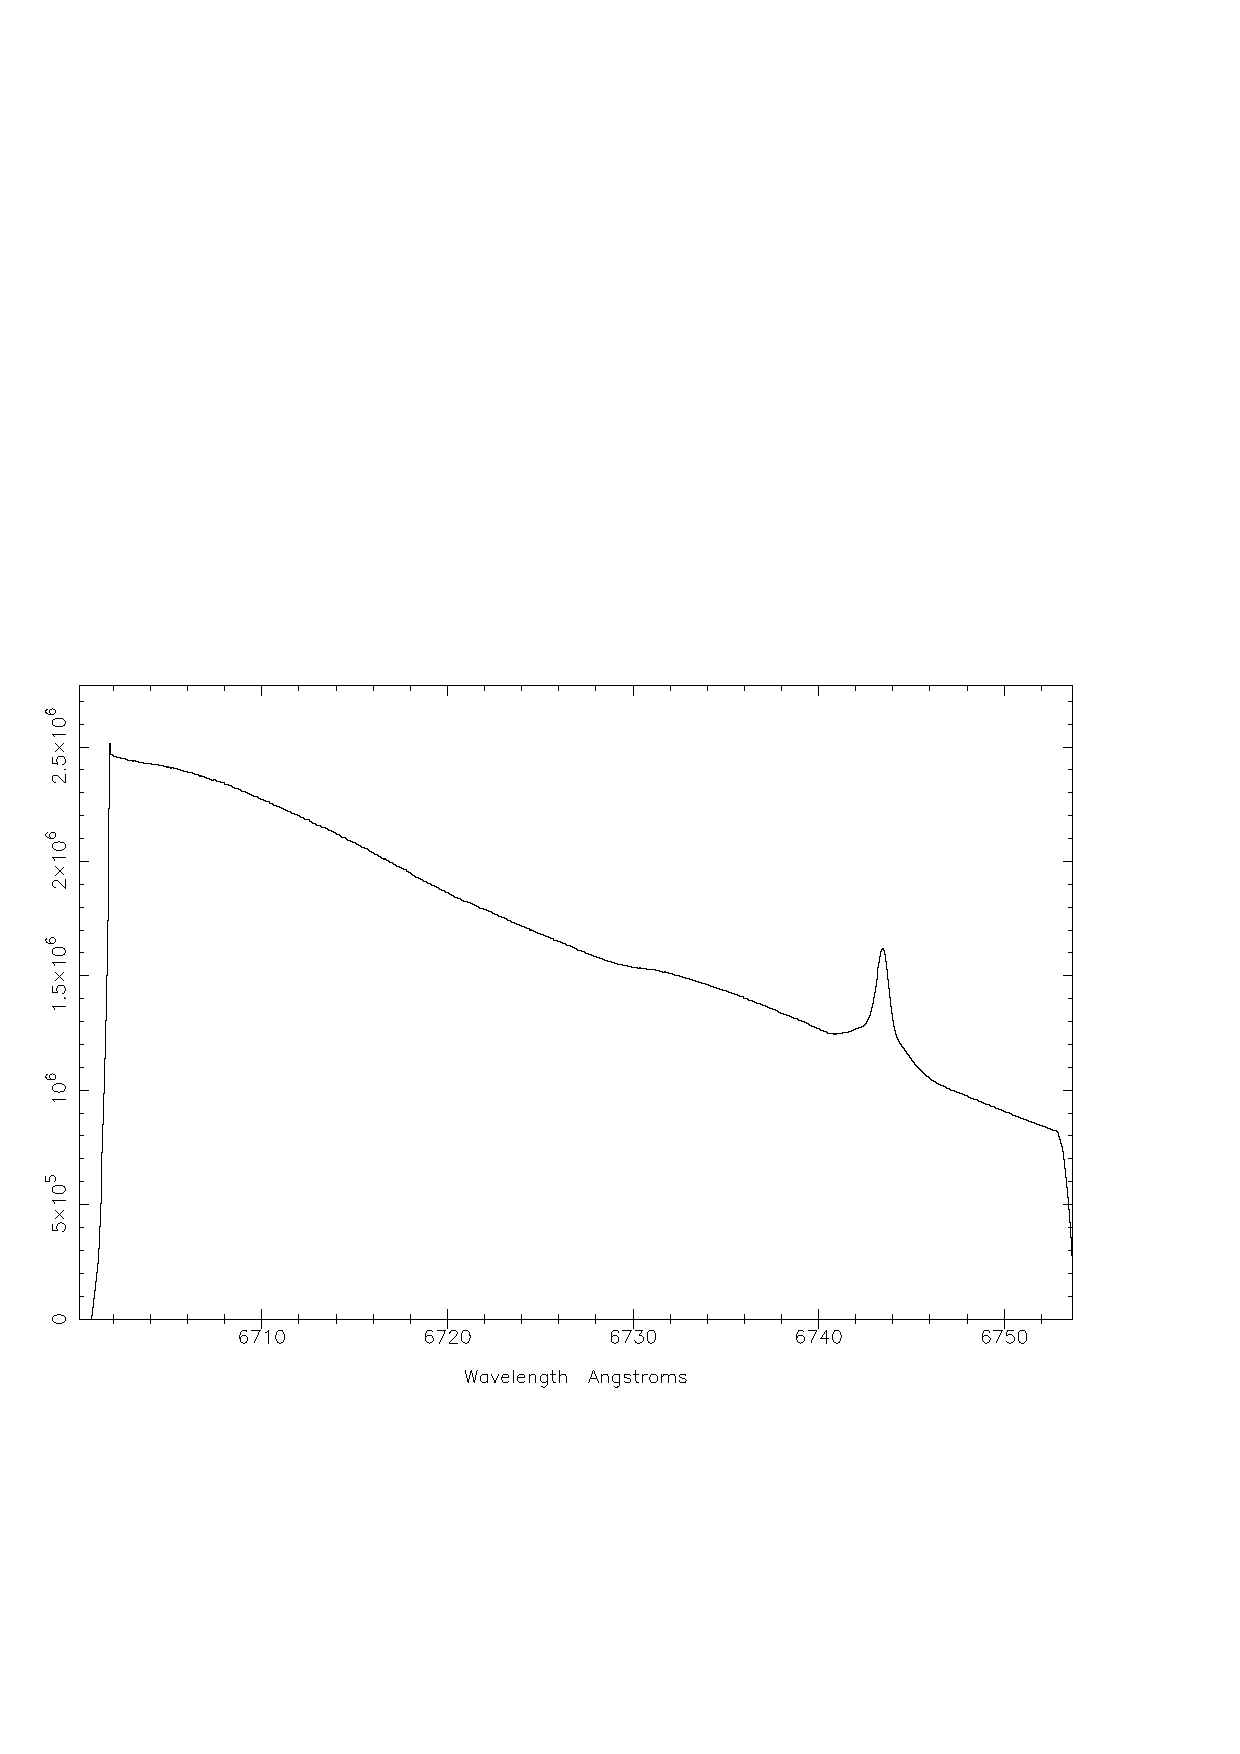
\includegraphics[height=105mm]{sc7_20}}
          {\leavevmode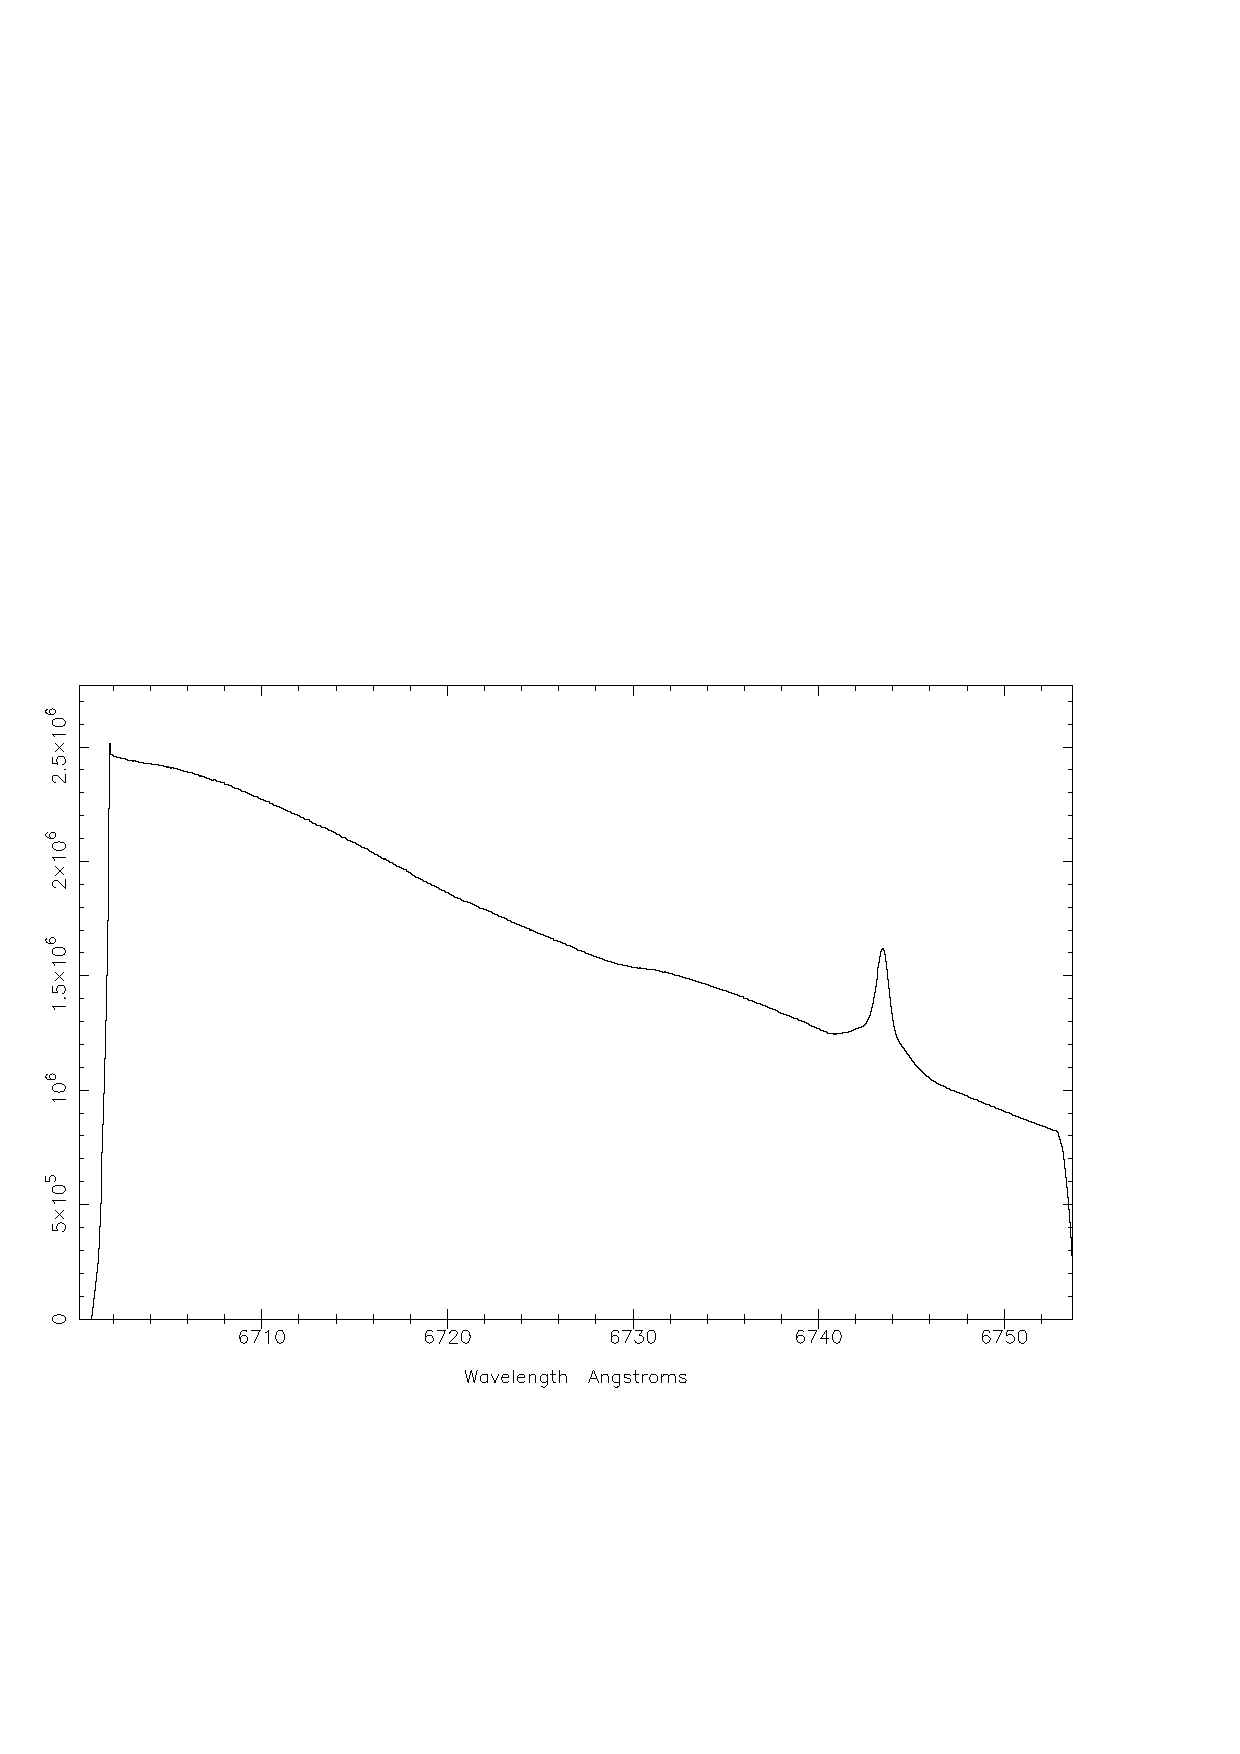
\includegraphics[height=136mm]{sc7_20}}

  \parbox{140mm}{
    \caption{The extracted quartz spectrum.}
    \label{quartzfit}
  }
\end{center}
\end{figure}

As can be seen in \scspec{Figure~\ref{quartzfit},
page~\pageref{quartzfit},}{the figure below,} this spectrum has zero
values at each end and the ghost line appears superimposed on the
quartz lamp continuum. In order to remove these effects and obtain
just the continuum we fit a polynomial curve to the data. We use the
\xref{{\sc figaro}}{sun86}{} \xref{{\bf cfit}}{sun86}{CFIT} command:

{\scspec{\small}{ }
\begin{verbatim}
   % cfit output=quartzfit
\end{verbatim}
}

Use the cursor and mark points (using the {\tt a} key) along the
spectrum, including points at the start and end where we have no data
and ignoring the ghost line. When you have finished this press {\tt x}
the exit. The fitted line is then drawn over the spectrum.



We can view this on its own with

{\scspec{\small}{ }
\begin{verbatim}
   % splot quartzfit whole=true autoscale=true hardcopy=false label=quartzfit
\end{verbatim}
}

We now have a smooth spectrum to divide into our data but before we do
this one further stage is to normalize this curve. To do this we need
to find the mean value for the quartzfit spectrum:

{\scspec{\small}{ }
\begin{verbatim}
   % stats quartzfit
\end{verbatim}
}

For my fitted spectrum this gave these results:

{\scspec{\small}{ }
\begin{verbatim}
   Pixel statistics for the NDF structure
/home/mips/star/starlink/cookbook/example/quartzfit

      Title                     : QUARTZ SII FOR HONEYCOMB
      NDF array analysed        : DATA

         Pixel sum              : 1.7037235E9
         Pixel mean             : 1663793
         Standard deviation     : 511041.5
         Minimum pixel value    : 794998.6
            At pixel            : (1024)
            Co-ordinate         : (6753.693)
         Maximum pixel value    : 2492099
            At pixel            : (1)
            Co-ordinate         : (6700.157)
         Total number of pixels : 1024
         Number of pixels used  : 1024
\end{verbatim}
}

The key number is the pixel mean value of 1663793, which we will
divide the spectrum with to give a mean value of 1.

{\scspec{\small}{ }
\begin{verbatim}
   % icdiv quartzfit 1663793 quartzfitnorm
\end{verbatim}
}

We can now finally use this normalised spectrum to correct our
observed data using the \xref{{\sc figaro}}{sun86}{}
\xref{{\bf isxdiv}}{sun86}{ISXDIV} command:

{\scspec{\small}{ }
\begin{verbatim}
   % isxdiv object2dscrunch quartzfitnorm object2dscrunchnorm
\end{verbatim}
}

This command divides the quartz spectrum into each row of our data
frame to produce the quartz corrected file {\tt
object2dscrunchnorm.sdf} (see \scspec{Figure~\ref{finalcal},
page~\pageref{finalcal}.}{the figure below.}

\begin{figure}
\begin{center}
  \scspec{\leavevmode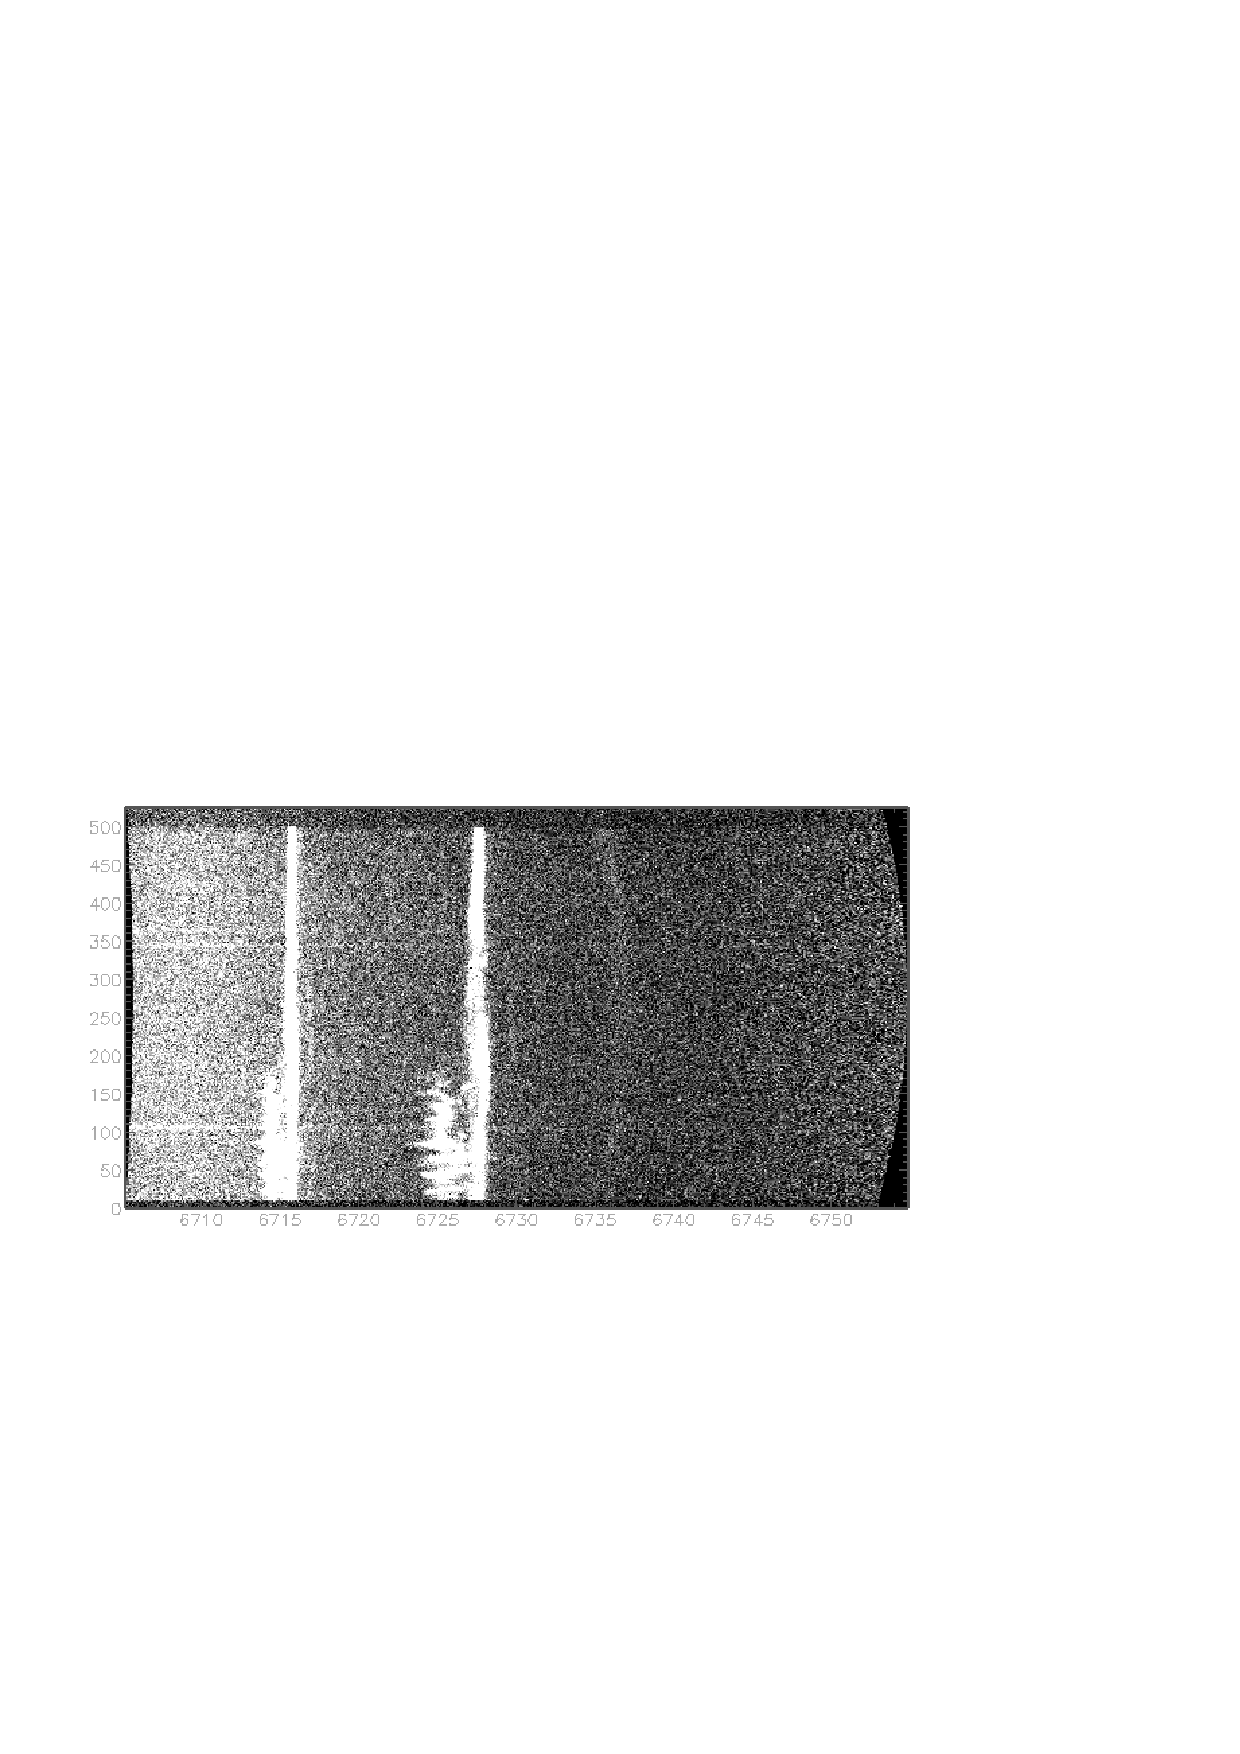
\includegraphics[height=105mm]{sc7_21}}
          {\leavevmode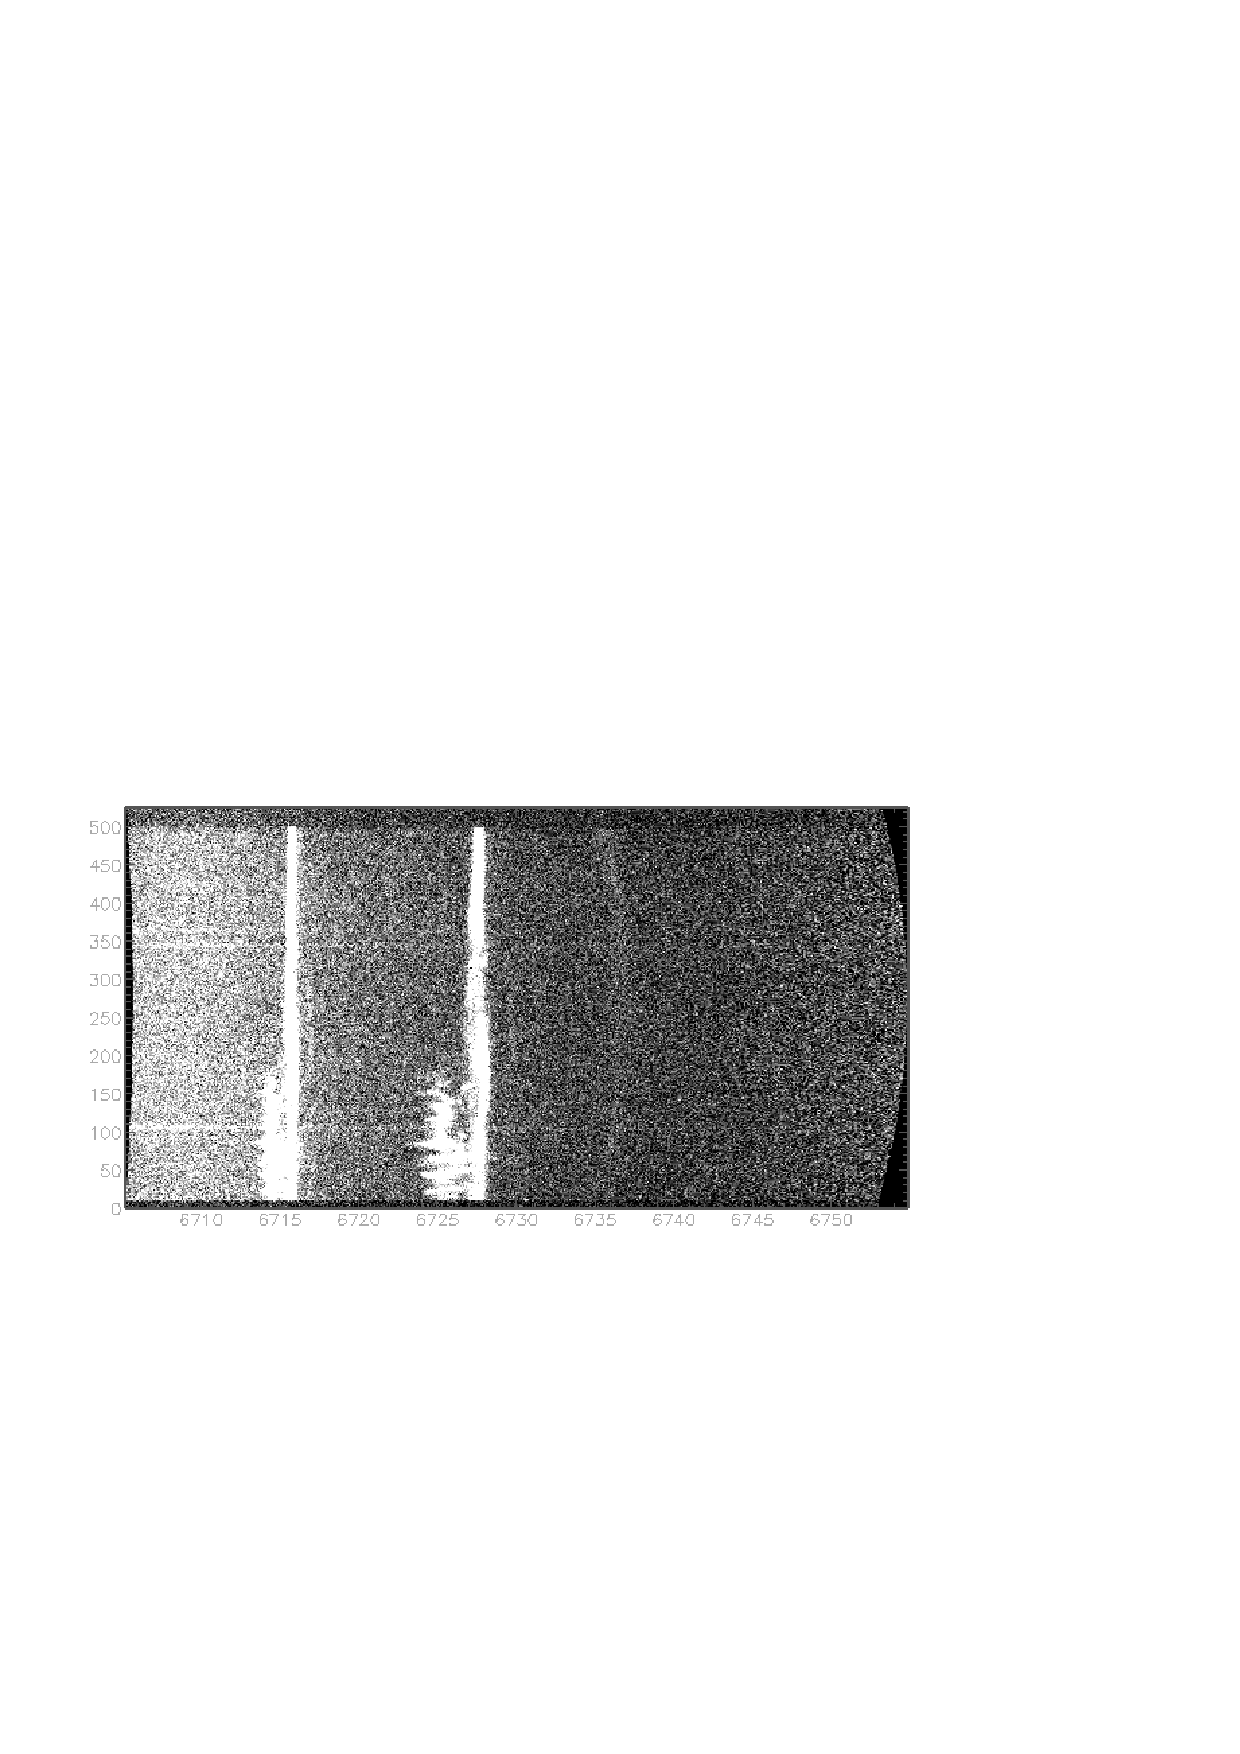
\includegraphics[height=136mm]{sc7_21}}

  \parbox{140mm}{
    \caption{The calibrated data frame, corrected for the instrumental
             response.}
    \label{finalcal}
  }
\end{center}
\end{figure}
 ) with:

{
\scspec{\small}{ }
\begin{verbatim}
   % display object2dscrunchnorm clear mode=sc low=6 high=25 accept
   % lutgrey
\end{verbatim}
}


With the data calibrated you have now completed the data reduction of
a 2-D longslit spectral array. For analysis of this data you may want
to use the \xref{{\sc twodspec}}{sun16}{}\cite{twodspec} {\sc
longslit} package or \xref{{\sc dipso}}{sun50}{}\cite{dipso}.


%%%%%%%%%%%%%%%%%%%%%%%%%%%%%%%%%%%%%%%%%%%%%%%%%%%%%%%%%%%%%%%%%%%%%%%%%%%
\section{\mlabel{cookies}Cookies}
\markboth{Cookies}{\stardocname}

\subsection{\mlabel{cook_parameter_editor}How to Use the {\bf echmenu}
            Parameter Editor}

In the \htmlref{worked example}{simple_worked_example}
\xref{{\bf echmenu}}{sun152}{ECHMENU} was extensively used.
\xref{{\sc echomop}}{sun152}{} is very flexible; there are a large number of
parameters available which can be tuned to suit your data.  Parameter
values can be supplied on the command line, for example:

{
\scspec{\small}{ }
\begin{verbatim}
   % echmenu tune_mxskypix=31
\end{verbatim}
}

This is useful as normally \xref{{\tt
tune\_mxskypix}}{sun152}{par_TUNE_MXSKYPIX} will simply take its default
value (21) without ever prompting.

Another method for checking and setting parameter values is to use the
parameter editor built in to {\bf echmenu}\@.  If, for example, you want
to inspect the parameters for
\xref{Option~4 {\sl Determine dekker/object extent}}{sun152}{option4},
you type \verb+-4+ at the main {\bf echmenu} prompt:

{
\scspec{\small}{ }
\begin{verbatim}
    - Option number /'or Y for default=1'/ > -4
\end{verbatim}
}

A display like this will appear:

{
\scspec{\small}{ }
\begin{verbatim}
    Parameters for: Determine dekker/object extent. (ECH_SPATIAL)
    A * means the parameter must be set; the displayed value is the default.
    Select number of parameter to change:

     0. Exit
     1. INPTIM          =*''            9. TUNE_MAXPOLY    = 50
     2. PFL_INTERACT    =*TRUE         10. TUNE_MXSKYPIX   = 21
     3. PFL_MODE        =*'A'          11. TUNE_OBJABV     = 0
     4. SLITIM          =*''           12. TUNE_OBJBLW     = 0
     5. TUNE_DIAGNOSE   = FALSE        13. TUNE_PFLSSAMP   = 301
     6. TUNE_DEKABV     = 0            14. TUNE_SKYHILIM   = 0.5
     7. TUNE_DEKBLW     = 0            15. TUNE_USE_NXF    = 0.2
     8. TUNE_DEKTHR     = 0.8

    - Parameter number /1/ >
\end{verbatim}
}

You can see that each of the task parameters is displayed with the current
value, except for parameters marked with a \verb+*+, for which the default
is shown.  To change a parameter you type its number ({\it{e.g.}} \verb+10+
for \verb+tune_mxskypix+) and then enter the new value at the prompt.

When you are happy with the values set, enter \verb+0+ (zero) to exit the
parameter editor.


\subsection{\mlabel{cook_airmass}Looking at FITS Header Cards: Air Mass}

There are several tools available for looking at FITS headers in
\xref{{\sc{kappa}}}{sun95}{}.
The simplest is \xref{{\tt fitslist}}{sun95}{FITSLIST} which displays
the complete list of FITS header cards.  For example,

{
\scspec{\small}{ }
\begin{verbatim}
   % kappa    # Only needed once per session.
   ... setup messages ...
   % fitslist object
\end{verbatim}
}

will display the FITS header for the example dataset included with this
document.  This can be used to retrieve information such as the air mass:

{
\scspec{\small}{ }
\begin{verbatim}
   % fitslist object | grep -i air
   AMEND   =             1.350784 / Airmass at approx. end of exposure
   AIRMASS =             1.323036 / Airmass at approx. start of exposure
   AMSTART =             1.323036 / Airmass at approx. start of exposure
\end{verbatim}
}

As you can see, the above example has retrieved three cards matching the
string \verb+air+, the \verb+-i+ option for {\bf grep} ensures that the
search is not case-sensitive.

Having extracted these data from the FITS header, we can now estimate
the air mass for the exposure\scspec{---}{ - }about 1.337 in the example
(that's the mean of the start and end air masses).


\subsection{\mlabel{cook_wavelength}Looking at FITS Header Cards:
            Wavelength Coverage}

Another use for \xref{{\tt fitslist}}{sun95}{FITSLIST} might be to
track down details of the wavelength range covered by the spectrum.
Four invocations of {\bf fitslist} will get all the information needed:

{
\scspec{\small}{ }
\begin{verbatim}
   % kappa    # Only needed once per session.
   ... setup messages ...
   % fitslist object | grep -i wavelength
   CENWAVE =                 4499 /Approx. central wavelength (Angstroms)
   % fitslist object | grep -i dispersion
   DISPERSI=                   33 / Nomimal dispersion (Angstroms/mm)
   % fitslist object | grep -i pixel
   CCDXPIXE=            24.000000 / Size of unbinned pixels in x (micron)
   CCDYPIXE=            24.000000 / Size of unbinned pixels in y (micron)
   % fitslist object | grep -i ccd.size
   CCDXSIZE=                 1124 / X dimension of digitised CCD frame
   CCDYSIZE=                 1124 / Y dimension of digitised CCD frame
\end{verbatim}
}

In this example, we can ignore the \verb+CCDY+ cards as these refer
to the cross-dispersion direction of the image of the spectrum (I'm
assuming that this is the example dataset \verb+object+ again here).
If you have rotated your data frames then the \verb+CCDY+ cards
should be used instead.

Using this simple formula we can determine
the approximate wavelength range covered:

\begin{htmlonly}
\begin{verbatim}
   wavelength_range = CCDXSIZE x CCDXPIXE x DISPERSI
\end{verbatim}
\end{htmlonly}
\begin{latexonly}
\begin{displaymath}
\lambda\lambda = {\tt{CCDXSIZE}} \times {\tt{CCDXPIXE}} \times {\tt{DISPERSI}}
\end{displaymath}
\end{latexonly}

Appropriate units should be used, for the example above this comes to
a coverage of about 890\AA , centred at 4499\AA\@.  This information can
be useful when trying to identify lines in an arc spectrum, and for
constraining the automatic arc-line identifier in
\xref{{\bf echmenu}}{sun152}{option10}\@.

If the information you need is not present in the FITS
headers you will have to consult the observatory's instrument manual.


\subsection{\mlabel{cook_ccdchar}Looking at FITS Header Cards: CCD
            Characteristics}

Another common use for \xref{{\bf fitslist}}{sun95}{FITSLIST} is to
get the details of the \htmlref{CCD}{gl_ccd}
\htmlref{output transfer characteristic}{gl_gain}
and \htmlref{readout noise}{gl_readout_noise}\@.
Two invocations of {\bf fitslist} will get all the information needed:

{
\scspec{\small}{ }
\begin{verbatim}
   % kappa    # Only needed once per session.
   ... setup messages ...
   % fitslist object | grep -i noise
   READNOIS=             5.300000 / Readout noise (electrons)
   % fitslist object | grep -i -e gain -e adu
   GAIN    =             1.300000 / Electrons/ADU conversion factor
\end{verbatim}
}

The second {\bf grep} searches for both `gain' and `adu' at the same
time\scspec{---}{ - }it so happens that both are present in the record
we are after.

If the information you need is not present in the FITS
headers you will have to consult the observatory's CCD manual.

\subsection{\mlabel{cook_finding_the_spectrum}Problems Finding the Spectrum}

The first thing to check if you can't see the spectrum clearly when
running \xref{{\bf echmenu}}{sun152}{ECHMENU}
\xref{Option~1}{sun152}{option1}, as in
\scspec{Figure~\ref{fi_order_locate} (see page~\pageref{fi_order_locate})}
{the figure below,} is that the
image is correctly oriented with the spectrum dispersed from left-to-right.

\begin{htmlonly}
\begin{figure}
\begin{center}
  \leavevmode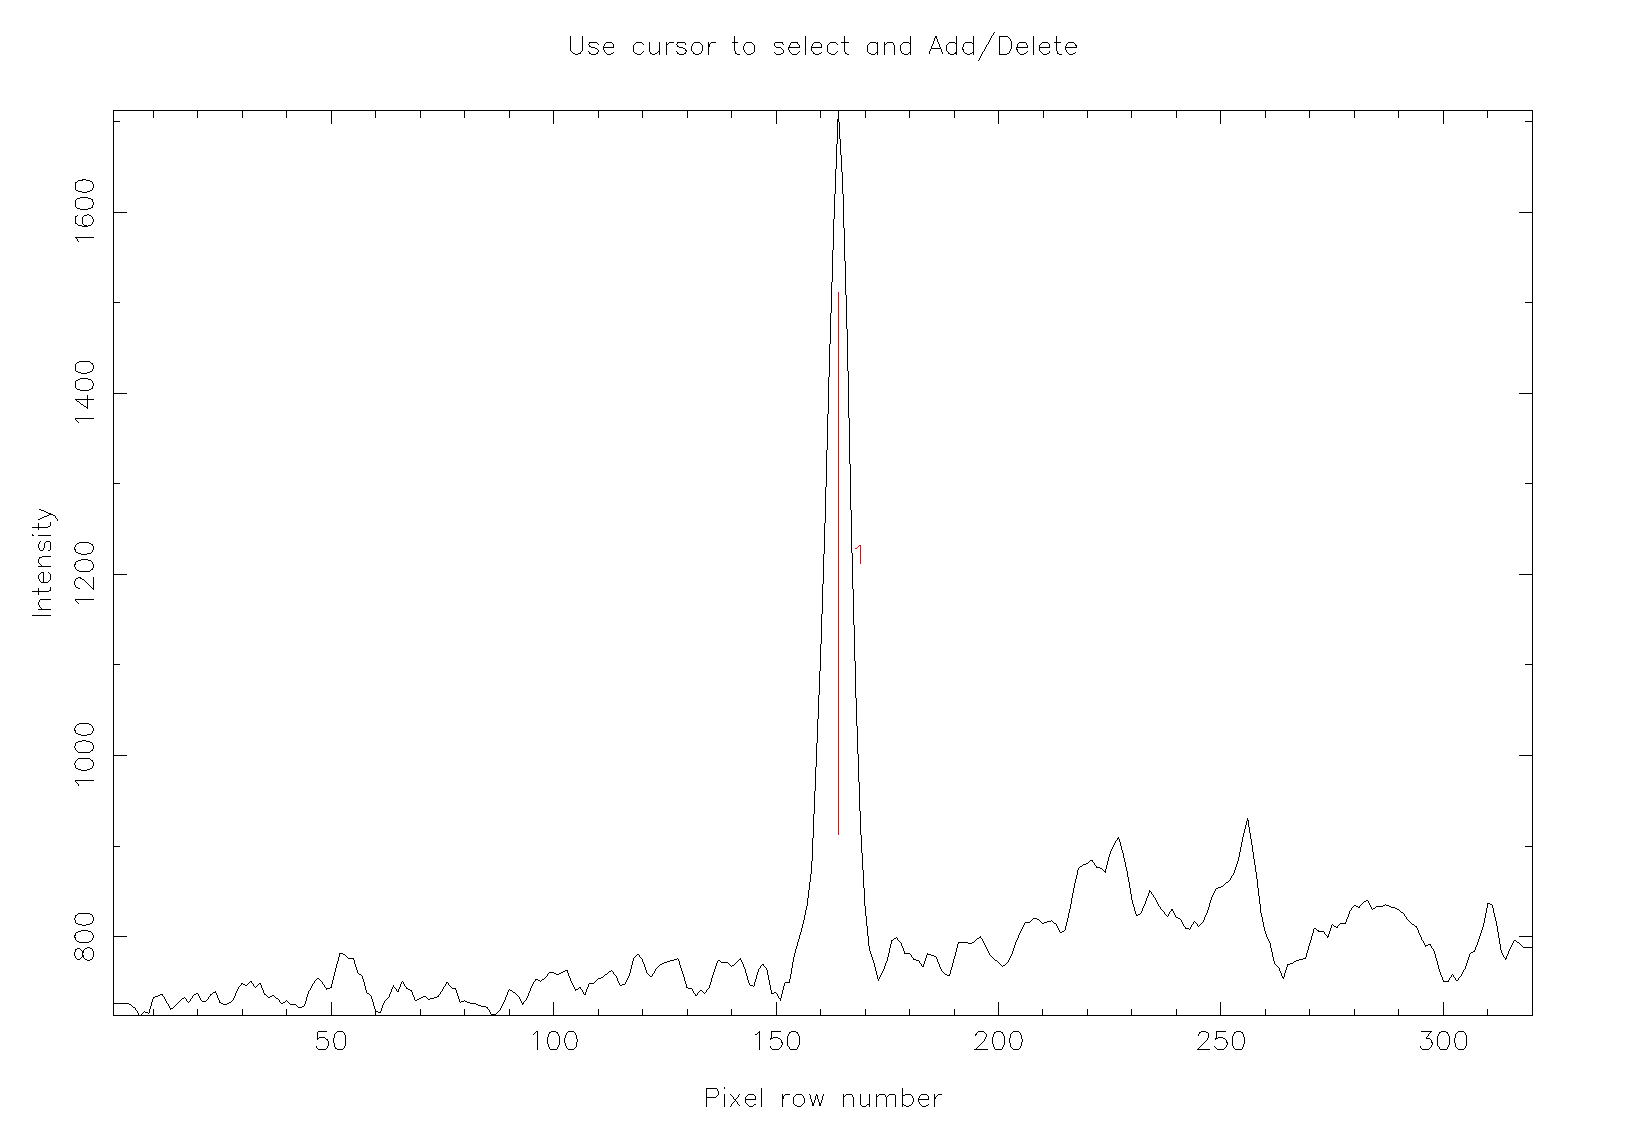
\includegraphics[height=136mm]{sc7_10}

  \parbox{140mm}{
    \caption{Order location: a cross-dispersion section produced using
             {\bf echmenu} Option~1 {\sl Start a reduction.}}
    \label{fi_order_locate_again}
  }
\end{center}
\end{figure}
\end{htmlonly}

See \scspec{\S\ref{inspecting_the_images}}
{\htmlref{Inspecting the Images}{inspecting_the_images}} for details of how
to check the orientation.  Perhaps the `zeroth' thing to check is that you
have chosen the correct image for the parameter
\xref{{\tt{tracim}}}{sun152}{par_TRACIM}\@.

If you find that {\bf echmenu} Option~1 does not automatically find the
spectrum, and you can't see it in the displayed plot, the next thing to
try is a simple plot of a sum of all the columns of the image.  This can
be done with a series of \xref{{\sc figaro}}{sun86}{} commands:

{
\scspec{\small}{ }
\begin{verbatim}
   % figaro   # Only needed once per session.
   ... setup messages ...
   % ystract object min max slice
   % splot slice soft=xw accept
\end{verbatim}
}

You should see the spectrum somewhere in this section plot.  Inspect the
X-axis and redisplay the section, but this time zoom-in on the spectrum
(in the example data the spectrum is at about Y=183).

{
\scspec{\small}{ }
\begin{verbatim}
   % splot slice xstart=170 xend=200 soft=xw whole=f accept
\end{verbatim}
}

It should now be possible to decide where the centre of the spectrum is
by eye, or using the {\sc figaro} command \xref{{\bf icur}}{sun86}{ICUR}
to measure the display.

Once you have decided where the spectrum is, you can write this into the
{\sc echomop}
\xref{reduction structure file}{sun152}{reduction_file} using {\sc figaro}
\xref{{\bf creobj}}{sun86}{CREOBJ} and
\xref{{\bf setobj}}{sun86}{SETOBJ}:

{
\scspec{\small}{ }
\begin{verbatim}
   % creobj _integer 1 rdf1.more.echelle.order_ypos
   % setobj 183 'rdf1.more.echelle.order_ypos(1)'
   % setobj 1 rdf1.more.echelle.no_of_orders
\end{verbatim}
}

This above assumes the reduction structure file is called \verb+rdf1+\@.
Notice that you have to mark the fact that one `order' ({\it{i.e.}} spectrum)
has been found.  Once you have added this information you can proceed to
try \xref{{\bf echmenu} Option~2}{sun152}{option2}\@.


\subsection{\mlabel{cook_tracing}Tracing Strategies}

Usually the default value {\tt C}, `centroid' for
\xref{{\tt trace\_mode}}{sun152}{par_TRACE_MODE} works reasonably
well. Running \xref{{\bf echmenu}}{sun152}{ECHMENU} \xref{Option~3
{\sl Clip fitted traces}}{sun152}{option3}, and performing some small
interactive adjustments, results in a good, clean spectrum trace.
Sometimes, however, the object spectrum cannot be used for
tracing\scspec{---}{ - }there may be significant absorption features
present, the object frame may be severely contaminated with cosmic-ray
defects.

If a flat-field frame is available this can sometimes be used for tracing.
Such a frame must have been exposed with the \htmlref{dekker}{gl_dekker}
not completely open;
we need to be able to find the edges of the dekker on the frame.
To trace a flat field, proceed in the normal way, but set \xref{{\tt
trace\_mode=e}}{sun152}{par_TRACE_MODE} which stands for `edges':

{
\scspec{\small}{ }
\begin{verbatim}
   TRACE_MODE - Type of order tracing to use /'C'/ > E
\end{verbatim}
}

The trace will then be determined as the point mid-way between the
edges of the dekker.

Another alternative to tracing the target object spectrum is to trace the
spectrum of another target taken in the same instrument configuration.
How the spectra taken with an instrument shift from exposure to exposure
varies from instrument to instrument.  For stable instruments you may
find that the spectrum will have the same shape over the whole night;
for a less stable instrument the spectra may shift depending on the zenith
angle of the telescope.  You should be aware of the characteristics for the
instrument you are using.  When you come to select the object and background
channels for the spectrum extraction you may find that you have to position
the channels off centre to compensate for a shift between the trace and
target spectrum exposures.


\subsection{\mlabel{cook_wide_slit}What if the Slit is More Than
            21-Pixels Wide?}

When modelling a spectrum \xref{{\sc echomop}}{sun152}{} assumes by default
that the longest slit required will be 21 detector-pixels in extent.
This is often fine, however, there are many occasions when the models
need to be extended over a wider range of pixels in order to get a good
background (sky) channel.  The number of pixels used is controlled
by the parameter \xref{{\tt tune\_mxskypix}}{sun152}{par_TUNE_MXSKYPIX}\@.

You can use \xref{{\sc figaro}}{sun86}{} to display a slice across an image
of the spectrum,
and then estimate the value of \verb+tune_mxskypix+:

{
\scspec{\small}{ }
\begin{verbatim}
   % figaro   # Only needed once per session.
   ... setup messages ...
   % ystract object min max slice
   % splot slice soft=xw accept
\end{verbatim}
}

A good value would be about twice the width of the spectrum at its base
({\tt{i.e.\ }} where the signal falls off to background level).

See \scspec{\S\ref{cook_parameter_editor}}
{\htmlref{How to Use the {\bf echmenu} Parameter Editor}
{cook_parameter_editor}} for details of how to set parameter values within
{\bf echmenu}\@.


\subsection{\mlabel{cook_better_flat_fields}Better Flat-Field Models}

Using a median filter for the flat-field model, by setting
\xref{{\tt{fltfit=median}}}{sun152}{par_FLTFIT} in
\xref{{\bf echmenu}}{sun152}{ECHMENU} is generally fine, however,
sometimes this may not give the best result.
For example, if the flat-field lamp has some a feature in its spectrum in an
area which you want to use (not the best situation in the first place\ldots
but) then taking the median over a range of a few pixels (the default
is 10 pixels) will not work well if the size of the feature is similar.

There are alternative fitting schemes, the most useful probably being
\verb+spline+\@.
It may be useful to hone the flat-field model interactively, this can be
done by setting \xref{{\tt tune\_ffinter=yes}}{sun152}{par_TUNE_FFINTER}\@.
The order of fit can then be adjusted interactively.


\subsection{\mlabel{cook_reviewing_flat}Reviewing the Flat Field}

Although you can use the
\xref{{\bf echmenu}}{sun152}{ECHMENU}
\xref{plotter}{sun152}{option27} to inspect the flat-field model for
your spectrum, it is not always the easiest, or best, way to find
problems.  Another way is to output the model to an image file and then
use \xref{{\sc kappa}}{sun95}{} \xref{{\bf display}}{sun95}{DISPLAY}
to inspect that image.  Within the \xref{{\sc echomop}}{sun152}{}
package there is a stand-alone task for extracting the `flattened' field
\xref{{\tt ech\_genflat}}{sun152}{option30}\@.

{
\scspec{\small}{ }
\begin{verbatim}
   % echomop  # Only needed once per session.
   ... setup messages ...
   % kappa    # Only needed once per session.
   ... setup messages ...
   % ech_genflat ech_rdctn=rdf1 ech_rducd=flattened
   % display 'flattened(,170:200)' mode=pe accept
\end{verbatim}
}

The above is, again, suitable for the example data supplied with the
on-line version of this document.


\subsection{\mlabel{cook_arc_reverse}I Can't Recognise the Arc Spectrum}

What do you do if the
\xref{automatic wavelength calibration}{sun152}{option10} in
\xref{{\bf echmenu}}{sun152}{ECHMENU} doesn't work, and you haven't been
able to recognise any arc features?

The first thing you might try is to check for a reversed
arc\scspec{---}{ - }one in which the wavelength decreases from left-to-right.
{\bf echmenu} doesn't check for reversed arcs by default as that increases
the processing time required.
To try this, set the parameter \xref{{\tt tune\_revchk=true}}
{sun152}{par_TUNE_REVCHK}, either on the command line:

{
\scspec{\small}{ }
\begin{verbatim}
   % echmenu tune_revchk=yes
\end{verbatim}
}

or using the {\bf echmenu} \htmlref{parameter editor}
{cook_parameter_editor} to change the parameters for Option~10:

{
\scspec{\small}{ }
\begin{verbatim}
    - Option number /'or Y for default=10'/ > -10
\end{verbatim}
}

The next thing to try is to \htmlref{check the FITS headers}
{cook_wavelength} to get an idea of the wavelength range covered.

The last item which might be wrong is the lamp type.  Make sure you are
looking at the right set of reference lines.  This is another thing which
you can check in FITS headers:

{
\scspec{\small}{ }
\begin{verbatim}
   % kappa    # Only needed once per session.
   ... setup messages ...
   % fitslist arc | grep -i lamp
   CAGLAMPS= 'CuNe+CuAr         ' / Cass. A&G box comparison lamps
   ISICELL = 'ON                ' / State of grating-cell clamps
\end{verbatim}
}

You can see that for the \verb+arc+ image in the example data, a
CuNe and/or CuAr line list is needed.


\subsection{\mlabel{cook_flux_calibration}Flux Calibration}

For details of methods of flux calibration, refer to
the documentation for \xref{{\sc FIGARO}}{sun86}{}
\scspec{(SUN/86)\cite{figaro}, Section~4.5}
{\xref{Flux Calibration}{sun86}{flux_calib}}\@.


%%%%%%%%%%%%%%%%%%%%%%%%%%%%%%%%%%%%%%%%%%%%%%%%%%%%%%%%%%%%%%%%%%%%%%%%%%%
\newpage
\section{\mlabel{glossary}Glossary}
\markboth{Glossary}{\stardocname}

\begin{htmlonly}
\htmlref{A}{gl_adc}
\htmlref{B}{gl_bias_frame}
\htmlref{C}{gl_centroiding}
\htmlref{D}{gl_dark_current}
\htmlref{E}{gl_echelle}
\htmlref{F}{gl_figaro}
\htmlref{G}{gl_gain}
\htmlref{H}{gl_halation}
\htmlref{I}{gl_ids}
\htmlref{J}{gl_jkt}
\htmlref{K}{gl_kappa}
L
% \htmlref{L}{gl_}
\htmlref{M}{gl_midas}
\htmlref{N}{gl_ndf}
\htmlref{O}{gl_order_separation}
\htmlref{P}{gl_periscopes}
\htmlref{Q}{gl_qe}
\htmlref{R}{gl_ral}
\htmlref{S}{gl_scanning}
\htmlref{T}{gl_template_order}
\htmlref{U}{gl_ucles}
\htmlref{V}{gl_vlt}
\htmlref{W}{gl_wavelength}
X
% \htmlref{X}{gl_}
Y
% \htmlref{Y}{gl_}
\htmlref{Z}{gl_zero_sub}
\end{htmlonly}

\scspec{\small}{ }

\begin{itemize}

\item {\bf\label{gl_adc}ADC}\\
      Analogue-to-digital converter.  An electronic device which produces
      a digital representation of some analogue input signal.

\item {\bf\label{gl_adu}ADU}\\
      Literally, Analogue-to-Digital Units.  These are the raw numbers
      which emerge from a digitiser\scspec{---}{ - }the `counts' per pixel
      read out from a CCD.

\item {\bf\label{gl_arc_lamp}Arc lamp}\\
      A lamp which burns with a characteristic spectrum which is used as
      a reference or comparison for the
      \htmlref{wavelength scale}{gl_wavelength} of a spectrum.

\item {\bf\label{gl_aao_aat}AAO/AAT}\\
      Anglo-Australian Observatory/Anglo-Australian Telescope.

\item {\bf\label{gl_bias_frame}Bias frame}\\
      An image generated from several raw CCD frames taken with no
      light incident upon the detector and of `zero' exposure time.

\item {\bf\label{gl_blaze}Blaze, blaze angle}\\
      Literally, {\sl to cut\/} in the context of
      \htmlref{gratings}{gl_grating}.
      Arises from the nature of some gratings where the grooves are
      non-symmetrical in profile in order to concentrate the incident
      light in one or several orders on one side of the zero order of
      the image.

\item {\bf\label{gl_blaze_correction}Blaze correction}\\
      Process of normalising a spectrum
      to remove the brightness variation due to the blaze angle.
      Sometimes called ripple removal or simply normalisation.

\item {\bf\label{gl_bracketing}Bracketing}\\
      A term from photography.  Simply means taking reference exposures
      before and after the `main' exposure {\bf bracketing} it in time.
      Can be used to apply to a pair of series of exposures taken before
      and after science data.  For example, arc frames, flat-field frames
      {\em etc.}, are usually collected both before and after observing to
      allow any time dependency to be found and, at least to a first order,
      compensated for.

\item {\bf\label{gl_centroiding}Centroiding}\\
      Process of estimating the true position of the centre of a spectral
      order in the spatial direction, where the shape of the profile of
      the order can be predicted and the profile is under-sampled.

      A similar process occurs in \htmlref{IPCS}{gl_ipcs} cameras to locate
      photon `events' (usually with sub-pixel accuracy).

\item {\bf\label{gl_collimator}Collimator}\\
      Optical element which produces a light beam in which the rays
      are (at least very nearly) parallel.

\item {\bf\label{gl_comparison}Comparison Spectrum}\\
      A spectrum from a known source, typically an \htmlref{arc lamp}{gl_arc},
      used as a reference for the modelling of the
      \htmlref{wavelength scale}{gl_wavelength} of spectra.

\item {\bf\label{gl_continuum}Continuum}\\
      The characteristic spectrum of an object with no absorption or
      emission features.  For some objects this spectrum will approximate
      closely to a black-body spectrum, at least over a short range of
      wavelength.

\item {\bf\label{gl_cosmic_ray}Cosmic-ray hit}\\
      Extra signal present in CCD images due to the incidence of a cosmic
      ray on the detector during an integration.  Cosmic-ray hits appear
      as bright spots, usually occupying only a few pixels on the detector.
      (Unless the ray is travelling nearly parallel to the surface of the
      detector in which case a streak may be produced.)
      In spectroscopy cosmic-ray identification is a particular problem
      as real features in a spectrum can similarly occupy only a few pixels
      in the image.

      The most effective method of cosmic-ray detection is to take
      two or more exposures of the same spectrum in the same instrument
      configuration and compare or take a median of the images.

\item {\bf\label{gl_cross_dispersion}Cross-dispersion}\\
      The direction perpendicular to that in which a spectrum is
      dispersed.  In an \'{e}chelle spectrograph a {\sl cross-dispersing}
      optical element is used to separate orders in the
      direction perpendicular to the dispersion.

\item {\bf\label{gl_ccd}CCD}\\
      Charge-Coupled Device.   For astronomy, the most commonly used
      optical imaging sensor.

\item {\bf\label{gl_ccdpack}CCDPACK}\\
      A Starlink package for the preparation of CCD data for reduction.
      Includes tools for managing the processing of large numbers of
      images.  Described in \xref{SUN/139}{sun139}{}.

\item {\bf\label{gl_convert}CONVERT}\\
      A Starlink utility package for converting between different image
      formats.  Described in \xref{SUN/55}{sun55}{}\cite{convert}.

\item {\bf\label{gl_dark_current}Dark current}\\
      Electrons released in a detector (often a CCD) by the action of
      the thermal energy of the body of the detector.

\item {\bf\label{gl_dark_frame}Dark Frame}\\
      An exposure taken with the shutter closed.  Typically, the
      exposure time used is similar to that selected for the object
      frames in an observing run.  Dark frames give an estimate of
      the background level due to \htmlref{dark current}{gl_dark_current}
      in a CCD.

\item {\bf\label{gl_dead_column}Dead column}\\
      Sometimes the interface between the vertical (parallel) and horizontal
      (serial) registers of a \htmlref{CCD}{gl_ccd} is defective.  As a
      result, the transfer of charge between the two registers does not
      work correctly.  This kind of defect manifests its self as a column
      of pixels in the output image which are either all `zeros' or all
      saturated, or a very high value.  A dead column is not useable
      for imaging.

\item {\bf\label{gl_dekker}Dekker}\\
      A fork-shaped part of the slit assembly of a spectrograph which
      sets the length of the slit.  This limits the size of the light
      beam in the direction perpendicular to the spectrograph dispersion.

\item {\bf\label{gl_dispersion}Dispersion}\\
      A measure of the `power' of a spectrograph. A dimensionless number,
      typically given in \AA\ mm${}^{-1}$.  This number arises by dividing
      the true
      length of a section of an order in the output image (in the
      dispersion direction) by the wavelength range covered.

      Also the act of splitting light into its components by wavelength.

\item {\bf\label{gl_dipso}DIPSO}\\
      A self-styled `friendly spectral analysis program' in
      widespread use in the community.  Described in
      \xref{SUN/50}{sun50}{}.

\item {\bf\label{gl_dst}DST}\\
      A data format used by some versions of \xref{{\sc figaro}}{sun86}{}.
      The \xref{{\sc convert}}{sun55}{} utility provides facilities for
      translating DST format to and from \htmlref{NDF}{gl_ndf}.

\item {\bf\label{gl_echelle}Echelle}\\
      Literally, from the French, {\sl Ladder.}
      A \htmlref{grating}{gl_grating} in which the
      lines are ruled much further apart than those of an ordinary
      diffraction grating.  This gives the \'{e}chelle a very high
      resolution over a short wavelength range when the high orders are
      used.

\item {\bf\label{gl_echellogram}Echellogram}\\
      Image of the spectral orders produced by an
      \htmlref{\'{e}chelle}{gl_echelle}
      \htmlref{spectrograph}{gl_spectrograph}.

\item {\bf\label{gl_eso}ESO}\\
      \htmladdnormallink{European Southern Observatory}
      {http://http.hq.eso.org/}.

\item {\bf\label{gl_figaro}FIGARO}\\
      A general astronomical data reduction package.  Available in
      several flavours.  The Starlink version is described in
      \xref{SUN/86}{sun86}{}.

\item {\bf\label{gl_fits}FITS}\\
      Flexible Image Transport System.  The most commonly used format
      format for astronomical image data storage.

\item {\bf\label{gl_flat_field}Flat field, flat fielding}\\
      A {\bf flat field} is one illuminated with some uniform source.
      Used to determine the relative sensitivity of the elements
      (pixels) in a system.

      {\bf Flat fielding} is the process of dividing by a normalised
      flat-field to remove the sensitivity variations of a system.

\item {\bf\label{gl_fsr}Free Spectral Range (FSR)}\\
      In a single-order instrument: the wavelength range covered by the
      instrument.

      In an \'{e}chelle instrument:  the part of an order spectrum which
      `belongs' to that order, {\it{i.e.}}, the wavelength range over
      which this order is the brightest of the orders in the
      \htmlref{\'{e}chellogram}{gl_echellogram}.

\item {\bf\label{gl_gain}Gain, CCD output}\\
      The output amplifier of a \htmlref{CCD}{gl_ccd} converts the stored
      signal, which is in the form of a small electronic charge, into
      a voltage which can then be sampled and digitised.  The result
      is a number stored in computer memory which represents the signal
      recorded for a particular pixel.  The conversion factor to
      translate this number into the number of photons recorded
      (actually, the number of electrons) is often called the {\bf gain}
      or {\bf output transfer function} of the camera.  The units are
      usually electrons per \htmlref{ADU}{gl_adu}\@.

\item {\bf\label{gl_grating}Grating, diffraction grating}\\
      Optical element ruled with (usually) thousands of fine parallel
      lines which produce interference patterns when light is incident
      upon them.  Can be used as the main dispersing element in a
      spectrograph.

      The equation $m\lambda = d\sin\theta$ describes the diffraction
      pattern produced by the grating.  Where: $m$ is the order number,
      $\lambda$ is a selected wavelength, $d$ is the rule spacing, and
      $\theta$ is the angle of incidence of light.

\item {\bf\label{gl_ghrs}GHRS}\\
      Goddard High-Resolution Spectrograph.  An instrument on the
      Hubble Space Telescope.

\item {\bf\label{gl_halation}Halation}\\
      A term originally used in photography to denote the process by which
      the image in a developed emulsion is spread beyond the bounds of the
      incident light.  Is used to describe the spreading of light from
      one order to the next in an \'{e}chelle spectrogram.  Sometimes used
      to describe the spreading of light from the object channel into the
      background channel.

\item {\bf\label{gl_hds}HDS}\\
      Hierarchical Data System.  See \htmlref{NDF}{gl_ndf}.

\item {\bf\label{gl_hotspot}Hot-spot}\\
      Some pixels in the main image area of a \htmlref{CCD}{gl_ccd} may
      be defective in manufacture.  Such defects can manifest themselves
      as bright single- or few-pixel areas in an image from a CCD\@.
      These can appear similar to cosmic-ray defects, however, their
      position remains constant from exposure to exposure.

\item {\bf\label{gl_hst}HST}\\
      Hubble Space Telescope.

\item {\bf\label{gl_ids}IDS}\\
      Intermediate Dispersion Spectrograph.  An instrument at the
      ING\@.

\item {\bf\label{gl_ihap}IHAP}\\
      An image format used by MIDAS.  This format is available for
      input to MIDAS for backward-compatibility with some of the
      data acquisition systems at the La Silla Observatory.

\item {\bf\label{gl_ing}ING}\\
      The Isaac Newton Group of telescopes at the La Palma Observatory.

\item {\bf\label{gl_int}INT}\\
      Isaac Newton Telescope at the La Palma Observatory.

\item {\bf\label{gl_ipcs}IPCS}\\
      Image Photon Counting System.  A common optical image sensor,
      has zero \htmlref{readout noise}{gl_readout_noise} and good blue
      response.

\item {\bf\label{gl_iraf}IRAF}\\
      Image Reduction and Analysis Facility.  A software package
      applicable to many areas of astronomical data reduction.

\item {\bf\label{gl_isis}ISIS}\\
      A twin spectrograph at the WHT.  The two `arms' are optimised
      for response in the red and blue regions of the optical waveband.

\item {\bf\label{gl_iue}IUE}\\
      International Ultraviolet Explorer.

\item {\bf\label{gl_jkt}JKT}\\
      Jacobus Kapteyn Telescope at the La Palma Observatory.

\item {\bf\label{gl_kappa}KAPPA}\\
      The Starlink Kernel Application Package.  A suite of facilities
      for processing and viewing astronomical images.
      Described in \xref{SUN/95}{sun95}{}.

\item {\bf\label{gl_midas}MIDAS}\\
      Munich Image Data Analysis System.  A complete package for the
      handling of astronomical data.
      It is written and maintained by a team at ESO.

\item {\bf\label{gl_ndf}NDF}\\
      The Standard Starlink data storage format.  An hierarchical format for
      multi-dimensional data storage.  Accessed using libraries supported
      by Starlink.  Use of NDF is described in Starlink Document
      \xref{SUN/33}{sun33}{}\cite{ndf}.

\item {\bf\label{gl_noao}NOAO}\\
      National Optical Astronomical Observatories.

\item {\bf\label{gl_order_separation}Order separation}\\
      The gap between adjacent orders in an \'{e}chelle image.
      There is a compromise between the spectral range covered and the
      distance between orders.  (If the orders are close together more fit
      on the detector and so a larger spectral range is covered.)
      When working with non-starlike objects a larger order separation
      is desirable otherwise the signal from adjacent orders may overlap.

\item {\bf\label{gl_overscan}Overscan, overscan region}\\
      The action of clocking a raster sensor ({\em{e.g.}}, CCD) for more
      cycles than the number of signal collection sites in the
      detector line.  This leads to additional `empty' pixels in the
      row as read out from the detector.  On an image display this
      will appear as a band along the edge of the image, the {\bf
      overscan region.}  Used to determine the zero-point of the
      analogue circuit of the camera, {\em i.e.}, for no signal input
      to the system from the detector.

\item {\bf\label{gl_periscopes}Periscope(s)}\\
      Optical arrangement which feeds light (usually from the sky
      background) into the slit of a spectrograph.  These can be used
      when the object being observed would otherwise fill the slit
      and so no sky signal would be recorded.

\item {\bf\label{gl_prism}Prism}\\
      Usually, a wedge-shaped optical element which disperses light
      passing through it.  The name arises from the Greek {\sl prisma
      prismatos}, `thing sawn' (well that's what it says in the
      dictionary anyway\ldots)

\item {\bf\label{gl_qe}Quantum Efficiency, QE}\\
      The ratio of the number of photoelectrons produced to the number
      of photons incident upon a detector.  CCDs have QEs of about
      50\% or greater at optical wavelengths.

\item {\bf\label{gl_ral}RAL}\\
      Rutherford Appleton Laboratory.
      The Starlink project is run from RAL.

\item {\bf\label{gl_readout_noise}Readout noise}\\
      In this context, usually means the signal measured for no input
      signal for a detector such as a CCD.

\item {\bf\label{gl_resolution}Resolution}\\
      The difference in wavelength between two (notional) features
      which can be just distinguished in the spectrum.

\item {\bf\label{gl_resolving_power}Resolving power}\\
      The value $\lambda/\Delta\lambda$ where $\lambda$ is the wavelength
      at some point in a spectrum and $\Delta\lambda$ is the resolution
      at that wavelength.

\item {\bf\label{gl_scanning}Scan, scanning}\\
      Process of determining the approximate position of orders in a
      spectral image.  In the case of \'{e}chelle spectra this allows
      you to select which orders you wish to extract.

\item {\bf\label{gl_scrunch}Scrunch, scrunching}\\
      The process of correcting a raw 2-D spectral image for curvature
      along the slit length and calibrating the wavelength axis.

\item {\bf\label{gl_slit}Slit}\\
      Usually narrow entry point for light to a spectrograph.
      The slit is often made from a pair of ordinary razor blades which can
      be machined to achieve very straight edges.  This gives a precisely
      determined light source for the instrument.

\item {\bf\label{gl_spectrograph}Spectrograph}\\
      An instrument for separating and recording the spectral components of
      light.  Contemporary instruments use electronic cameras to record the
      spectra.

\item {\bf\label{gl_starlink}Starlink}\\
      UK national network of computers for astronomical data reduction
      and the organisation which manages the network.

\item {\bf\label{gl_stray_light}Stray light}\\
      Light which arises within an instrument due to reflections from
      surfaces not intended to act as optical elements.

\item {\bf\label{gl_sdf}SDF}\\
      Starlink Data File.  Usually, a file with the extension \verb+.sdf+
      is accessible via Starlink software and/or libraries.
      Most \verb+.sdf+ files you encounter will be in \htmlref{NDF}{gl_ndf}
      format and so easily readable.  An NDF is constructed using the
      {\sl Hierarchical Data System} (HDS) which is described in
      \xref{SUN/92}{sun92}{}\cite{hds}.
      Non-NDF, HDS files can also be stored in
      files with the \verb+.sdf+ extension.

\item {\bf\label{gl_stsdas}STSDAS}\\
      Space Telescope Science Data Analysis System.  A package written
      for \htmlref{HST}{gl_hst} data reduction, closely integrated with IRAF.

\item {\bf\label{gl_template_order}Template, order}\\
      A description of the position of spectral orders in an image
      as determined by tracing the orders.  The traced orders in one image
      being used to predict the position of the orders in a second image
      taken with the same instrumental configuration.

\item {\bf\label{gl_template_reduct}Template, reduction}\\
      A set of commands and/or parameter values which are appropriate for a
      general type of data reduction operation.  Usually in the form of a
      {\sl data reduction script} which can be tailored quickly for a
      particular reduction task.

\item {\bf\label{gl_throughput}Throughput}\\
      A measure of the overall efficiency of an optical system.
      For optical telescope/spectrograph combinations this will be of
      the order of a few to tens of percent.

\item {\bf\label{gl_tracing}Tracing}\\
      The process of finding the path of a spectrum or order of a spectrum
      across an image frame.

\item {\bf\label{gl_twodspec}TWODSPEC}\\
      A 2-D spectral data reduction and analysis package. It is described in
      \xref{SUN/16}{sun16}{}.

\item {\bf\label{gl_ucles}UCLES}\\
      University College London Echelle Spectrograph.
      A medium-resolution instrument in the coud\'{e} room at the
      \htmlref{AAT}{gl_aao_aat}.

\item {\bf\label{gl_ues}UES}\\
      Utrecht Echelle Spectrograph.
      Northern hemisphere `twin' of the UCLES at the WHT, has a
      different control system but similar optical design.

\item {\bf\label{gl_uhrf}UHRF}\\
      Ultra-High Resolution Facility of the UCLES.  An (up to)
      diffraction-limited resolution spectrograph for the
      \htmlref{AAT}{aao_aat}\@.
      Uses some of the optics of the UCLES.

\item {\bf\label{gl_vicar}VICAR}\\
      Literally {\sl Video Image Communication and Retrieval.}
      A format used for some images notably those for most data
      from the \htmlref{IUE}{gl_iue} satellite.

\item {\bf\label{gl_vlt}VLT}\\
      Very Large Telescope.  Usually refers to the ESO VLT, but can
      also refer to very-large telescopes in the general sense.

\item {\bf\label{gl_wavelength}Wavelength scale}\\
      A spectrum extracted using some software package will consist
      of a series of samples of the spectral intensity along the
      dispersion direction.  Often the samples are related to the
      arrangement of the pixels in the detector used.  Each sample
      covers some small range of wavelength in the spectrum.

      A {\bf wavelength scale} which allows us to calculate the
      approximate central wavelength for each sample can be generated
      by fitting curves to the observed positions of spectral features
      (of known wavelength) in a reference spectrum.

\item {\bf\label{gl_wht}WHT}\\
      William Herschel Telescope.  4.2-m telescope
      at the La Palma Observatory.

\item {\bf\label{gl_zero_sub}Zero subtraction}\\
      Process of the removal of the instrument zero-signal level as
      determined by measuring the signal in the
      \htmlref{overscan region}{gl_overscan} of a CCD image.

% \item {\bf\label{gl_}}\\

\end{itemize}

\scspec{\normalsize}{ }

%%%%%%%%%%%%%%%%%%%%%%%%%%%%%%%%%%%%%%%%%%%%%%%%%%%%%%%%%%%%%%%%%%%%%%%%%%%
\newpage
\markboth{References}{\stardocname}
\mlabel{references}
\begin{thebibliography}{999}\addcontentsline{toc}{section}{References}

\bibitem{eso_extra} L.~Achmad and L.~Pasquini,\\
      {\sl CASPEC Thorium-Argon Atlas in the
      3050\scspec{--}{-}3650\AA\ Region,}\\
      ESO Document ASD-MAN-SCI-000-001, May 1995.

\bibitem{xdisplay} M.~J.~Bly \& P.~M.~Allen,\\
      {\sl \xref{XDISPLAY Setting Remote Xwindows}{sun129}{},}\\
      Starlink User Note 129.4, March 1996.

\bibitem{eso_main} S.~D'Odorico, M.~Ghigo and D.~Ponz,\\
      {\sl An Atlas of the Thorium-Argon Spectrum for the ESO Echelle
      Spectrograph in the $\lambda\lambda$~3400\scspec{--}{-}9000\AA\ Region,}\\
      ESO, 1987.

\bibitem{echref} Michael Bessell and Max Pettini,\\
      {\sl UCLES Spectrum of the Thorium-Argon Hollow-Cathode Lamp,}\\
      \htmlref{AAO}{gl_aao_aat} UM 28.1, January 1991.

\bibitem{echelle_intro} Martin Clayton,\\
      {\sl \xref{Introduction to Echelle Spectroscopy}{sg9}{},}\\
      Starlink Guide 9.2, October 1996.

\bibitem{cookbook} Martin Clayton,\\
      {\sl \xref{Echelle Data Reduction Cookbook}{sc3}{},}\\
      Starlink Cookbook 3.1, August 1996.

\bibitem{convert} Malcolm J.~Currie, G.~J.~Privett \& A.~J.~Chipperfield,\\
      {\sl \xref{CONVERT, A Format-conversion Package}{sun55}{},}\\
      Starlink User Note 55.6, December 1995.

\bibitem{kappa} Malcolm J.~Currie,\\
      {\sl \xref{KAPPA\scspec{---}{ - }Kernel Application Package}{sun95}{},}\\
      Starlink User Note 95.8, August 1992.

\bibitem{ccdpack} Peter W.~Draper,\\
      {\sl \xref{CCDPACK\scspec{---}{ - }CCD Data Reduction Package}
      {sun139}{},}\\
      Starlink User Note 139.4, November 1995.

\bibitem{horne} Keith Horne,\\
      {\sl An Optimal Extraction Algorithm for CCD Spectroscopy,}\\
      pp.~609\scspec{--}{-}617, Pub.~A.~S.~P.~Vol.~98, June 1986.

\bibitem{dipso} I.~D.~Howarth, J.~Murray, D.~Mills \& D.~S.~Berry,\\
      {\sl \xref{DIPSO (V3.3)\scspec{---}{ - }A Friendly Spectrum
      Analysis Program}{sun50}{},}\\
      Starlink User Note 50.19, January 1996.

\bibitem{midas} Image Processing Group, ESO,\\
      {\sl MIDAS Users Guide,}\\
      Volumes B and C, November 1994.

\bibitem{marsh} Tom Marsh,\\
      {\sl The Extraction of Highly Distorted Spectra,}\\
      pp.~1032\scspec{--}{-}1037, Pub.~A.~S.~P.~Vol.~101, November 1989.

\bibitem{ugcri} Philip Massey,\\
      {\sl
      \htmladdnormallink{A User's Guide to CCD Reductions with IRAF}
      {ftp://starlink-ftp.rl.ac.uk/pub/iraf/iraf/docs/ccduser2.ps.Z},}\\
      Central Computer Services, NOAO, June 1992.

\bibitem{mcLean} Ian S.~McLean,\\
      {\sl Electronic and Computer-Aided Astronomy,}\\
      Ellis Horwood Ltd., 1989.

\bibitem{echomop} Dave Mills, John Webb and Martin Clayton,\\
      {\sl \xref{ECHOMOP\scspec{---}{ - }Echelle Data Reduction Package}
      {sun152}{},}\\
      Starlink User Note 152.2, December 1995.

\bibitem{robertson} J.~G.~Robertson,\\
     {\sl Optimal Extraction of Single-Object Spectra from Observations
     with Two-Dimensional Detectors,}\\
     pp.~1220\scspec{--}{-}1231, Pub.~A.~S.~P.~Vol.~98, November 1986.

\bibitem{figaro} Keith Shortridge, Horst Meyerdierks, Malcolm Currie and
      Martin Clayton,\\
      {\sl \xref{FIGARO\scspec{---}{ - }A General Data Reduction System}
      {sun86}{},}\\
      Starlink User Note 86.12, October 1996.

\bibitem{doeclslit} Francisco Valdes,\\
      {\sl
      \htmladdnormallink{Guide to the Slit Spectra Reduction Task DOSLIT}
      {ftp://starlink-ftp.rl.ac.uk/pub/iraf/iraf/docs/doslit.ps.Z},}\\
      Central Computer Services, NOAO, April 1992.

\bibitem{detut} Francisco Valdes,\\
      {\sl
      \htmladdnormallink{IRAF Tutorials: Extraction of Stellar Long Slit
      Spectra using DOSLIT}
      {http://www.starlink.ac.uk/iraf/web/tutorials/doslit/doslit.html},}\\
      {\tt http://www.starlink.ac.uk/iraf/web/tutorials/doslit/doslit.html},
      \\
      April 1994.

\bibitem{hds} R.~F.~Warren-Smith \& M.~.D.~Lawden,\\
      {\sl \xref{HDS, Hierarchical Data System}{sun92}{},}\\
      Starlink User Note 92.10, July 1995.

\bibitem{ndf} R.~F.~Warren-Smith,\\
      {\sl \xref{NDF, Routines for Accessing the Extensible N-Dimensional
      Data Format}{sun33}{},}\\
      Starlink User Note 33.4, March 1995.

\bibitem{twodspec} T.~N.~Wilkins, D.~J.~Axon, J.~W.~Palmer \& A.~J.~Holloway,\\
      {\sl \xref{TWODPSEC, Some Additions to Figaro}{sun16}{},}\\
      Starlink User Note 16.5, December  1997.

\end{thebibliography}

\end{document}
